\documentclass{article}
\usepackage{amsmath}
\usepackage{booktabs}
\usepackage{hyperref}
\usepackage{comment}
\usepackage{ifthen}
\usepackage{amsfonts}
\usepackage{colortbl}
\usepackage[table,xcdraw]{xcolor}
\usepackage{mathtools}
\usepackage{changepage}
\usepackage[a4paper, total={6in, 8in}]{geometry}
\usepackage{amssymb}
\usepackage{color}
\usepackage{lscape}
\usepackage{listings}
\usepackage{xcolor}
\usepackage{float}
\usepackage{fancyhdr}
\pagestyle{fancy}

% Define the header
\fancyfoot[R]{Fernando Urbano}
\renewcommand{\footrulewidth}{0.2pt}

\fancyhead[L]{ECMA 31380 - Causal Machine Learning}
\fancyhead[R]{Homework 3}

\usepackage{graphicx}
\setlength{\parskip}{0.5em}
\setlength{\parindent}{0pt}
\renewcommand{\thesubsection}{\thesection.\alph{subsection}}
\newcommand{\divider}{\vspace{1em}\hrule\vspace{1em}}

\definecolor{codegreen}{rgb}{0,0.6,0}
\definecolor{codegray}{rgb}{0.5,0.5,0.5}
\definecolor{codepurple}{rgb}{0.58,0,0.82}
\definecolor{backcolour}{rgb}{0.95,0.95,0.92}

\lstdefinestyle{Rstyle}{
  backgroundcolor=\color{backcolour},   
  commentstyle=\color{codegreen},
  keywordstyle=\color{blue},
  numberstyle=\tiny\color{codegray},
  stringstyle=\color{codepurple},
  basicstyle=\ttfamily\footnotesize,
  breakatwhitespace=false,         
  breaklines=true,                 
  captionpos=b,                    
  keepspaces=true,                 
  numbers=left,                    
  numbersep=5pt,                  
  showspaces=false,                
  showstringspaces=false,
  showtabs=true,                  
  tabsize=2,
  language=R
}

\newboolean{imagesbool:q2d}
\newboolean{imagesbool:q2m}
\newboolean{imagesbool:q3f}
\newboolean{imagesbool:q3g}
\newboolean{imagesbool:q3i}
\newboolean{imagesbool:q3j}
\newboolean{showcomments}

\setboolean{showcomments}{false}
\setboolean{imagesbool:q2d}{true}
\setboolean{imagesbool:q2m}{true}
\setboolean{imagesbool:q3f}{true}
\setboolean{imagesbool:q3g}{true}
\setboolean{imagesbool:q3i}{true}
\setboolean{imagesbool:q3j}{true}

\lstdefinestyle{RstyleComment}{
  backgroundcolor=\color{backcolour},   
  commentstyle=\color{codegreen},
  keywordstyle=\color{codegreen},
  stringstyle=\color{codegreen},
  basicstyle=\ttfamily\footnotesize\color{codegreen},
  breakatwhitespace=false,         
  breaklines=true,                 
  captionpos=b,                    
  keepspaces=true,                 
  numbers=left,                    
  numbersep=5pt,                  
  showspaces=false,                
  showstringspaces=false,
  showtabs=true,                  
  tabsize=2,
  language=R
}

\lstdefinestyle{RstyleCommentSmall}{
  backgroundcolor=\color{backcolour},   
  commentstyle=\color{codegreen},
  keywordstyle=\color{codegreen},
  stringstyle=\color{codegreen},
  basicstyle=\ttfamily\scriptsize\color{codegreen}, % Changed font size here
  breakatwhitespace=false,          
  breaklines=true,                 
  captionpos=b,                    
  keepspaces=true,                 
  numbers=left,                    
  numbersep=5pt,                  
  showspaces=false,                
  showstringspaces=false,
  showtabs=true,                  
  tabsize=2,
  language=R
}

\lstdefinestyle{RstyleCommentTiny}{
  backgroundcolor=\color{backcolour},   
  commentstyle=\color{codegreen},
  keywordstyle=\color{codegreen},
  stringstyle=\color{codegreen},
  basicstyle=\ttfamily\tiny\color{codegreen}, % Changed to \tiny
  breakatwhitespace=false,         
  breaklines=true,                 
  captionpos=b,                    
  keepspaces=true,                 
  numbers=left,                    
  numbersep=5pt,                  
  showspaces=false,                
  showstringspaces=false,
  showtabs=true,                  
  tabsize=2,
  language=R
}

\title{ECMA 31380 - Causal Machine Learning - Homework 3}
\author{Fernando Rocha Urbano}
\date{Autumn 2024}

% Define colors
\definecolor{codegreen}{rgb}{0,0.6,0}
\definecolor{codegray}{rgb}{0.5,0.5,0.5}
\definecolor{codepurple}{rgb}{0.58,0,0.82}
\definecolor{backcolour}{rgb}{0.95,0.95,0.92}

% Setup the listings package
\lstdefinestyle{mystyle}{
    backgroundcolor=\color{backcolour},   
    commentstyle=\color{codegreen},
    keywordstyle=\color{magenta},
    numberstyle=\tiny\color{codegray},
    stringstyle=\color{codepurple},
    basicstyle=\ttfamily\footnotesize,
    breakatwhitespace=false,         
    breaklines=true,                 
    captionpos=b,                    
    keepspaces=true,                 
    numbers=left,                    
    numbersep=5pt,                  
    showspaces=false,                
    showstringspaces=false,
    showtabs=false,                  
    tabsize=2
}

\newenvironment{colorparagraph}[1]{\par\color{#1}}{\par}
\definecolor{questioncolor}{RGB}{20, 40, 150}
\definecolor{tacolor}{RGB}{200, 0, 0}

\lstset{style=mystyle}

\begin{document}

\maketitle

\textbf{Attention:} all code is available in

\url{https://github.com/Fernando-Urbano/causal-machine-learning/tree/main/hw3}.

\begin{figure}[H]
\begin{colorparagraph}{questioncolor}
\rule{\textwidth}{0.5pt}
\label{q1}
\section{Propensity Score Weighting \& ATT Estimation}

This is a continuation from homework 2.

Assume that the random variables \((Y_1, Y_0, T, X')' \in \mathbb{R} \times \mathbb{R} \times \{0, 1\} \times \mathbb{R}^d\) obey \(\{Y_1, Y_0\} \perp\!\!\!\perp T \mid X\).
The researcher observes \((Y, T, X')'\), where \( Y = Y_1 T + Y_0 (1 - T) \).
Define the propensity score \( p(x) = \mathbb{P}[T = 1 \mid X = x] \) and assume it is bounded inside \( (0, 1) \).
Define \( \mu_t = \mathbb{E}[Y(t) \mid T = 1] \) and \( \mu_t(x) = \mathbb{E}[Y(t) \mid X = x] \).
The average treatment effect on the treated (ATT) is \( \tau = \mu_1 - \mu_0 \).

Assume that the propensity score is correctly specified as a logistic regression: for a \( d \)-vector \( \theta_0 \), it holds that \( p(x) = (1 + \exp\{-\theta_0' x\})^{-1} \).

\end{colorparagraph}

\begin{colorparagraph}{questioncolor}
\label{q1a}
\rule{\textwidth}{0.5pt}
\subsection{Estimating \( \theta_0 \) Using Maximum Likelihood}
(a) Consider estimating \( \theta_0 \) using maximum likelihood, denote the estimator \( \hat{\theta}_{\text{MLE}} \).
Write down the objective function that is solved by the estimator and the equations that characterize the solution.

\rule{\textwidth}{0.5pt}
\end{colorparagraph}

The maximum likelihood estimator is:
\end{figure}

$$
\ell(\theta) = \prod p(X_i)^{t_i} \times (1 - p(X_i))^{(1 - t_i)}, \quad \text{for} \\\ t_i \in \{ 0, 1 \}
$$

The maximum log-likelihood estimator \( \hat{\theta}_{\text{MLE}} \) is obtained by maximizing the log-likelihood function:

\begin{align*}
  \ell(\theta)
  &= \sum_{i=1}^n \left[ T_i \log p(X_i) + (1 - T_i) \log (1 - p(X_i)) \right] \\
  &= \sum_{i=1}^n T_i \log p(X_i) + \sum_{i=1}^n (1 - T_i) \log (1 - p(X_i)) \\
\end{align*}

where \( p(X_i) = \frac{1}{1 + \exp\left\{ - \theta' X_i \right\}} \).

\begin{align*}
  \ell(\theta)
  &= \sum_{i=1}^n T_i \log \left( \frac{1}{1 + \exp\left\{ - \theta' X_i \right\}} \right) + \sum_{i=1}^n (1 - T_i) \log \left( 1 - \frac{1}{1 + \exp\left\{ - \theta' X_i \right\}} \right) \\
  &= \sum_{i=1}^n T_i \log \left( \frac{1}{1 + \exp\left\{ - \theta' X_i \right\}} \right) + \sum_{i=1}^n (1 - T_i) \log \left( 1 - \frac{1}{1 + \exp\left\{ - \theta' X_i \right\}} \right) \\
  &= \sum_{i=1}^n T_i \log \left( \frac{1}{1 + \exp\left\{ - \theta' X_i \right\}} \right)
    + \sum_{i=1}^n \log \left( \frac{\exp\left\{ - \theta' X_i \right\}}{1 + \exp\left\{ - \theta' X_i \right\}} \right)
    - \sum_{i=1}^n T_i \log \left(\frac{\exp\left\{ - \theta' X_i \right\}}{1 + \exp\left\{ - \theta' X_i \right\}} \right) \\
  &= \sum_{i=1}^n T_i \left[ \log \left( \frac{1}{1 + \exp\left\{ - \theta' X_i \right\}} \right)
    - \sum_{i=1}^n \log \left(\frac{\exp\left\{ - \theta' X_i \right\}}{1 + \exp\left\{ - \theta' X_i \right\}} \right) \right]
    + \sum_{i=1}^n \log \left( \frac{\exp\left\{ - \theta' X_i \right\}}{1 + \exp\left\{ - \theta' X_i \right\}} \right) \\
  &= \sum_{i=1}^n T_i
    \left[
      \log \left( \frac{1 - \exp\left\{ - \theta' X_i \right\}}{1 + \exp\left\{ - \theta' X_i \right\}} \right)
    \right]
    + \sum_{i=1}^n \log \left( \frac{\exp\left\{ - \theta' X_i \right\}}{1 + \exp\left\{ - \theta' X_i \right\}} \right) \\
  &= \sum_{i=1}^n T_i
      \log \left( \exp\left\{ \theta' X_i \right\} \right)
    + \sum_{i=1}^n \log \left( \frac{\exp\left\{ - \theta' X_i \right\}}{1 + \exp\left\{ - \theta' X_i \right\}} \right) \\
  &= \sum_{i=1}^n T_i \theta' X_i 
    + \sum_{i=1}^n \log \left( \frac{1}{1 + \exp\left\{ \theta' X_i \right\}} \right) \\
  &= \sum_{i=1}^n
    \left[
      T_i \theta' X_i + \log \left( \frac{1}{1 + \exp\left\{ \theta' X_i \right\}} \right)
    \right]
    \\
  &= \sum_{i=1}^n
    \left[
      T_i \theta' X_i - \log \left( 1 + \exp\left\{ \theta' X_i \right\} \right)
    \right]
    \\
\end{align*}

The first-order conditions that characterize the solution is:

\[
\nabla_{\theta} \ell(\theta) = \sum_{i=1}^n \left[ T_i - p(X_i) \right] X_i = 0.
\]

Which translates that for every parameter $\theta_i \in \theta$: 

\[
\frac{\partial \ell(\theta)}{\partial \theta_i} = \sum_{i=1}^n \left[ T_i - p(X_i) \right] X_i = 0.
\]

The result is derived from:

\begin{align*}
  \nabla_{\theta} \ell(\theta)
  &= \nabla_{\theta} \left(\sum_{i=1}^n
    \left[
      T_i \theta' X_i - \log \left( 1 + \exp\left\{ \theta' X_i \right\} \right)
    \right]
    \right)
    \\
   &= 
   \sum_{i=1}^n
      T_i X_i
      -
    \sum_{i=1}^n
    \left(
      \frac{1}{1 + \exp\left\{ \theta' X_i \right\}}
    \right)
    \exp\left\{ \theta' X_i \right\} X_i
    \\
  &= 
    \sum_{i=1}^n
       T_i X_i
       -
     \sum_{i=1}^n
     \left(
       \frac{1}{1 + \exp\left\{ - \theta' X_i \right\}}
     \right)
     X_i
     \\
  &= 
     \sum_{i=1}^n
     \left[
        T_i X_i
        -
      \left(
        \frac{1}{1 + \exp\left\{ - \theta' X_i \right\}}
      \right)
      X_i
    \right] \\
  &= 
    \sum_{i=1}^n
    \left[
       T_i X_i
       -
     p(X_i)
     X_i
   \right] \\
  &= 
   \sum_{i=1}^n
   \left[
      T_i
      -
    p(X_i)
  \right]
  X_i \\
\end{align*}

\begin{figure}[H]
\begin{colorparagraph}{questioncolor}
\label{q1b}
\rule{\textwidth}{0.5pt}
\subsection{Influence Function for \( \hat{\theta}_{\text{MLE}} \)}
(b) Derive the influence function for \( \hat{\theta}_{\text{MLE}} \).

\rule{\textwidth}{0.5pt}
\end{colorparagraph}

To derive the influence function for \( \hat{\theta}_{\text{MLE}} \), we start with the score function (gradient of the log-likelihood with respect to $\theta$) for a single observation \( (T, X) \):
\end{figure}

\[
s(T, X; \theta_0) = [T - p(X; \theta_0)] X,
\]

where \( p(X; \theta_0) = \frac{1}{1 + \exp\left\{ - \theta_0' X \right\}} \).

M-Estimators are estimators defined as solutions for optimization problems, often involving minimization of sum of loss functions. The \( \hat{\theta}_{\text{MLE}} \) is an M-estimator.

The influence function for an M-estimator is defined as:

\[
\text{IF}(z; \hat{\theta}_{\text{MLE}}, F) = -J^{-1} s(z; \theta_0),
\]

where \( J \) is the expected information matrix given by:

\[
J = \mathbb{E}\left[ \frac{\partial s(T, X; \theta_0)}{\partial \theta'} \right] = \mathbb{E}\left[- p(X; \theta_0)[1 - p(X; \theta_0)] X X' \right].
\]

Where:

$$
\frac{\partial s(T, X; \theta_0)}{\partial \theta{\prime}} = -p(X; \theta_0)[1 - p(X; \theta_0)] X X'.
$$

Therefore, the influence function for \( \hat{\theta}_{\text{MLE}} \) is:

\[
\text{IF}(T, X; \hat{\theta}_{\text{MLE}}, F) = -J^{-1} [T - p(X; \theta_0)] X.
\]

\[
\text{IF}(T, X; \hat{\theta}_{\text{MLE}}, F) = \left( \mathbb{E}\left[ p(X; \theta_0) \left[ 1 - p(X; \theta_0) \right] X X' \right] \right)^{-1} \left[ T - p(X; \theta_0) \right] X.
\]

The $\text{IF}$ provides a linear approximation of how the estimator $\theta$ responds to small changes in data distribution. We take the derivative with respect to $\theta$ because $\hat{\theta}$ is viewed as a functional estimator, meaning that it maps from the space of the probability distribution $F$ to the parameter space.

\begin{figure}[H]
\begin{colorparagraph}{questioncolor}
\label{q1c}
\rule{\textwidth}{0.5pt}
\subsection{Estimating \( \theta_0 \) Using Nonlinear Least Squares}
(c) Consider estimating \( \theta_0 \) using nonlinear least squares, denote the estimator \( \hat{\theta}_{\text{NLS}} \).
Write down the objective function that is solved by the estimator and the equations that characterize the solution.

\rule{\textwidth}{0.5pt}
\end{colorparagraph}

The nonlinear least squares estimator \( \hat{\theta}_{\text{NLS}} \) minimizes the sum of squared differences between the observed treatment indicator and the predicted propensity score. The objective function is:
\end{figure}

\[
\hat{\theta}_{\text{NLS}} = \arg\min_{\theta} \sum_{i=1}^n \left[ T_i - p(X_i; \theta) \right]^2,
\]

where the propensity score \( p(X_i; \theta) \) is given by:

\[
p(X_i; \theta) = \frac{1}{1 + \exp\left\{ - \theta' X_i \right\}}.
\]

The equations that characterize the solution are obtained by taking the gradient of the objective function with respect to \( \theta \) and setting it to zero:

\[
\nabla_{\theta} \sum_{i=1}^n \left[ T_i - p(X_i; \theta) \right]^2 = -2 \sum_{i=1}^n \left[ T_i - p(X_i; \theta) \right] p(X_i; \theta) [1 - p(X_i; \theta)] X_i = 0.
\]

\begin{figure}[H]
\begin{colorparagraph}{questioncolor}
\label{q1d}
\rule{\textwidth}{0.5pt}
\subsection{Influence Function for \( \hat{\theta}_{\text{NLS}} \)}
(d) Derive the influence function for \( \hat{\theta}_{\text{NLS}} \).
Compare it to the one for \( \hat{\theta}_{\text{MLE}} \).

\rule{\textwidth}{0.5pt}
\end{colorparagraph}

To derive the influence function for \( \hat{\theta}_{\text{NLS}} \), we begin by expressing the estimator as an M-estimator. The nonlinear least squares estimator minimizes the objective function:
\end{figure}

\[
Q_n(\theta) = \frac{1}{n} \sum_{i=1}^n \left[ T_i - p(X_i; \theta) \right]^2,
\]

where \( p(X_i; \theta) = \frac{1}{1 + \exp\left\{ - \theta' X_i \right\}} \).

The first-order condition (gradient) of this objective function with respect to \( \theta \) is:

\[
\Psi_n(\theta) = \frac{\partial Q_n(\theta)}{\partial \theta} = -\frac{2}{n} \sum_{i=1}^n \left[ T_i - p(X_i; \theta) \right] p(X_i; \theta) [1 - p(X_i; \theta)] X_i = 0.
\]

At the population level, the expectation of the gradient function is:

\[
\Psi(\theta) = \mathbb{E} \left[ -2 \left[ T - p(X; \theta) \right] p(X; \theta) [1 - p(X; \theta)] X \right] = 0.
\]

The influence function for an M-estimator is given by:

\[
\text{IF}(Z; \hat{\theta}_{\text{NLS}}, F) = -A^{-1} \psi(Z; \theta_0),
\]

where:

\begin{itemize}
    \item \( Z = (T, X) \) is an observation from the population,
    \item \( \psi(Z; \theta) = -2 \left[ T - p(X; \theta) \right] p(X; \theta) [1 - p(X; \theta)] X \) is the influence function's numerator,
    \item \( A = \mathbb{E} \left[ \frac{\partial \psi(Z; \theta_0)}{\partial \theta'} \right] \) is the expected derivative matrix evaluated at the true parameter \( \theta_0 \).
\end{itemize}

First, we compute the derivative matrix \( A \):

\begin{align*}
  A
  &= \mathbb{E} \left[ \frac{\partial \psi(Z; \theta_0)}{\partial \theta'} \right] \\
  &= \mathbb{E} \left[ -2 \left\{ [T - p(X; \theta_0)] \cdot \frac{\partial}{\partial \theta'} \left( p(X; \theta_0) [1 - p(X; \theta_0)] X \right) - p(X; \theta_0) [1 - p(X; \theta_0)] X X' \right\} \right]
\end{align*}

Since \( \mathbb{E}[T \mid X] = p(X; \theta_0) \), the term involving \( [T - p(X; \theta_0)] \) vanishes in expectation. 

Therefore, \( A \) simplifies to:

\[
A = 2 \mathbb{E} \left[ p(X; \theta_0) [1 - p(X; \theta_0)] \left( p(X; \theta_0) [1 - p(X; \theta_0)] X X' \right) \right].
\]

\[
A = 2 \mathbb{E} \left[ p(X; \theta_0)^2 [1 - p(X; \theta_0)]^2 X X' \right].
\]

Now, the influence function becomes:

\[
\text{IF}(Z; \hat{\theta}_{\text{NLS}}, F) = -A^{-1} \psi(Z; \theta_0) = 2 A^{-1} [T - p(X; \theta_0)] p(X; \theta_0) [1 - p(X; \theta_0)] X.
\]

We have also arrived to a result which ignores the 2 scaling factor in the numerator and denominator. In M-estimation, the estimating function $\psi(Z; \theta)$ can e scaled by a constant without affecting the estimator. This is because the optimal solution $\Psi(\theta) = 0$ remains the same after scaling.

Comparing this to the influence function for the maximum likelihood estimator \( \hat{\theta}_{\text{MLE}} \):

\[
\text{IF}(Z; \hat{\theta}_{\text{MLE}}, F) = J^{-1} [T - p(X; \theta_0)] X,
\]

where \( J = \mathbb{E} \left[ p(X; \theta_0) [1 - p(X; \theta_0)] X X' \right] \).

The key differences between the two influence functions are:

\begin{itemize}
    \item For \( \hat{\theta}_{\text{NLS}} \), the influence function includes an additional factor of \( 2 p(X; \theta_0) [1 - p(X; \theta_0)] \) in both the numerator and the inverse of \( A \). In contrast, \( \hat{\theta}_{\text{MLE}} \) involves the Fisher information matrix \( J \) without these extra terms.
    \item The NLS influence function gives more weight to observations where \( p(X; \theta_0) [1 - p(X; \theta_0)] \) is large. It emphasizes data points with propensity scores near 0.5. The MLE influence function weights observations uniformly in terms of \( [T - p(X; \theta_0)] X \).
    \item The MLE is asymptotically efficient under correct model specification, whereas the NLS estimator may be less efficient due to the additional weighting.
\end{itemize}

The NLS estimator's influence function includes extra weighting factors derived from the logistic function's properties. This leads to differences in the estimators' asymptotic variances and efficiency. The additional $p(1 - p)$ factor can dampen the effect of outliers in the predictor space where the propensity score is extreme.

\begin{colorparagraph}{questioncolor}
\rule{\textwidth}{0.5pt}
Now we turn to ATT estimation and inference.
Combining the moment conditions (see homework 2), the ATT obeys
\[
\tau = \mu_1 - \mu_0 = \mathbb{E}[Y(1) \mid T = 1] - \mathbb{E}[Y(0) \mid T = 1] = \mathbb{E} \left[\frac{TY}{\mathbb{E}[T]} \right] - \frac{1}{\mathbb{E}[T]} \mathbb{E} \left[ \frac{(1 - T) p(X) Y}{(1 - p(X))} \right].
\]

For an estimator \( \hat{p}(x) \) of the propensity score, we will estimate the ATT using the sample analogue of the above moment condition.
Let \( \hat{p} = \sum_{i=1}^n t_i / n \) and define the estimator
\[
\hat{\tau} = \hat{\mu}_1 - \hat{\mu}_0 = \frac{1}{n} \sum_{i=1}^n \frac{t_i y_i}{\hat{p}} - \frac{1}{1 - \hat{p}} \frac{1}{n} \sum_{i=1}^n \frac{(1 - t_i) \hat{p}(x_i) y_i}{(1 - \hat{p}(x_i))}.
\]
\end{colorparagraph}

\begin{figure}[H]
\begin{colorparagraph}{questioncolor}
\label{q1e}
\rule{\textwidth}{0.5pt}
\subsection{Influence Function for Estimator Using Maximum Likelihood}
(e) Derive the influence function of your estimator assuming that you use maximum likelihood to estimate the propensity score.

\rule{\textwidth}{0.5pt}
\end{colorparagraph}

\ifthenelse{\boolean{showcomments}}{
  \begin{colorparagraph}{tacolor}REVIEW
    Review answer.
  \end{colorparagraph}
  }
  
  To derive the influence function for MLE we consider both the sampling variability and the estimation error from \( \hat{\theta}_{\text{MLE}} \). The estimator \( \hat{\tau} \) is defined as:
\end{figure}
  
\[
\hat{\tau} = \hat{\mu}_1 - \hat{\mu}_0,
\]

where:

\[
\hat{\mu}_1 = \frac{1}{n} \sum_{i=1}^n \frac{T_i Y_i}{\hat{p}},
\]

\[
\hat{\mu}_0 = \frac{1}{1 - \hat{p}} \cdot \frac{1}{n} \sum_{i=1}^n \frac{(1 - T_i) \hat{p}(X_i) Y_i}{1 - \hat{p}(X_i)},
\]

and \( \hat{p} = \frac{1}{n} \sum_{i=1}^n T_i \) is the sample proportion of treated units, \( \hat{p}(X_i) = p(X_i; \hat{\theta}_{\text{MLE}}) \) is the estimated propensity score using maximum likelihood.

The influence function \( \text{IF}(Z_i; \hat{\tau}, F) \) for \( \hat{\tau} \) is:

\[
\text{IF}(Z_i; \hat{\tau}, F) = \phi_{\hat{\tau}}(Z_i) = \phi_{\mu_1}(Z_i) - \phi_{\mu_0}(Z_i),
\]

where \( \phi_{\mu_1}(Z_i) \) and \( \phi_{\mu_0}(Z_i) \) are the influence functions for \( \hat{\mu}_1 \) and \( \hat{\mu}_0 \), respectively.

\subsubsection*{Influence Function for \( \hat{\mu}_1 \)}

The estimator \( \hat{\mu}_1 \) depends on \( \hat{p} \), which is estimated from the data. The influence function for \( \hat{\mu}_1 \) is:

\[
\phi_{\mu_1}(Z_i) = \frac{T_i}{p} [Y_i - \mu_1] - \frac{T_i - p}{p} \mu_1,
\]

where \( p = \mathbb{E}[T] \) is the population proportion of treated units.

The term \( \frac{T_i}{p} [Y_i - \mu_1] \) captures the variability in \( Y_i \) among treated units. The term \( -\frac{T_i - p}{p} \mu_1 \) accounts for the variability due to estimating \( p \).

\subsubsection*{Influence Function for \( \hat{\mu}_0 \)}

The influence function for \( \hat{\mu}_0 \) has three components:

\[
\phi_{\mu_0}(Z_i) = \phi_{\mu_0}^{(1)}(Z_i) + \phi_{\mu_0}^{(2)}(Z_i) + \phi_{\mu_0}^{(3)}(Z_i),
\]

where:

\begin{enumerate}
  \item \( \phi_{\mu_0}^{(1)}(Z_i) \): Variability from \( Y_i \) and \( T_i \).
  \item \( \phi_{\mu_0}^{(2)}(Z_i) \): Variability due to estimating \( p \).
  \item \( \phi_{\mu_0}^{(3)}(Z_i) \): Variability due to estimating \( \theta \).
\end{enumerate}

For the fist component:

\[
\phi_{\mu_0}^{(1)}(Z_i) = \frac{(1 - T_i) p(X_i)}{(1 - p)(1 - p(X_i))} [Y_i - \mu_0].
\]

This term captures the variability in \( Y_i \) among control units, weighted by the estimated propensity score.

For the second component, we account for the estimation of \( p \) in \( \hat{\mu}_0 \). The influence function of \( \hat{p} \) is:

\[
\phi_{\hat{p}}(Z_i) = T_i - p.
\]

The derivative of \( \mu_0 \) with respect to \( p \) is:

\[
\frac{\partial \mu_0}{\partial p} = \frac{\mu_0}{1 - p}.
\]

Therefore,

\[
\phi_{\mu_0}^{(2)}(Z_i) = -\left( \frac{\partial \mu_0}{\partial p} \right) \phi_{\hat{p}}(Z_i) = -\frac{\mu_0}{1 - p} (T_i - p) = -\frac{T_i - p}{1 - p} \mu_0.
\]

The third component accounts for the estimation error in \( \hat{\theta}_{\text{MLE}} \). We compute the derivative of \( \mu_0 \) with respect to \( \theta \):

\begin{align*}
\frac{\partial \mu_0}{\partial \theta'} &= \frac{1}{1 - p} \cdot \mathbb{E}\left[ (1 - T) \cdot \frac{\partial }{\partial \theta'}\left( \frac{p(X) Y}{1 - p(X)} \right) \right] \\
&= \frac{1}{1 - p} \cdot \mathbb{E}\left[ (1 - T) \cdot \left( \frac{p(X)}{1 - p(X)} X \right) Y \right].
\end{align*}

The influence function of \( \hat{\theta}_{\text{MLE}} \) is:

\[
\text{IF}(Z_i; \hat{\theta}_{\text{MLE}}, F) = J^{-1} [T_i - p(X_i)] X_i,
\]

where \( J = \mathbb{E}\left[ p(X) [1 - p(X)] X X' \right] \).

Thus,

\[
\phi_{\mu_0}^{(3)}(Z_i) = \left( \frac{\partial \mu_0}{\partial \theta'} \right) \text{IF}(Z_i; \hat{\theta}_{\text{MLE}}, F) = \left( \frac{\partial \mu_0}{\partial \theta'} \right) J^{-1} [T_i - p(X_i)] X_i.
\]

Combining the components:

\[
\phi_{\mu_0}(Z_i) = \frac{(1 - T_i) p(X_i)}{(1 - p)(1 - p(X_i))} [Y_i - \mu_0] - \frac{T_i - p}{1 - p} \mu_0 + \left( \frac{\partial \mu_0}{\partial \theta'} \right) J^{-1} [T_i - p(X_i)] X_i.
\]


Thus, the final influence function, subtracting \( \phi_{\mu_0}(Z_i) \) from \( \phi_{\mu_1}(Z_i) \) is:

\begin{align*}
\phi_{\hat{\tau}}(Z_i) &= \phi_{\mu_1}(Z_i) - \phi_{\mu_0}(Z_i) \\
&= \left( \frac{T_i}{p} [Y_i - \mu_1] - \frac{T_i - p}{p} \mu_1 \right) \\ & \quad - \left( \frac{(1 - T_i) p(X_i)}{(1 - p)(1 - p(X_i))} [Y_i - \mu_0] - \frac{T_i - p}{1 - p} \mu_0 + \left( \frac{\partial \mu_0}{\partial \theta'} \right) J^{-1} [T_i - p(X_i)] X_i \right) \\
&= \frac{T_i}{p} [Y_i - \mu_1] - \frac{T_i - p}{p} \mu_1 \\ & \quad - \frac{(1 - T_i) p(X_i)}{(1 - p)(1 - p(X_i))} [Y_i - \mu_0] + \frac{T_i - p}{1 - p} \mu_0 - \left( \frac{\partial \mu_0}{\partial \theta'} \right) J^{-1} [T_i - p(X_i)] X_i.
\end{align*}

The derivation shows:
\begin{itemize}
  \item \( \frac{T_i}{p} [Y_i - \mu_1] \): Variability in \( Y_i \) among treated units.
  \item \( -\frac{T_i - p}{p} \mu_1 \): Adjustment for estimating \( p \) in \( \hat{\mu}_1 \).
  \item \( -\frac{(1 - T_i) p(X_i)}{(1 - p)(1 - p(X_i))} [Y_i - \mu_0] \): Variability in \( Y_i \) among control units, weighted by propensity scores.
  \item \( \frac{T_i - p}{1 - p} \mu_0 \): Adjustment for estimating \( p \) in \( \hat{\mu}_0 \).
  \item \( -\left( \frac{\partial \mu_0}{\partial \theta'} \right) J^{-1} [T_i - p(X_i)] X_i \): Adjustment for estimating \( \theta \) in the propensity score.
\end{itemize}

The influence function of the estimator \( \hat{\tau} \) when using maximum likelihood to estimate the propensity score is:

\[
\phi_{\hat{\tau}}(Z_i) = \frac{T_i}{p} [Y_i - \mu_1] - \frac{T_i - p}{p} \mu_1 - \frac{(1 - T_i) p(X_i)}{(1 - p)(1 - p(X_i))} [Y_i - \mu_0] + \frac{T_i - p}{1 - p} \mu_0 - \left( \frac{\partial \mu_0}{\partial \theta'} \right) J^{-1} [T_i - p(X_i)] X_i.
\]
  
\begin{figure}[H]
\begin{colorparagraph}{questioncolor}
\label{q1f}
\rule{\textwidth}{0.5pt}
\subsection{Influence Function for Estimator Using Nonlinear Least Squares}
(f) Derive the influence function of your estimator assuming that you use nonlinear least squares to estimate the propensity score.

\rule{\textwidth}{0.5pt}
\end{colorparagraph}

\ifthenelse{\boolean{showcomments}}{
  \begin{colorparagraph}{tacolor}REVIEW
    Review answer
  \end{colorparagraph}
  }
  To derive the influence function when the propensity score is estimated using nonlinear least squares (NLS), we consider both the sampling variability and the estimation error from \(\hat{\theta}_{\text{NLS}}\).
\end{figure}

The estimator \(\hat{\tau}\) is defined as:

\[
\hat{\tau} = \hat{\mu}_1 - \hat{\mu}_0,
\]

where:

\[
\hat{\mu}_1 = \frac{1}{n} \sum_{i=1}^n \frac{T_i Y_i}{\hat{p}},
\quad
\hat{\mu}_0 = \frac{1}{1 - \hat{p}} \cdot \frac{1}{n} \sum_{i=1}^n \frac{(1 - T_i) \hat{p}(X_i) Y_i}{1 - \hat{p}(X_i)},
\]

and \(\hat{p} = \frac{1}{n} \sum_{i=1}^n T_i\) is the sample proportion of treated units, and \(\hat{p}(X_i) = p(X_i; \hat{\theta}_{\text{NLS}})\) is the estimated propensity score using NLS.

The influence function \(\text{IF}(Z_i; \hat{\tau}, F)\) for \(\hat{\tau}\) is:

\[
\text{IF}(Z_i; \hat{\tau}, F) = \phi_{\hat{\tau}}(Z_i) = \phi_{\mu_1}(Z_i) - \phi_{\mu_0}(Z_i),
\]

where \(\phi_{\mu_1}(Z_i)\) and \(\phi_{\mu_0}(Z_i)\) are the influence functions for \(\hat{\mu}_1\) and \(\hat{\mu}_0\), respectively.

\subsubsection*{Influence Function for \( \hat{\mu}_1 \)}

\[
\phi_{\mu_1}(Z_i) = \frac{T_i}{p} [Y_i - \mu_1] - \frac{T_i - p}{p} \mu_1,
\]

where \(p = \mathbb{E}[T]\) is the population proportion of treated units.

\begin{itemize}
    \item The term \(\frac{T_i}{p} [Y_i - \mu_1]\) captures the variability in \(Y_i\) among treated units.
    \item The term \(-\frac{T_i - p}{p} \mu_1\) adjusts for the variability due to estimating \(p\).
\end{itemize}

\subsubsection*{Influence Function for \( \hat{\mu}_0 \)}

It has three components:

\[
\phi_{\mu_0}(Z_i) = \phi_{\mu_0}^{(1)}(Z_i) + \phi_{\mu_0}^{(2)}(Z_i) + \phi_{\mu_0}^{(3)}(Z_i),
\]

where:
\begin{itemize}
    \item The first component \(\phi_{\mu_0}^{(1)}(Z_i)\) captures the variability from \(Y_i\) and \(T_i\):
    \[
    \phi_{\mu_0}^{(1)}(Z_i) = \frac{(1 - T_i) p(X_i)}{(1 - p)(1 - p(X_i))} [Y_i - \mu_0].
    \]
    \item The second component \(\phi_{\mu_0}^{(2)}(Z_i)\) accounts for the variability due to estimating \(p\):
    \begin{itemize}
      \item The influence function of $\hat{p}$ is  $\phi_{\hat{p}}(Z_i) = T_i - p$.
      \item The derivative of $\mu_0$ with respect to p is: 
      $$
      \frac{\partial \mu_0}{\partial p} = \frac{\mu_0}{1 - p}
      $$
      \item Thus:
      $$
      \phi_{\mu_0}^{(2)}(Z_i) = -\left( \frac{\partial \mu_0}{\partial p} \right) \phi_{\hat{p}}(Z_i) = -\frac{\mu_0}{1 - p} (T_i - p) = -\frac{T_i - p}{1 - p} \mu_0.
      $$
    \end{itemize}
    \item The third component \(\phi_{\mu_0}^{(3)}(Z_i)\) accounts for the estimation error in \(\hat{\theta}_{\text{NLS}}\):
    \begin{itemize}
      \item Compute the derivative of $\mu_0$ with respect to $\theta$:
      \[
      \frac{\partial \mu_0}{\partial \theta'} = \frac{1}{1 - p} \mathbb{E}\left[ (1 - T) \frac{\partial}{\partial \theta'} \left( \frac{p(X) Y}{1 - p(X)} \right) \right].
      \]
      \item Since
      $$
      \frac{\partial}{\partial \theta'} \left( \frac{p(X)}{1 - p(X)} \right) = \frac{p(X)}{1 - p(X)} X,
      $$
      we have:
      $$
      \frac{\partial \mu_0}{\partial \theta'} = \frac{1}{1 - p} \mathbb{E}\left[ (1 - T) \frac{p(X)}{1 - p(X)} X Y \right].
      $$
      \item The influence function of $\hat{\theta}_{\text{NLS}}$ is:
      \[
      \text{IF}(Z_i; \hat{\theta}_{\text{NLS}}, F) = -A^{-1} \psi(Z_i; \theta_0),
      \]
      where
      $$
      \psi(Z_i; \theta_0) = -2 [T_i - p(X_i)] p(X_i) [1 - p(X_i)] X_i
      $$
      $$
      A = \mathbb{E}\left[ \frac{\partial \psi(Z_i; \theta_0)}{\partial \theta'} \right] = 2 \mathbb{E}\left[ p(X)^2 [1 - p(X)]^2 X X' \right]
      $$
      \item In conclusion:
      $$
      \text{IF}(Z_i; \hat{\theta}_{\text{NLS}}, F) = A^{-1} 2 [T_i - p(X_i)] p(X_i) [1 - p(X_i)] X_i.
      $$
      $$
      \phi_{\mu_0}^{(3)}(Z_i) = \left( \frac{\partial \mu_0}{\partial \theta'} \right) \text{IF}(Z_i; \hat{\theta}_{\text{NLS}}, F) = 2 \left( \frac{\partial \mu_0}{\partial \theta'} \right) A^{-1} [T_i - p(X_i)] p(X_i) [1 - p(X_i)] X_i.
      $$
    \end{itemize}
\end{itemize}

Combining the components, the influence function for \(\hat{\mu}_0\) is:

\[
\phi_{\mu_0}(Z_i) = \phi_{\mu_0}^{(1)}(Z_i) + \phi_{\mu_0}^{(2)}(Z_i) + \phi_{\mu_0}^{(3)}(Z_i),
\]

\[
\phi_{\mu_0}(Z_i) = \frac{(1 - T_i) p(X_i)}{(1 - p)(1 - p(X_i))} [Y_i - \mu_0] - \frac{T_i - p}{1 - p} \mu_0 + 2 \left( \frac{\partial \mu_0}{\partial \theta'} \right) A^{-1} [T_i - p(X_i)] p(X_i) [1 - p(X_i)] X_i.
\]

We obtain \(\hat{\tau}\) by:

\begin{align*}
\phi_{\hat{\tau}}(Z_i) &= \phi_{\mu_1}(Z_i) - \phi_{\mu_0}(Z_i) \\
&= \left( \frac{T_i}{p} [Y_i - \mu_1] - \frac{T_i - p}{p} \mu_1 \right) \\ & \quad - \left( \frac{(1 - T_i) p(X_i)}{(1 - p)(1 - p(X_i))} [Y_i - \mu_0] - \frac{T_i - p}{1 - p} \mu_0 + 2 \left( \frac{\partial \mu_0}{\partial \theta'} \right) A^{-1} [T_i - p(X_i)] p(X_i) [1 - p(X_i)] X_i \right) \\
&= \frac{T_i}{p} [Y_i - \mu_1] - \frac{T_i - p}{p} \mu_1 - \\ & \quad \frac{(1 - T_i) p(X_i)}{(1 - p)(1 - p(X_i))} [Y_i - \mu_0] + \frac{T_i - p}{1 - p} \mu_0 - 2 \left( \frac{\partial \mu_0}{\partial \theta'} \right) A^{-1} [T_i - p(X_i)] p(X_i) [1 - p(X_i)] X_i.
\end{align*}

This expression accounts for:
\begin{itemize}
    \item Sampling variability in \(Y_i\) and \(T_i\).
    \item Variability due to estimating \(p\).
    \item Variability due to estimating \(\theta\) via NLS.
\end{itemize}

The final influence function for \(\hat{\tau}\) when using NLS is:

\begin{align*}
  \text{IF}(Z_i; \hat{\tau}, F) =& \ \frac{T_i}{p} [Y_i - \mu_1] - \frac{T_i - p}{p} \mu_1 - \frac{(1 - T_i) p(X_i)}{(1 - p)(1 - p(X_i))} [Y_i - \mu_0] \\ & + \frac{T_i - p}{1 - p} \mu_0 - 2 \left( \frac{\partial \mu_0}{\partial \theta'} \right) A^{-1} [T_i - p(X_i)] p(X_i) [1 - p(X_i)] X_i.  
\end{align*}

Note that the negative sign in the last term accounts for the correct influence function of \(\hat{\theta}_{\text{NLS}}\).

\begin{figure}[H]
\begin{colorparagraph}{questioncolor}
  \label{q1g}
  \rule{\textwidth}{0.5pt}
  \subsection{Simulation Study}
  (g) Conduct a simulation study where you use both first step estimation methods.
  Your study should verify the derivations above as well as compare the two estimators.
  Which performs better?
  Explore different sample sizes, dimensions of \( X \), noise levels, etc., i.e., vary different aspects of the simulation design.
  
  \rule{\textwidth}{0.5pt}
  \end{colorparagraph}
  

  \begin{table}[H]
    \centering
  \begin{tabular}{|ccc|cccccc|}
    \hline
      Dim & SS & NL & Bias MLE & Bias NLS & Var MLE & Var NLS & MSE MLE & MSE NLS \\
      \hline
      2 & 500 & 1 & -0.00932 & -0.01588 & 0.01961 & 0.02185 & 0.01950 & 0.02188 \\
      2 & 500 & 2 & -0.02962 & -0.02358 & 0.06793 & 0.06445 & 0.06813 & 0.06437 \\
      2 & 500 & 5 & 0.00070 & 0.00400 & 0.20787 & 0.19905 & 0.20579 & 0.19708 \\
      2 & 1000 & 1 & -0.00034 & 0.00143 & 0.01175 & 0.01284 & 0.01163 & 0.01272 \\
      2 & 1000 & 2 & -0.00518 & -0.00591 & 0.02166 & 0.02158 & 0.02147 & 0.02140 \\
      2 & 1000 & 5 & -0.01149 & -0.00750 & 0.14905 & 0.14579 & 0.14769 & 0.14439 \\
      2 & 5000 & 1 & 0.00526 & 0.00336 & 0.00152 & 0.00180 & 0.00154 & 0.00180 \\
      2 & 5000 & 2 & -0.00588 & -0.00439 & 0.00504 & 0.00499 & 0.00503 & 0.00495 \\
      2 & 5000 & 5 & -0.00009 & 0.00278 & 0.03048 & 0.03032 & 0.03017 & 0.03002 \\
      5 & 500 & 1 & 0.00160 & -0.03872 & 0.08885 & 0.14498 & 0.08797 & 0.14503 \\
      5 & 500 & 2 & -0.06337 & -0.11231 & 0.26856 & 0.41486 & 0.26989 & 0.42332 \\
      5 & 500 & 5 & -0.00751 & - & 0.37166 & - & 0.36800 & - \\
      5 & 1000 & 1 & -0.00464 & -0.03373 & 0.04965 & 0.07184 & 0.04918 & 0.07226 \\
      5 & 1000 & 2 & 0.06409 & 0.04796 & 0.05941 & 0.06751 & 0.06292 & 0.06913 \\
      5 & 1000 & 5 & -0.02145 & -0.05645 & 0.24894 & 0.31807 & 0.24691 & 0.31808 \\
      5 & 5000 & 1 & 0.00311 & -0.00395 & 0.01185 & 0.01460 & 0.01174 & 0.01447 \\
      5 & 5000 & 2 & -0.03152 & -0.03556 & 0.01799 & 0.02229 & 0.01881 & 0.02333 \\
      5 & 5000 & 5 & 0.01152 & 0.01018 & 0.04560 & 0.04740 & 0.04528 & 0.04703 \\
      10 & 500 & 1 & 0.06400 & - & 0.35931 & - & 0.35981 & - \\
      10 & 500 & 2 & 0.01739 & - & 0.44957 & - & 0.44538 & - \\
      10 & 500 & 5 & 0.05529 & - & 1.15303 & - & 1.14456 & - \\
      10 & 1000 & 1 & 0.06698 & - & 0.42974 & - & 0.42993 & - \\
      10 & 1000 & 2 & -0.08432 & - & 0.49769 & - & 0.49982 & - \\
      10 & 1000 & 5 & 0.14828 & - & 0.39085 & - & 0.40893 & - \\
      10 & 5000 & 1 & -0.00669 & - & 0.07871 & - & 0.07796 & - \\
      10 & 5000 & 2 & 0.02409 & - & 0.05547 & - & 0.05550 & - \\
      10 & 5000 & 5 & -0.03186 & - & 0.15921 & - & 0.15863 & - \\
      \hline
  \end{tabular}
  \caption{Simulation Results Comparing MLE and NLS Estimators for ATT}
\end{table}
\end{figure}

We conducted a simulation study to compare the performance of the average treatment effect on the treated (ATT) estimators using maximum likelihood estimation (MLE) and nonlinear least squares (NLS) for estimating the propensity score.

We used Sample Size (SS) of 500, 1000, 5000, Dimension (D) of 2, 5, 10, and Noise Level (NL) of 1, 2 and 5.

From the simulation results, we observe the following:

\begin{itemize}
    \item Bias:
    \begin{itemize}
        \item For lower dimensions (\( d = 2 \)), both MLE and NLS estimators exhibit small biases for different sample sizes and noise levels.
        \item For \( d = 5 \), the bias of the NLS estimator increases significantly, especially at smaller sample sizes and higher noise levels.
        \item In the highest dimension (\( d = 10 \)), the NLS estimator often fails to produce valid results (indicated by \texttt{-} values), suggesting convergence issues in the NLS estimation method. The MLE estimator maintains reasonable bias levels.
    \end{itemize}
    \item Variance:
    \begin{itemize}
        \item The variance of both estimators decreases with increasing sample size, as expected.
        \item The MLE estimator consistently shows lower variance compared to the NLS estimator across most settings.
        \item In higher dimensions and noise levels, the variance of the NLS estimator becomes substantially larger, indicating less reliable estimates.
    \end{itemize}
    \item Mean Squared Error (MSE):
    \begin{itemize}
        \item The MSE of the MLE estimator is generally lower than that of the NLS estimator, indicating better overall performance.
        \item In cases where the NLS estimator fails (evidenced by \texttt{-} or extremely large values), the MSE is significantly higher, reinforcing the instability of the NLS method in those settings.
    \end{itemize}
    \item Other takeaways:
    \begin{itemize}
      \item The NLS estimator is more adversely affected by higher noise levels compared to the MLE estimator.
      \item The MLE estimator remains robust across different simulation settings. The NLS estimator encounters convergence issues in higher dimensions and with higher noise levels.
      \item The benefit of larger sample sizes is more pronounced for the MLE estimator
    \end{itemize}
\end{itemize}

Thus, the ATT estimator using maximum likelihood estimation for the propensity score outperforms the estimator using nonlinear least squares.

The NLS estimator struggles in higher-dimensional settings and with higher noise.

These findings align with the theoretical derivations of the influence functions. The MLE estimator is asymptotically efficient under correct model specification, as it directly maximizes the likelihood function. In contrast, the NLS estimator introduces additional weighting factors that can lead to inefficiencies and convergence issues, especially more complex occasions.

\begin{figure}[H]
\begin{colorparagraph}{questioncolor}

\rule{\textwidth}{0.5pt}
\label{q2}
\section{Nonparametric Density Estimation}

\textit{Density estimation isn't as useful as nonparametric regression, in general and for causal inference in particular, but all the conceptual lessons learned here carry over to regression.}

We have an i.i.d. sample \(\{x_1, \dots, x_n\}\) from a scalar random variable \( X \in \mathbb{R} \), where \( X \) has the cdf \( F(x) \) and the (Lebesgue) density \( f(x) \). Assume \( X \) has compact, connected support and that \( f(x) \) is bounded and bounded away from zero. Our goal in this problem is to learn \( F(x) \) and \( f(x) \) at a single point \( x \).

\rule{\textwidth}{0.5pt}
\end{colorparagraph}

\begin{colorparagraph}{questioncolor}
\label{q2a}
\subsection{Empirical Distribution Function}
(a) Consider the empirical distribution function
\[
\hat{F}(x) = \frac{1}{n} \sum_{i=1}^n 1\{x_i \leq x\}.
\]
Motive this estimator as the sample analogue of the population cdf. Prove that \( \hat{F}(x) \) is unbiased and compute its variance. Establish that the estimator is consistent.

\rule{\textwidth}{0.5pt}
\end{colorparagraph}

\[
\hat{F}(x) = \frac{1}{n} \sum_{i=1}^n 1\{ x_i \leq x \}
\]
serves as the sample analogue of the population cumulative distribution function \( F(x) = \mathbb{P}(X \leq x) \), because it represents the proportion of observed data points less than or equal to \( x \).
\end{figure}

To show that \( \hat{F}(x) \) is unbiased, we compute its expected value:
\[
\begin{aligned}
E[\hat{F}(x)] &= E\left[ \frac{1}{n} \sum_{i=1}^n 1\{ x_i \leq x \} \right] \\
&= \frac{1}{n} \sum_{i=1}^n E[1\{ x_i \leq x \}] \\
&= E[1\{ X \leq x \}] \\
&= \mathbb{P}(X \leq x) \\
&= F(x).
\end{aligned}
\]
Thus, \( \hat{F}(x) \) is an unbiased estimator of \( F(x) \).

Next, we compute the variance of \( \hat{F}(x) \):
\[
\begin{aligned}
\operatorname{Var}(\hat{F}(x)) &= \operatorname{Var}\left( \frac{1}{n} \sum_{i=1}^n 1\{ x_i \leq x \} \right) \\
&= \frac{1}{n^2} \sum_{i=1}^n \operatorname{Var}(1\{ x_i \leq x \}) \quad \text{(since the indicators are independent)} \\
&= \frac{1}{n^2} \cdot n \cdot \operatorname{Var}(1\{ X \leq x \}) \\
&= \frac{1}{n} \left[ F(x)(1 - F(x)) \right].
\end{aligned}
\]
Therefore, the variance of \( \hat{F}(x) \) decreases at a rate of \( 1/n \).

To establish consistency, observe that as \( n \to \infty \):
\[
\operatorname{Var}(\hat{F}(x)) \to 0.
\]
Since \( \hat{F}(x) \) is unbiased, it converges in mean square to \( F(x) \). By the Weak Law of Large Numbers, \( \hat{F}(x) \) also converges in probability to \( F(x) \). Therefore, \( \hat{F}(x) \) is a consistent estimator of \( F(x) \).

\begin{figure}[H]
\begin{colorparagraph}{questioncolor}
\label{q2b}
\rule{\textwidth}{0.5pt}
\subsection{Asymptotic Normality}
(b) Prove, including providing sufficient conditions, that \( \sqrt{n}(\hat{F}(x) - F(x)) \to_d \mathcal{N}(0, \Omega) \).
Characterize the variance \( \Omega \) and provide a consistent estimator.

\rule{\textwidth}{0.5pt}
\end{colorparagraph}

Consider the indicator variables
\[
  Y_i = 1\{ x_i \leq x \}, \quad i = 1, 2, \dots, n.
  \]
\end{figure}

Each \( Y_i \) is an independent and identically distributed (i.i.d.) Bernoulli random variable with success probability \( p = F(x) \):
\[
E[Y_i] = F(x), \quad \operatorname{Var}(Y_i) = F(x)(1 - F(x))
\]

By the Central Limit Theorem (CLT), if the following sufficient conditions are met:
\begin{itemize}
    \item The \( Y_i \) are i.i.d. random variables.
    \item The variance \( \operatorname{Var}(Y_i) \) is finite.
\end{itemize}
then

$$
\begin{aligned}
  \sqrt{n}\left( \frac{1}{n} \sum_{i=1}^n Y_i - E[Y_i] \right) &\xrightarrow{d} \mathcal{N}(0, \operatorname{Var}(Y_i)) \\
  \sqrt{n}(\hat{F}(x) - F(x)) &\xrightarrow{d} \mathcal{N}\left( 0, F(x)(1 - F(x)) \right)
\end{aligned}
$$

Thus, the asymptotic variance is
\[
\Omega = F(x)(1 - F(x)).
\]

A consistent estimator for \( \Omega \) is obtained by replacing \( F(x) \) with \( \hat{F}(x) \):
\[
\hat{\Omega} = \hat{F}(x)\left( 1 - \hat{F}(x) \right).
\]
Since \( \hat{F}(x) \) is a consistent estimator of \( F(x) \), \( \hat{\Omega} \) is a consistent estimator of \( \Omega \).

\begin{figure}[H]
\begin{colorparagraph}{questioncolor}
\label{q2c}
\rule{\textwidth}{0.5pt}
\subsection{Normal Distribution Assumption}
(c) Suppose that you know that \( X \sim \mathcal{N}(\mu, \sigma^2) \). Use the sample mean and variance to provide an estimator of the cdf, call it \( \tilde{F}(x) \). Prove that this estimator is consistent and asymptotically Normal.

\rule{\textwidth}{0.5pt}
\end{colorparagraph}

Given that \( X \sim \mathcal{N}(\mu, \sigma^2) \), we can estimate the cumulative distribution function at point \( x \) using the sample mean \( \hat{\mu} \) and sample standard deviation \( \hat{\sigma} \):
\end{figure}

\[
\tilde{F}(x) = \Phi\left( \frac{x - \hat{\mu}}{\hat{\sigma}} \right),
\]
where \( \Phi(\cdot) \) is the standard normal cumulative distribution function, and
\[
\hat{\mu} = \frac{1}{n} \sum_{i=1}^n x_i, \quad \hat{\sigma} = \sqrt{\frac{1}{n} \sum_{i=1}^n (x_i - \hat{\mu})^2}.
\]

In this case, we can use $n$ in the denominator of $\hat{\sigma}$ or $n-1$. the denominator with $n$ is the result derived from the MLE function. For finite samples, $\hat{\sigma}_{\text{MLE}}$ is biased. Nonetheless, assyntotically, it has the properties as the estimator using $n-1$ and it is unbiased:

\[
\hat{\sigma}_{\text{MLE}}^2 \xrightarrow{p} \sigma^2 \quad \text{and} \quad \hat{\sigma}^2 \xrightarrow{p} \sigma^2 \quad \text{as } n \to \infty.
\]

We continue with $\hat{\sigma}_{\text{MLE}}$ to simplify further calculations.

Again, since \( \hat{\mu} \) and \( \hat{\sigma} \) are consistent estimators of \( \mu \) and \( \sigma \) respectively, we have
\[
\hat{\mu} \xrightarrow{p} \mu, \quad \hat{\sigma} \xrightarrow{p} \sigma \quad \text{as } n \to \infty.
\]
The function \( \Phi\left( \frac{x - \mu}{\sigma} \right) \) is continuous in both \( \mu \) and \( \sigma \). By the Continuous Mapping Theorem,
\[
\tilde{F}(x) = \Phi\left( \frac{x - \hat{\mu}}{\hat{\sigma}} \right) \xrightarrow{p} \Phi\left( \frac{x - \mu}{\sigma} \right) = F(x).
\]
Therefore, \( \tilde{F}(x) \) is a consistent estimator of \( F(x) \).

To establish the asymptotic normality, we use the Delta Method.

The Delta Method states that if:
\begin{itemize}
  \item \( \sqrt{n} (\hat{\theta} - \theta) \xrightarrow{d} \mathcal{N}(0, \Sigma) \), meaning that the estimator  $\hat{\theta}$  is asymptotically Normal with mean  $\theta$  and covariance matrix  $\Sigma$.
  \item $h(\theta)$  is a function that is continuously differentiable at  $\theta $.
\end{itemize}

Then:

$$
\sqrt{n} (h(\hat{\theta}) - h(\theta)) \xrightarrow{d} \mathcal{N}(0, \nabla h(\theta)^\top \Sigma \nabla h(\theta))
$$


Let \( \theta = (\mu, \sigma) \) and \( \hat{\theta} = (\hat{\mu}, \hat{\sigma}) \). Define the function
\[
h(\theta) = \Phi\left( \frac{x - \mu}{\sigma} \right).
\]
The first-order Taylor expansion of \( \tilde{F}(x) \) around \( \theta \) is
\[
\sqrt{n} \left( \tilde{F}(x) - F(x) \right) \approx \nabla h(\theta)^T \sqrt{n} (\hat{\theta} - \theta),
\]
where the partial derivatives of \( h(\theta) \) are

$$
\frac{\partial h}{\partial \mu} = \dfrac{\partial \left(\dfrac{x - \mu}{\sigma}\right)}{\partial \mu} \phi \left(\dfrac{x - \mu}{\sigma}\right) = -\frac{1}{\sigma} \phi\left( \frac{x - \mu}{\sigma} \right)
$$

$$
\frac{\partial h}{\partial \sigma} = \dfrac{\partial \left(\dfrac{x - \mu}{\sigma}\right)}{\partial \sigma} \phi \left(\dfrac{x - \mu}{\sigma}\right) = -\frac{x - \mu}{\sigma^2} \phi\left( \frac{x - \mu}{\sigma} \right)
$$

where \( \phi(\cdot) \) is the standard normal probability density function.

Therefore, the \( \nabla h(\theta) \) is defined as:

\[
\nabla h(\theta) = \begin{pmatrix}
\displaystyle \frac{\partial h}{\partial \mu} \\[2ex]
\displaystyle \frac{\partial h}{\partial \sigma}
\end{pmatrix} = \begin{pmatrix}
\displaystyle -\frac{1}{\sigma} \phi\left( \frac{x - \mu}{\sigma} \right) \\[2ex]
\displaystyle -\frac{x - \mu}{\sigma^2} \phi\left( \frac{x - \mu}{\sigma} \right)
\end{pmatrix}
\]

Under the assumption of normality, the sample mean and sample variance are asymptotically independent and satisfy
\[
\sqrt{n} (\hat{\mu} - \mu) \xrightarrow{d} \mathcal{N}\left( 0, \sigma^2 \right), \quad
\sqrt{n} (\hat{\sigma} - \sigma) \xrightarrow{d} \mathcal{N}\left( 0, \tfrac{\sigma^2}{2} \right).
\]

Thus, the asymptotic distribution of \( \tilde{F}(x) \) is
\[
\sqrt{n} \left( \tilde{F}(x) - F(x) \right) \xrightarrow{d} \mathcal{N}\left( 0, \Omega \right),
\]
where the asymptotic variance \( \Omega \) is
\[
\Omega = \left( \frac{\partial h}{\partial \mu} \right)^2 \sigma^2 + \left( \frac{\partial h}{\partial \sigma} \right)^2 \frac{\sigma^2}{2}.
\]

Substituting the derivatives, we have
\[
\begin{aligned}
\Omega &= \left( \frac{1}{\sigma} \phi(z) \right)^2 \sigma^2 + \left( \frac{x - \mu}{\sigma^2} \phi(z) \right)^2 \frac{\sigma^2}{2} \\
&= \phi(z)^2 + \frac{(x - \mu)^2}{2 \sigma^2} \phi(z)^2,
\end{aligned}
\]
where \( z = \frac{x - \mu}{\sigma} \).

Simplifying, since \( (x - \mu)^2 / \sigma^2 = z^2 \), we get
\[
\Omega = \phi(z)^2 \left( 1 + \frac{z^2}{2} \right).
\]

Therefore, \( \tilde{F}(x) \) is asymptotically normal with mean \( F(x) \) and variance \( \Omega / n \):
\[
\tilde{F}(x) \approx \mathcal{N}\left( F(x), \frac{\Omega}{n} \right).
\]

The estimator \( \tilde{F}(x) = \Phi\left( \frac{x - \hat{\mu}}{\hat{\sigma}} \right) \) is both consistent and asymptotically normal, converging to the true cumulative distribution function \( F(x) \) as \( n \to \infty \), with an asymptotic variance that can be consistently estimated by replacing \( \mu \) and \( \sigma \) with \( \hat{\mu} \) and \( \hat{\sigma} \) in \( \Omega \):
\[
\hat{\Omega} = \phi\left( \frac{x - \hat{\mu}}{\hat{\sigma}} \right)^2 \left( 1 + \frac{\left( \frac{x - \hat{\mu}}{\hat{\sigma}} \right)^2}{2} \right).
\]

\begin{figure}[H]
\begin{colorparagraph}{questioncolor}
\label{q2d}
\rule{\textwidth}{0.5pt}
\subsection{Simulation Study}
(d) Conduct a simulation study to examine the empirical performance of both \( \hat{F}(x) \) and \( \tilde{F}(x) \).
Evaluate the consistency and the variance (i.e., the CLT) for both estimators. If the true distribution is Normal, which is more efficient? What happens when the distribution is not Normal? Try several different distributions as well as different parameters for those distributions. Choose three representative values \( x \) at which to study \( F(x) \). Study what happens as \( n \) changes.

\rule{\textwidth}{0.5pt}
\end{colorparagraph}

In this simulation, we use 9 different distributions:
\begin{itemize}
  \item Normal(1, 1)
  \item Exponential(2)
  \item Gamma(3, 2)
  \item Gamma(1, 1)
  \item Log-Normal(1, 1)
  \item Log-Normal(1, 2)
  \item T-Student(10)
  \item T-Student(70)
  \item T-Student(150)
\end{itemize}
\end{figure}

We run simulations for $n$ between 10 and 400, with intervals of 5. For each $n$, we run 500 simulations. In total, we run 355 thousand simulations.

For $x = 0.5$, $x = 1.5$ and $x = 2.5$ we provide estimates for:
\begin{itemize}
  \item Confidence Interval: a raw estimate of the CI, using $\hat{\text{CDF}} \pm 2 \times \text{Var}(\hat{\text{CDF}})$ for that particular sample size and distribution. The estimate is not statistically precise, but provides intuition.
  We define:
  $$
  \hat{\text{CDF}} = \frac{1}{n} \sum_s^{S} \hat{\text{CDF}}_s
  $$
  where $S$ is the number of simulations for each $n$.
  \item Bias: how much the estimated CDF differs from the actual CDF.
  $$
  \text{Bias} = \hat{\text{CDF}} - {\text{CDF}}
  $$
  \item Variance: 
  $$
  \text{Variance} = \frac{1}{S-1} \sum_s^{S} \left(\hat{\text{CDF}}_s - \hat{\text{CDF}}\right)
  $$
  \item MSE (Mean Squared Error): 
  $$
  \text{MSE} = \text{Variance} + \text{Bias}^2
  $$
\end{itemize}

We present the following takeaways:
\begin{itemize}
  \item When the data generating process has normal distribution $\tilde{F}(x)$ outperforms $\hat{F}(x)$.
  \item The variance of $\tilde{F}(x)$ is almost always smaller. Nonetheless, the  $\tilde{F}(x)$ estimator is biased for most distributions, leading to considerably higher MSE.
  \item MSE of $\tilde{F}(x)$ only outperforms the MSE of $\hat{F}(x)$ for distributions similar to normal. We see that in T-Student distribution with high $df$ (e.g. 70 and 150), distributions extremely similar to a normal.
  \item In all distributions, with the exception of T-Student with high $df$ and Normal, increase in $n$ leads in most cases to equal or bigger bias when using $\tilde{F}(x)$.
\end{itemize}

In conclusion, $\tilde{F}(x)$ is only preferable in situations where we have a strong case to believe the data generating process follows a normal or t-student with high $df$.

\ifthenelse{\boolean{imagesbool:q2d}}{
\subsubsection*{Bias for $x = 0.5$}

\begin{figure}[H]
  \centering
  \includegraphics[width=115px]{q2d-plots/bias_x5_gamma_1_1.png}
  \includegraphics[width=115px]{q2d-plots/bias_x5_gamma_3_2.png}
  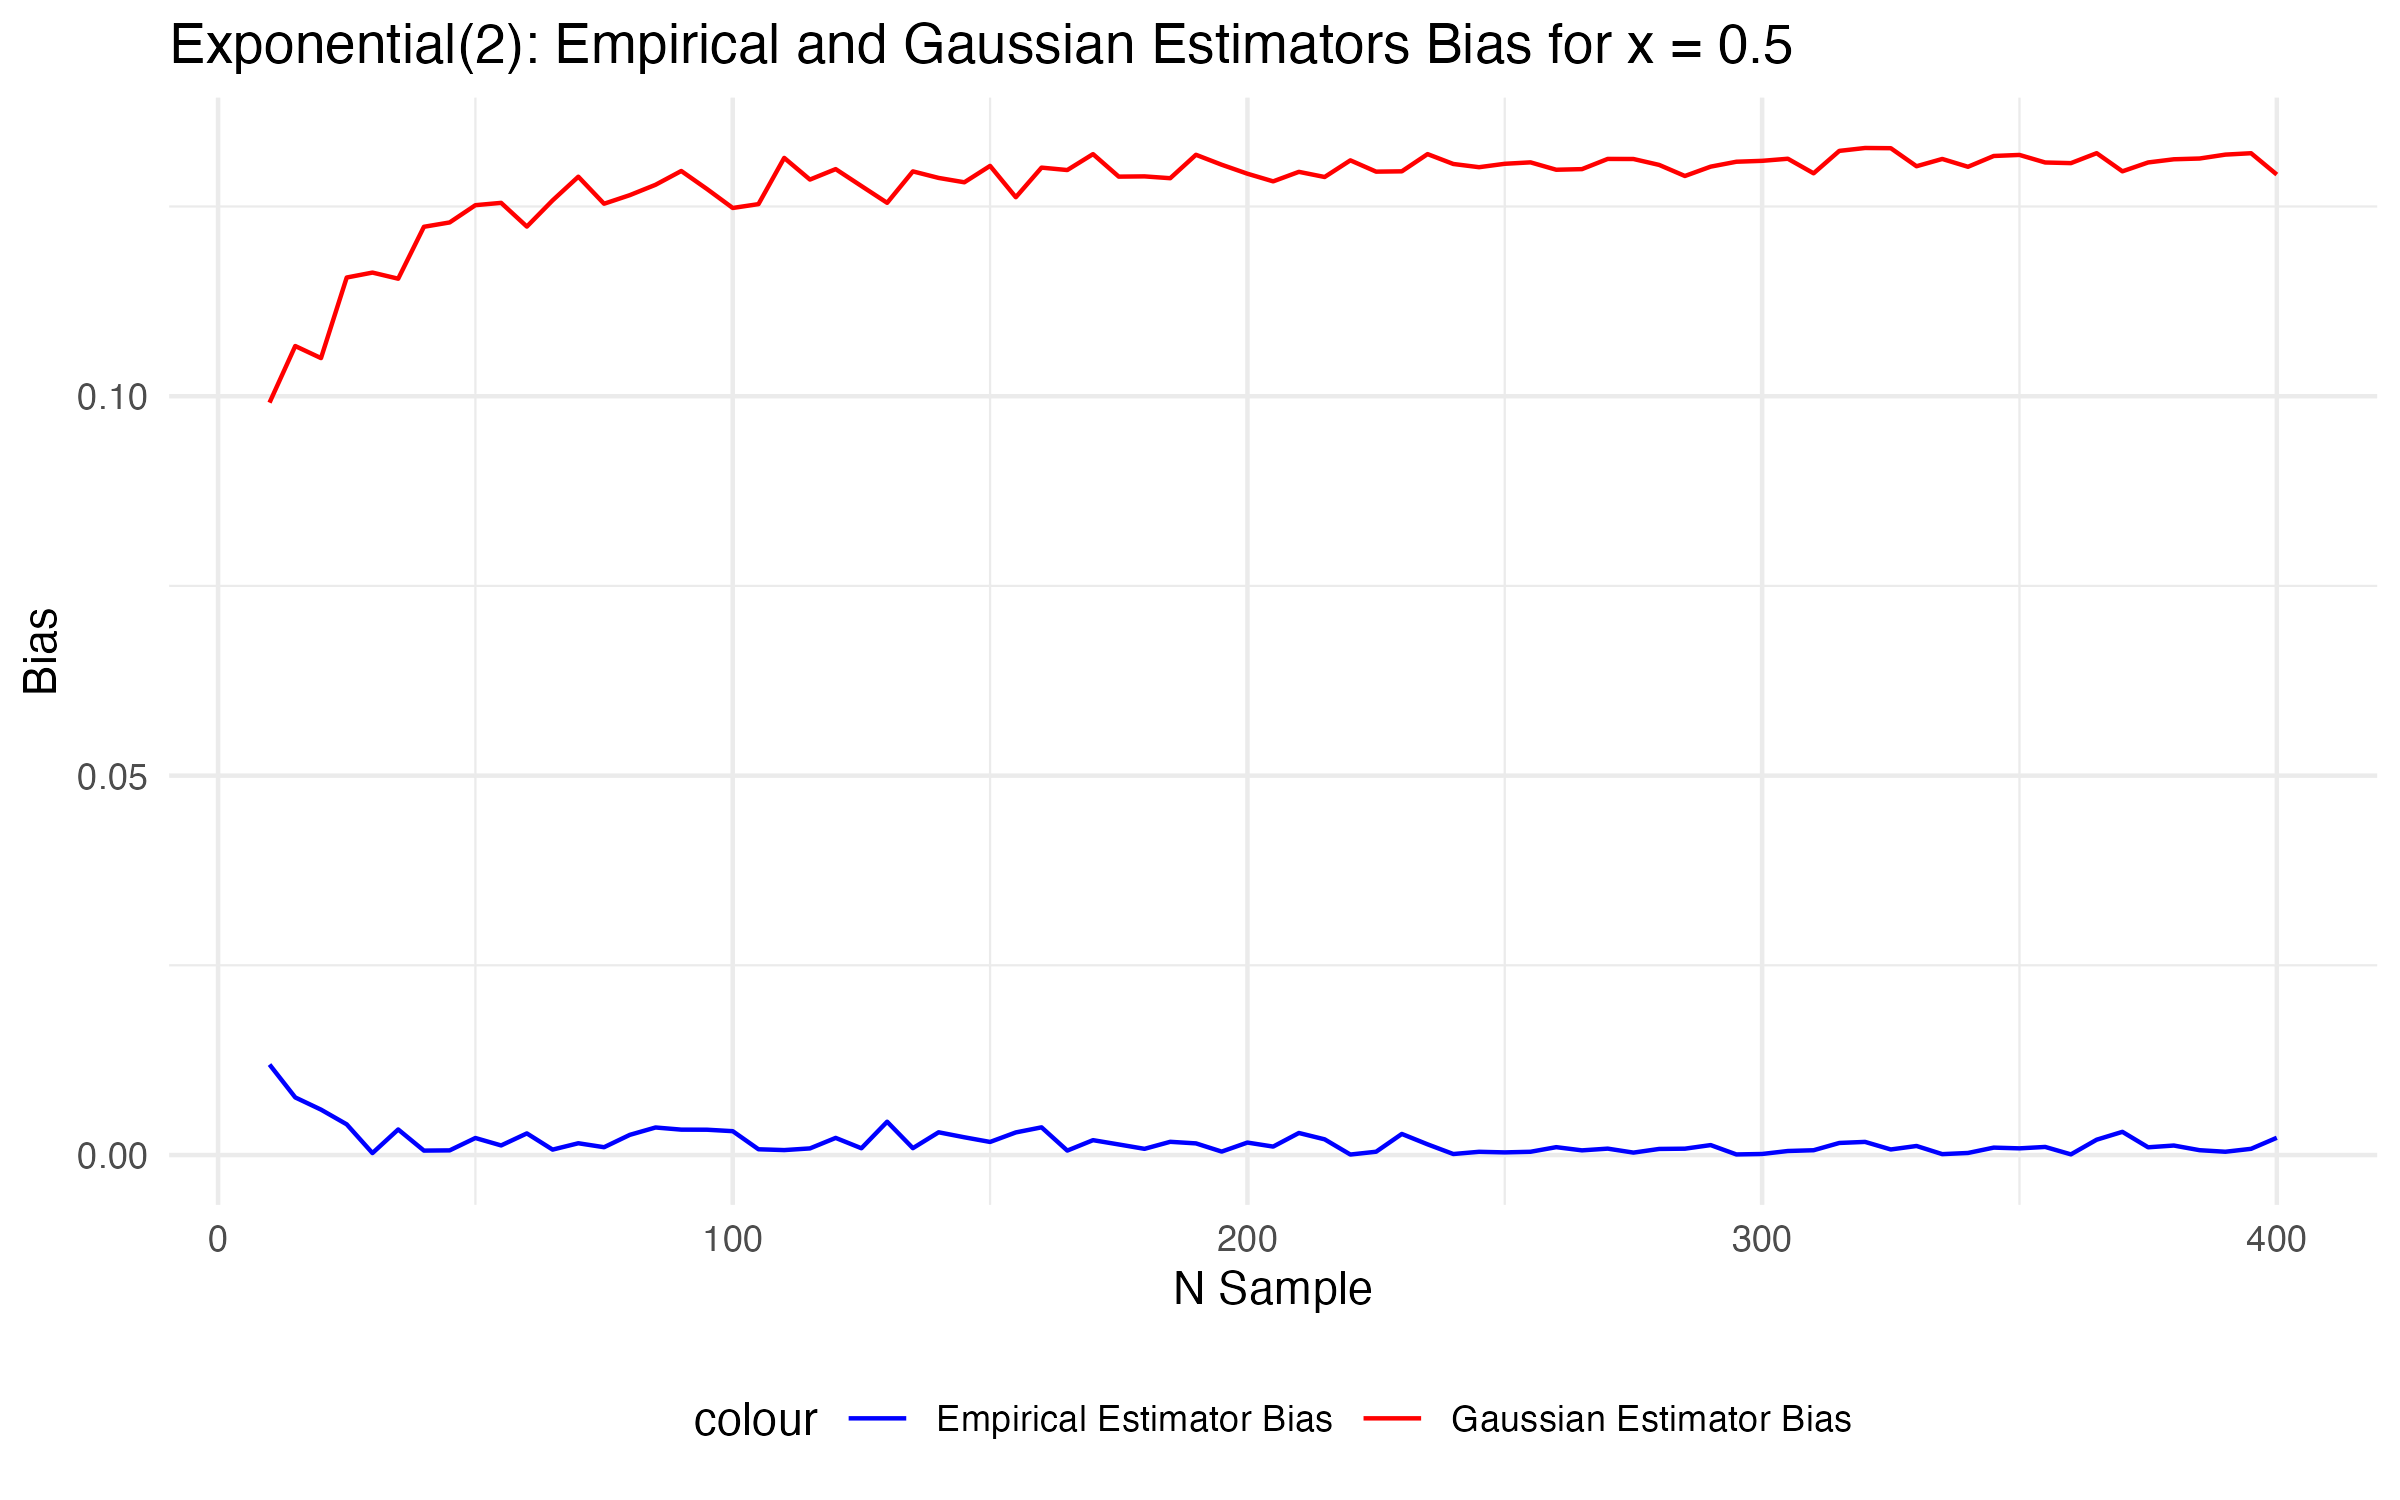
\includegraphics[width=115px]{q2d-plots/bias_x5_exponential.png}
  \includegraphics[width=115px]{q2d-plots/bias_x5_log_normal_1_1.png}
  \includegraphics[width=115px]{q2d-plots/bias_x5_log_normal_1_2.png}
  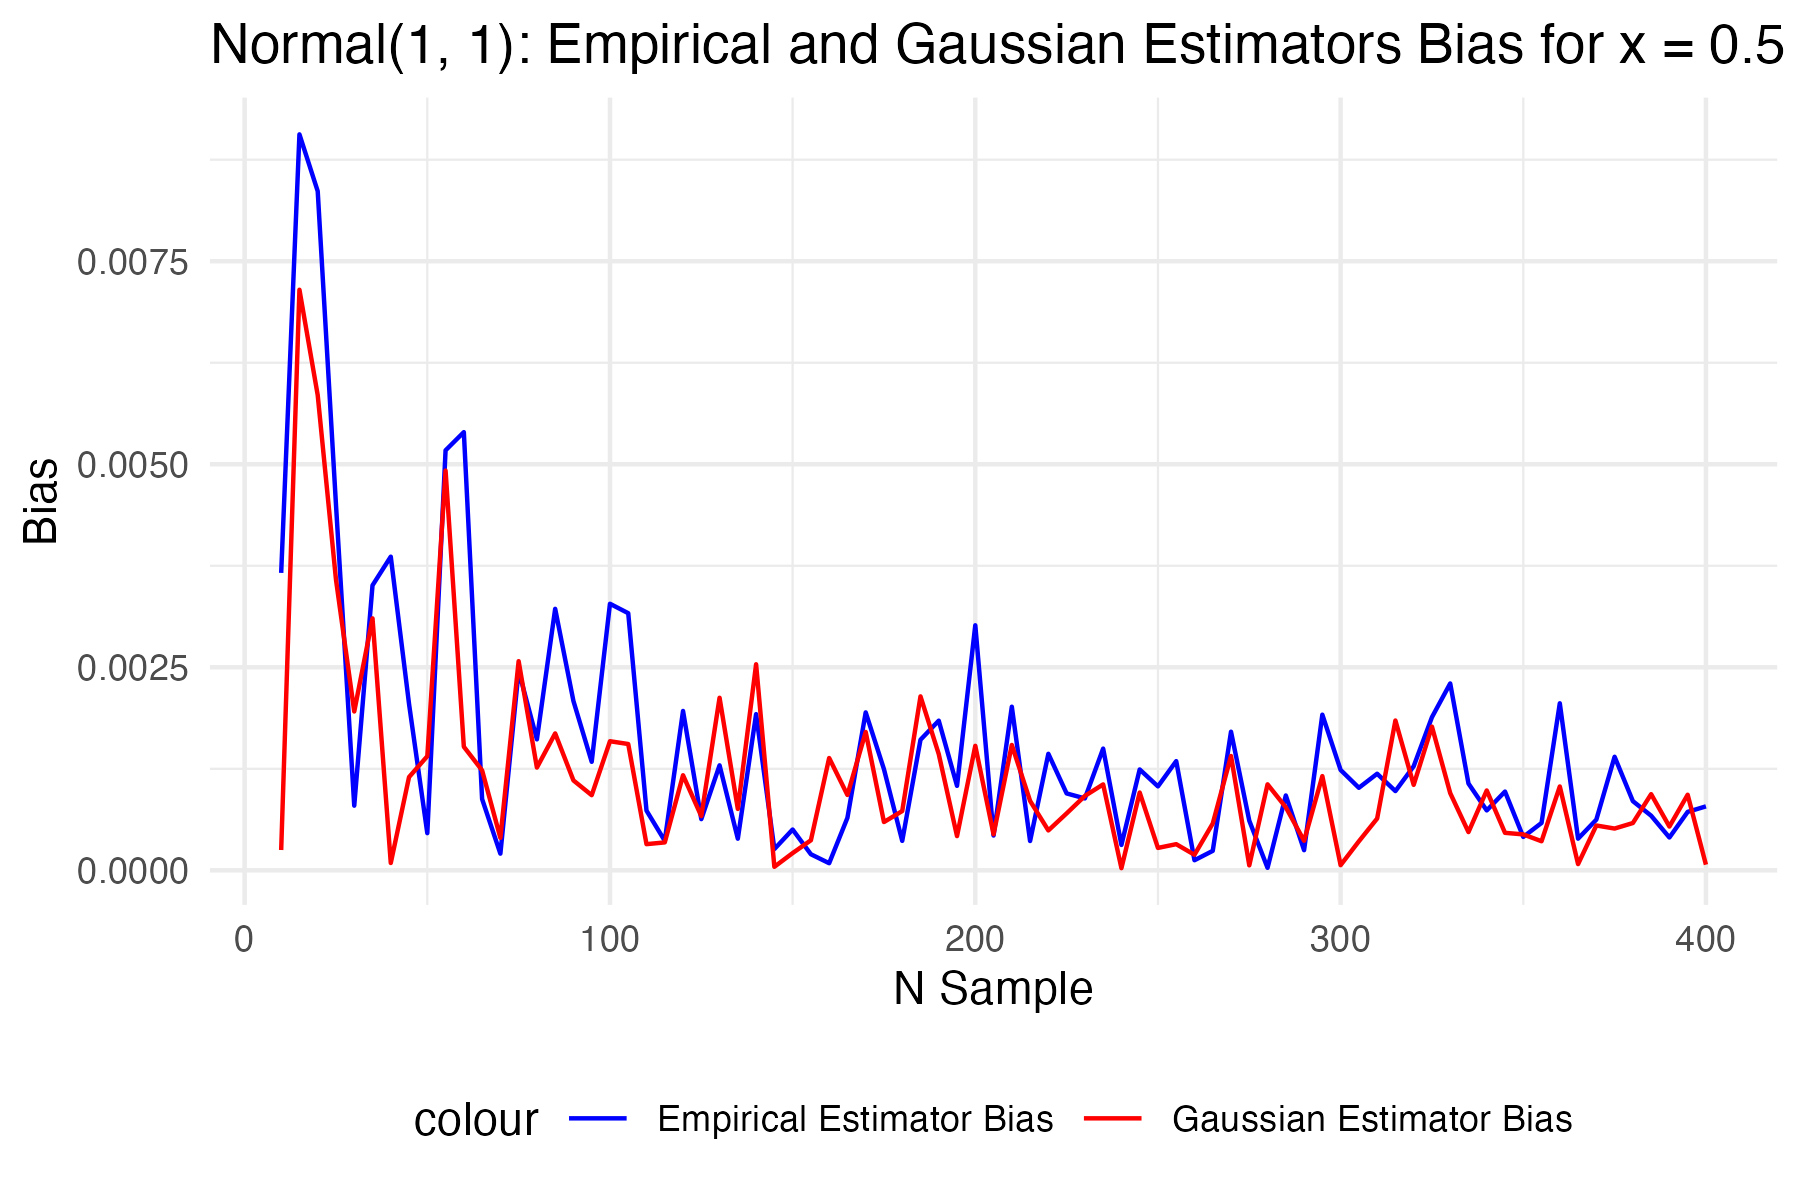
\includegraphics[width=115px]{q2d-plots/bias_x5_normal.png}
  \includegraphics[width=115px]{q2d-plots/bias_x5_t_student_10.png}
  \includegraphics[width=115px]{q2d-plots/bias_x5_t_student_70.png}
  \includegraphics[width=115px]{q2d-plots/bias_x5_t_student_150.png}
  \label{fig:bias_x5}
\end{figure}

\subsubsection*{Variance for $x = 0.5$}

\begin{figure}[H]
  \centering
  \includegraphics[width=115px]{q2d-plots/variance_x5_gamma_1_1.png}
  \includegraphics[width=115px]{q2d-plots/variance_x5_gamma_3_2.png}
  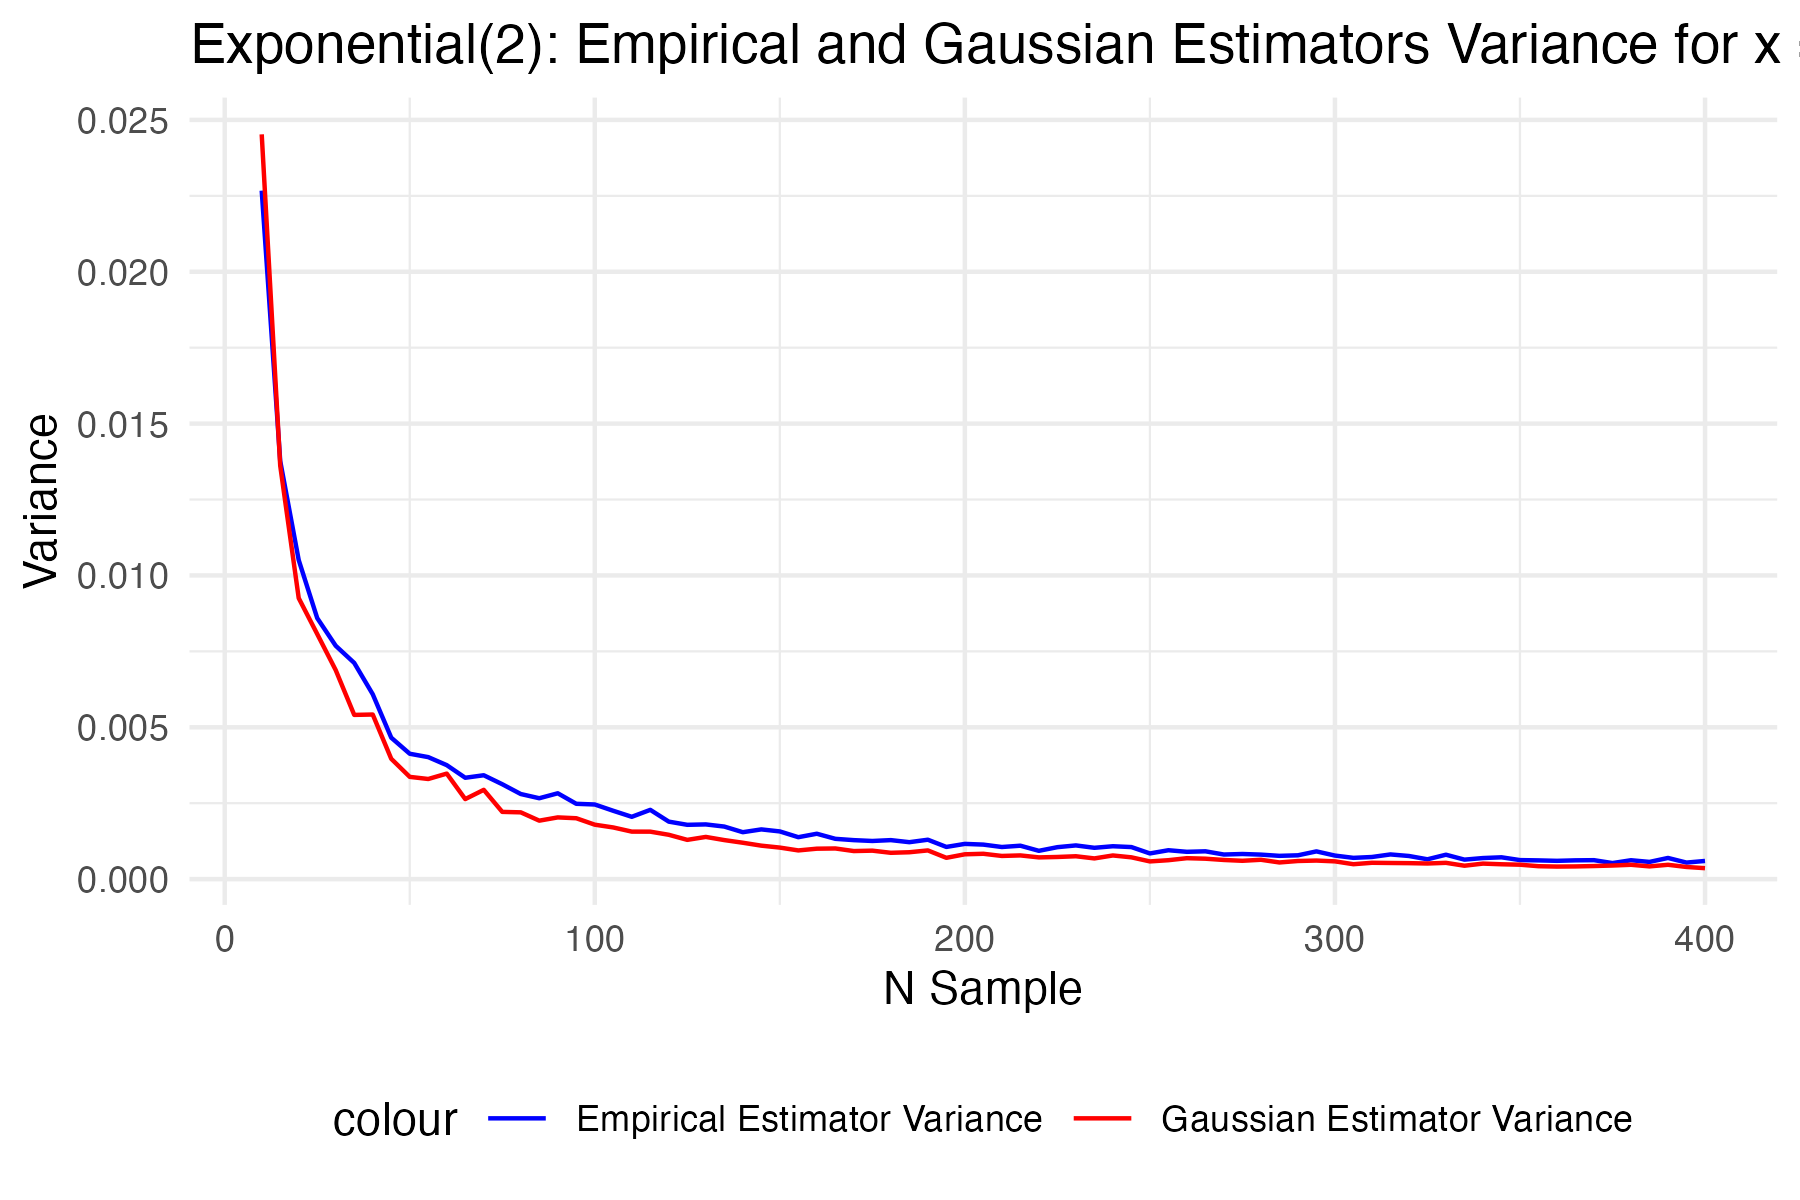
\includegraphics[width=115px]{q2d-plots/variance_x5_exponential.png}
  \includegraphics[width=115px]{q2d-plots/variance_x5_log_normal_1_1.png}
  \includegraphics[width=115px]{q2d-plots/variance_x5_log_normal_1_2.png}
  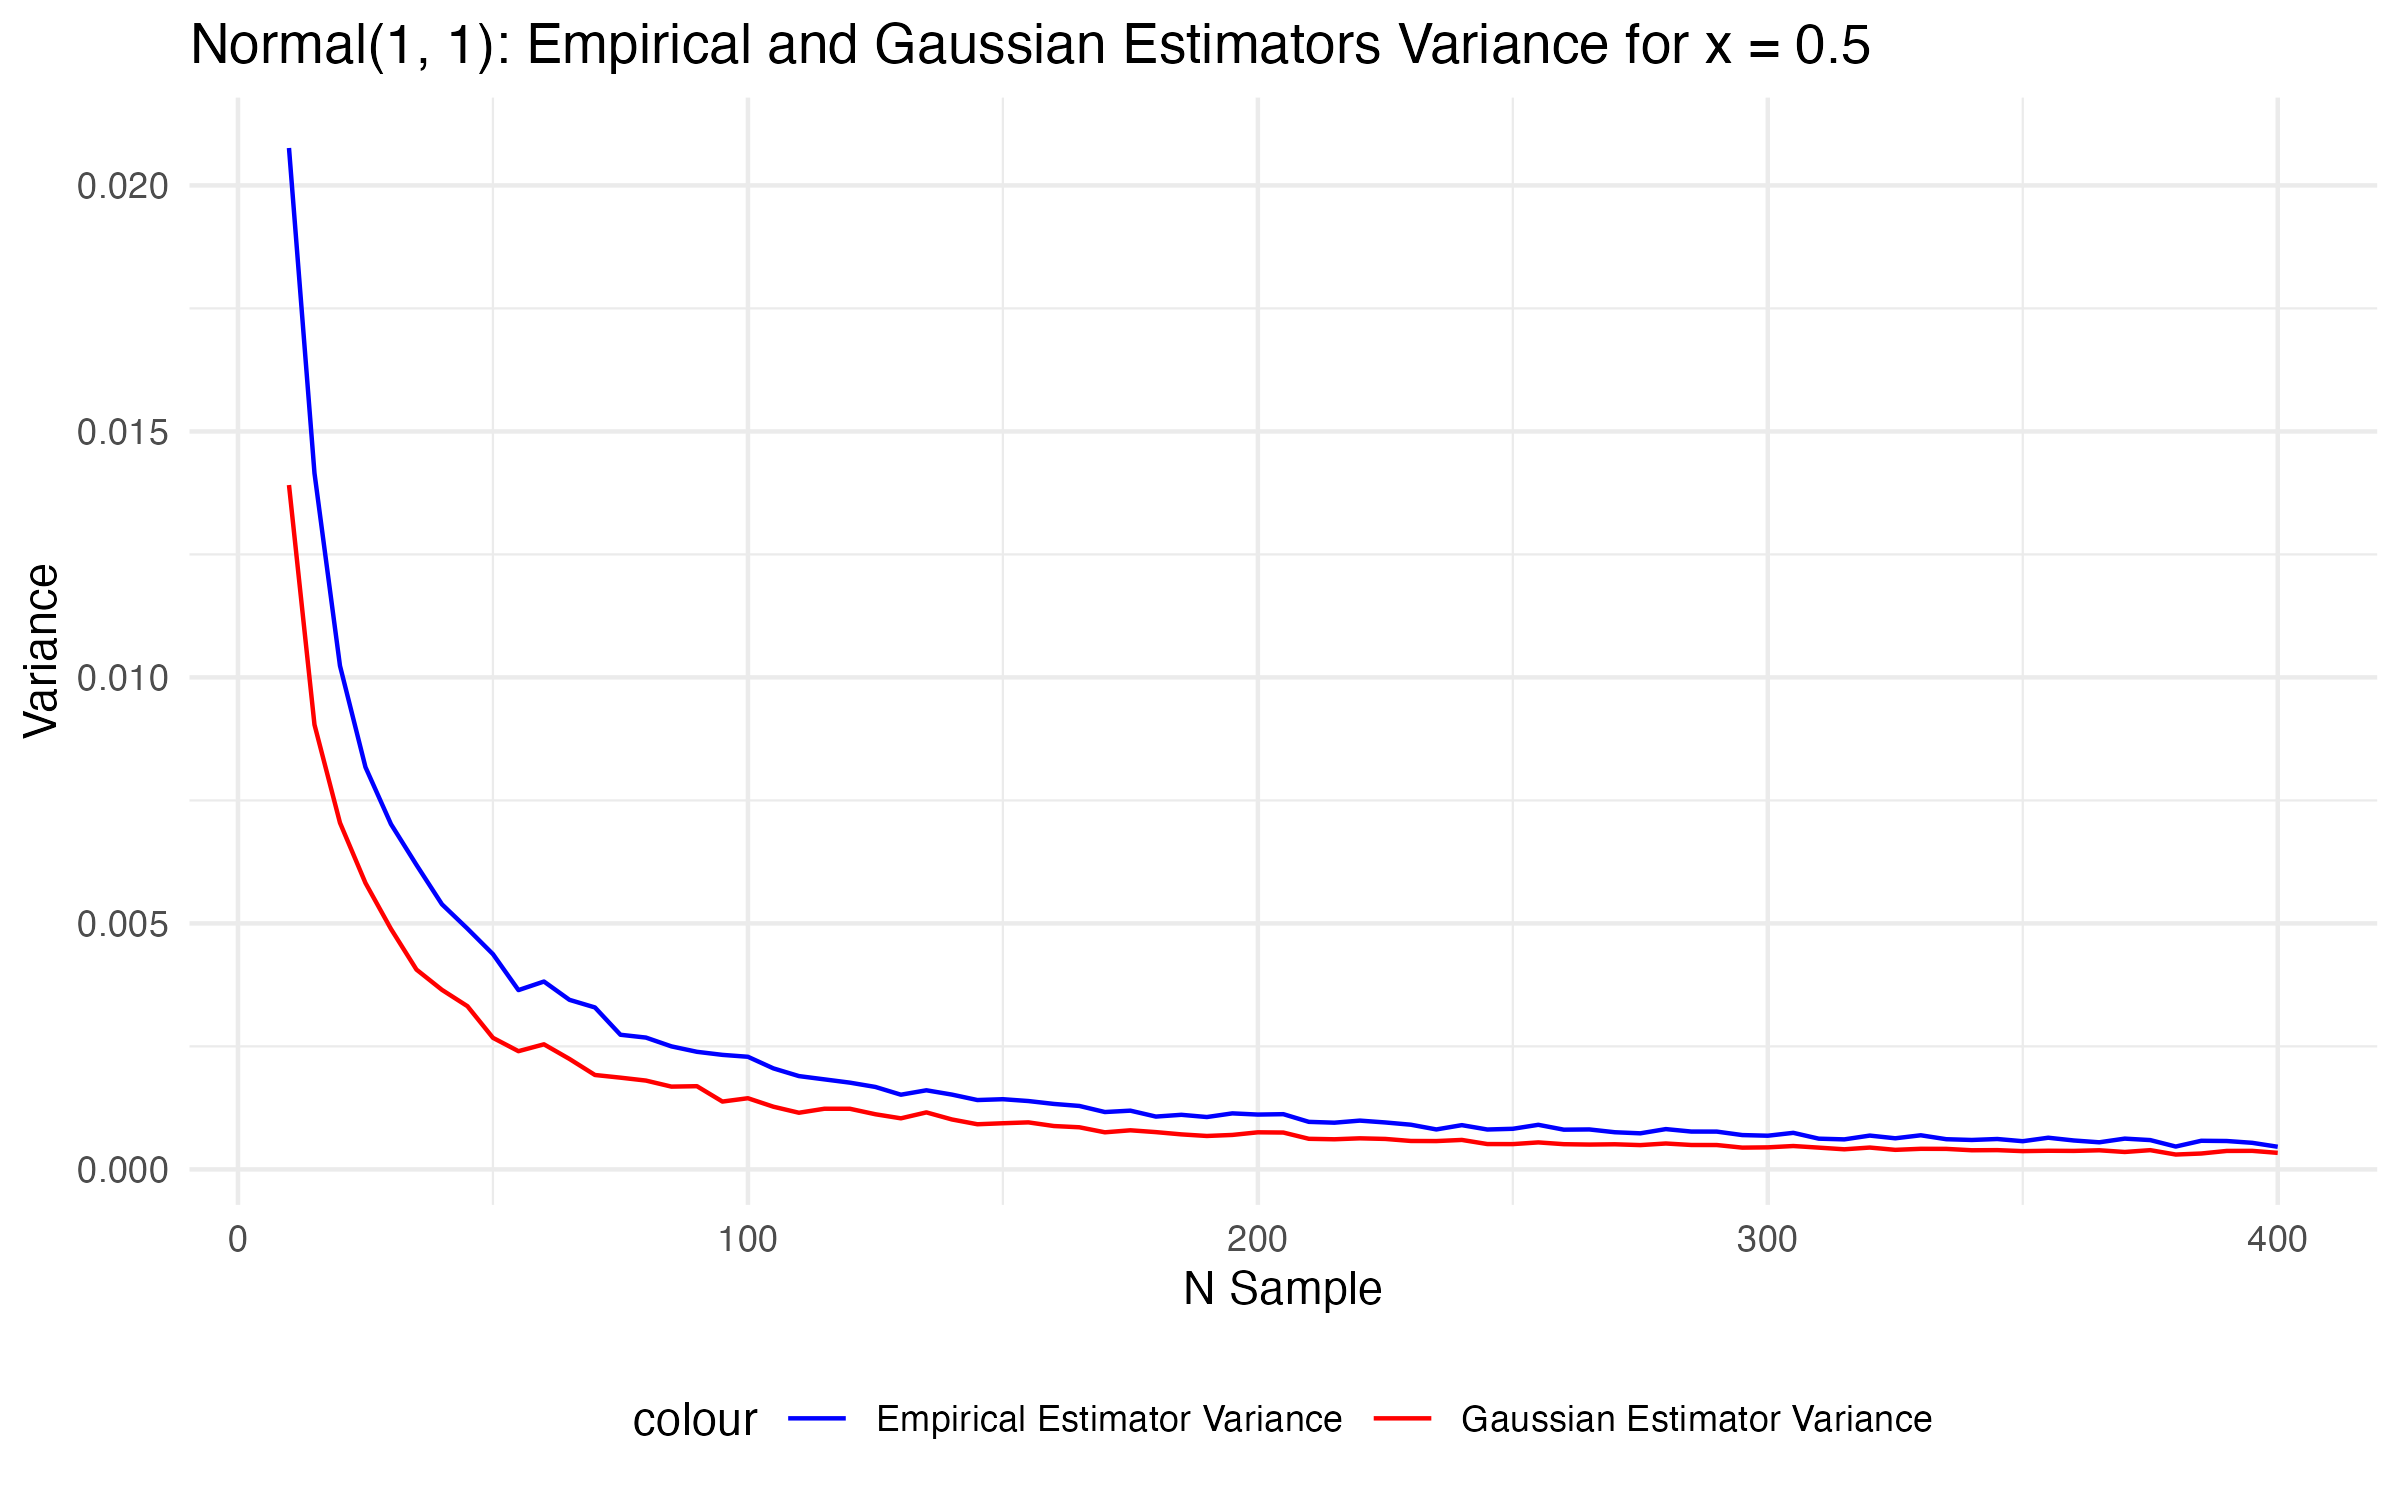
\includegraphics[width=115px]{q2d-plots/variance_x5_normal.png}
  \includegraphics[width=115px]{q2d-plots/variance_x5_t_student_10.png}
  \includegraphics[width=115px]{q2d-plots/variance_x5_t_student_70.png}
  \includegraphics[width=115px]{q2d-plots/variance_x5_t_student_150.png}
  \label{fig:variance_x5}
\end{figure}

\subsubsection*{MSE for $x = 0.5$}

\begin{figure}[H]
  \centering
  \includegraphics[width=115px]{q2d-plots/mse_x5_gamma_1_1.png}
  \includegraphics[width=115px]{q2d-plots/mse_x5_gamma_3_2.png}
  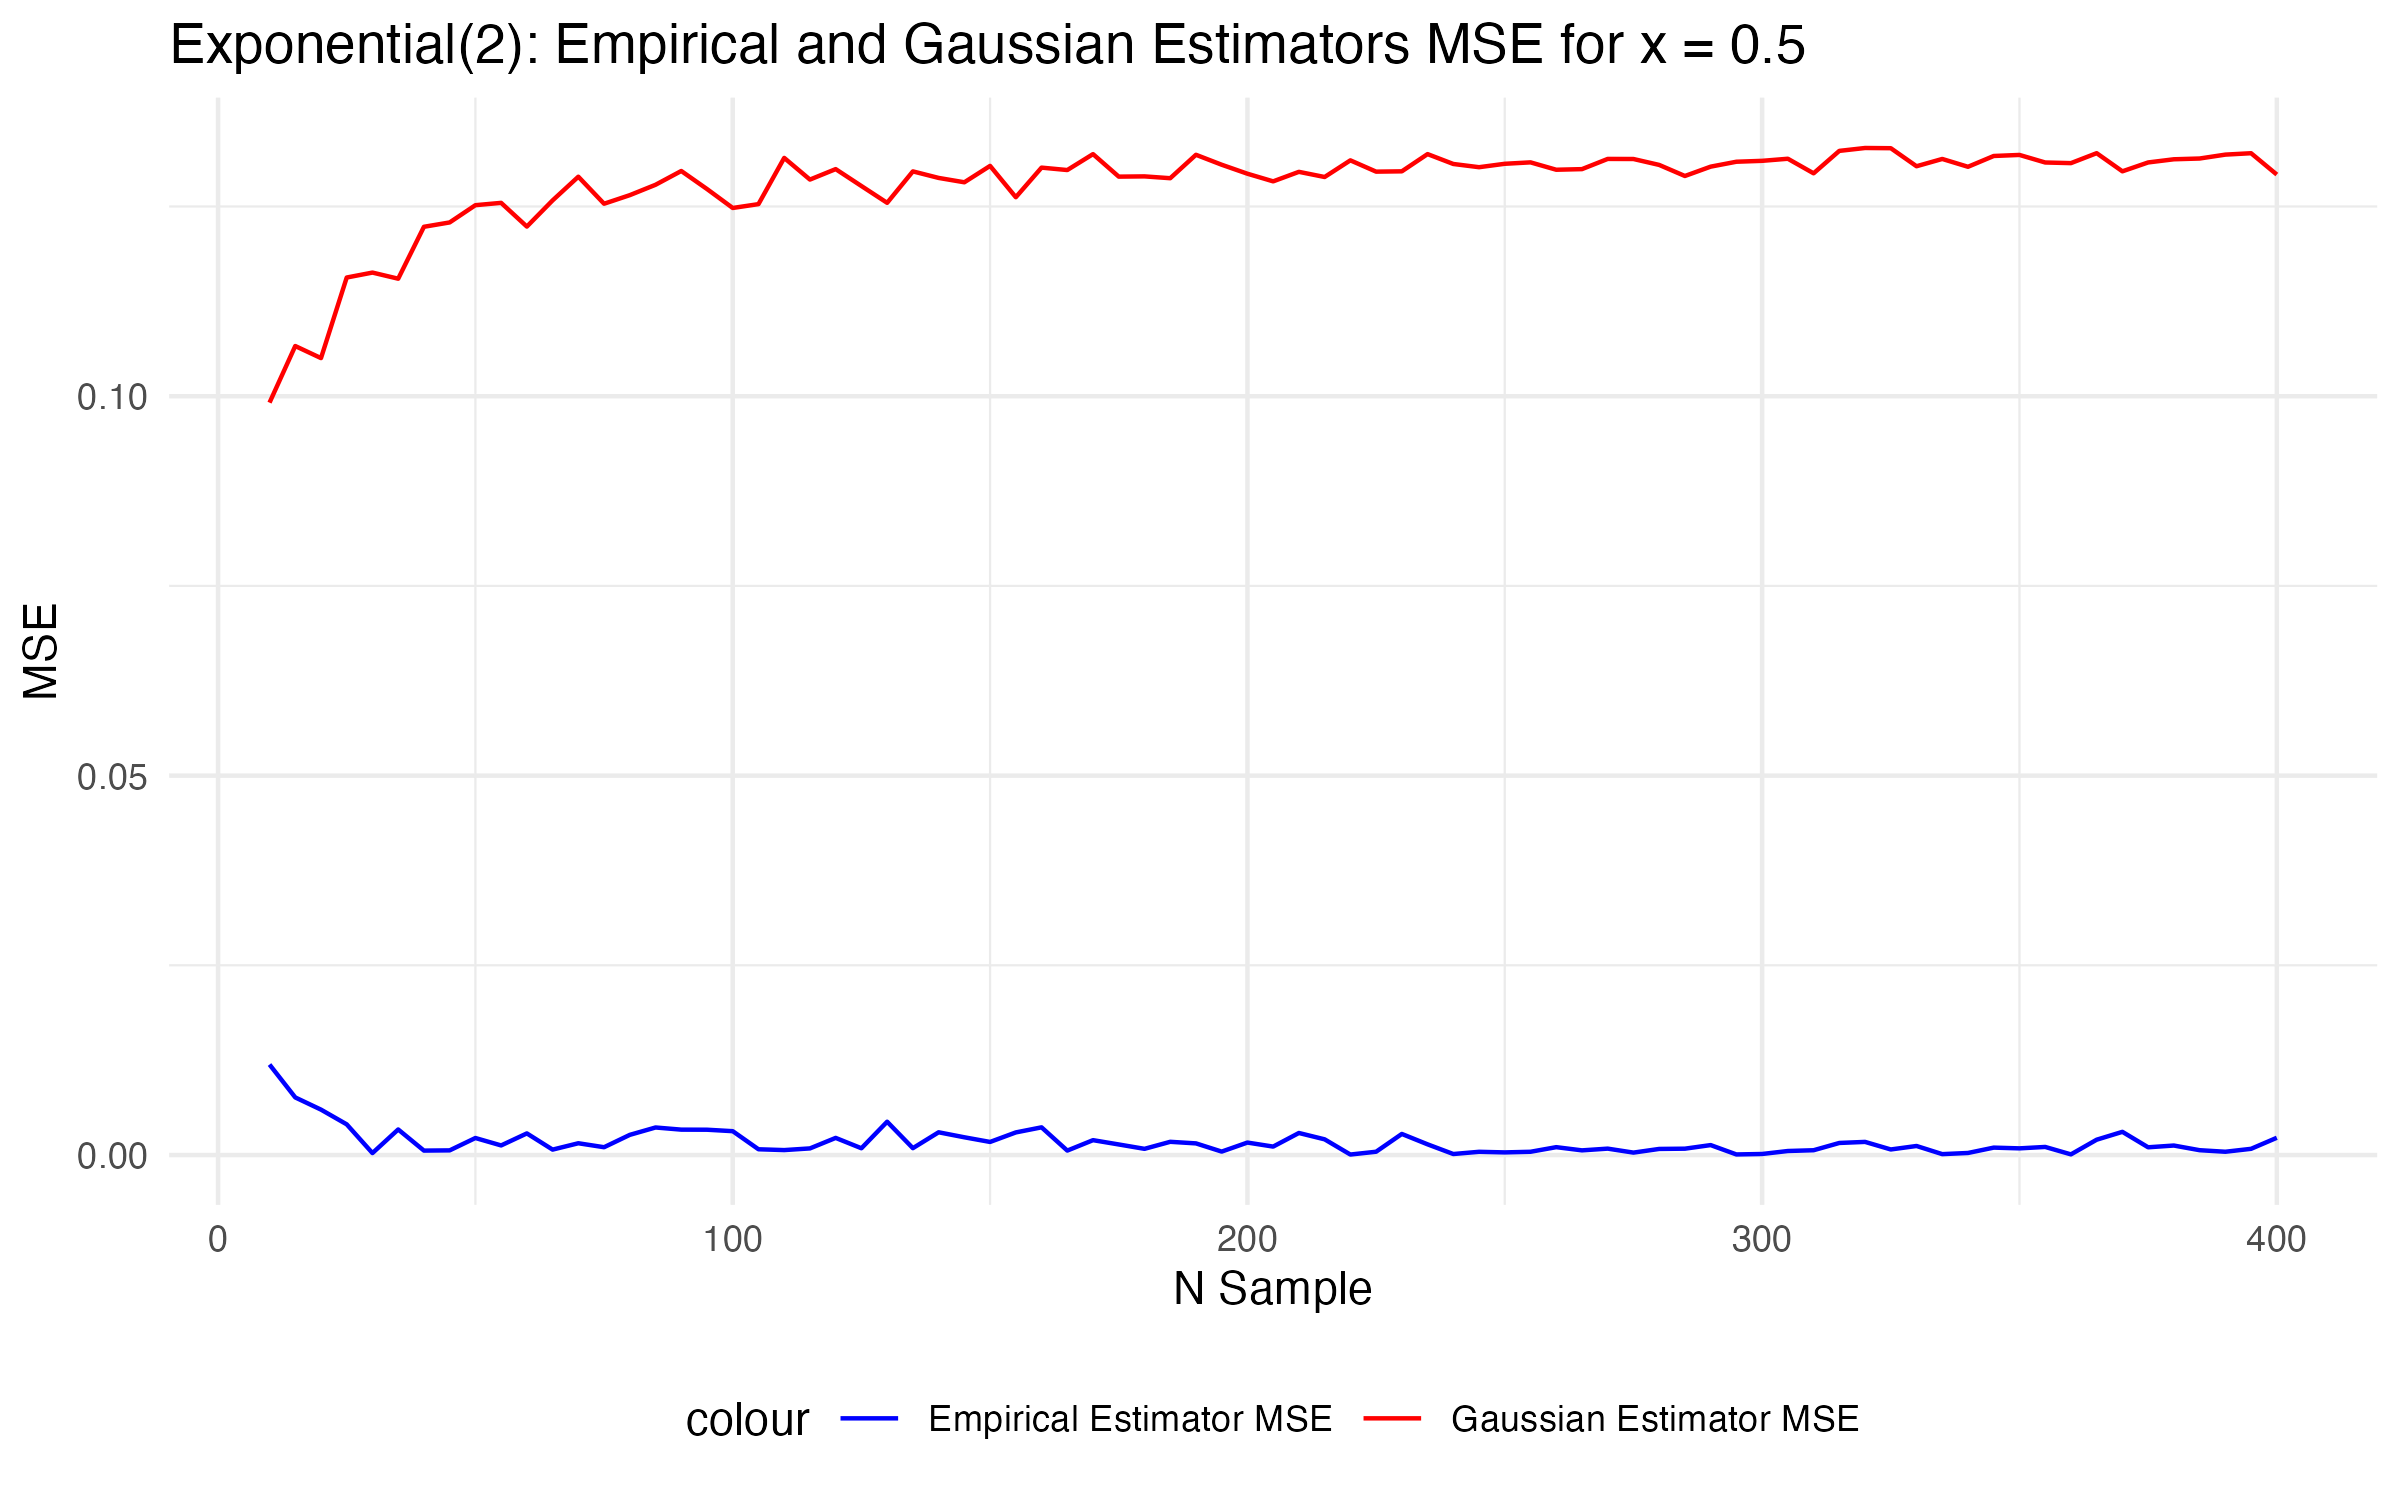
\includegraphics[width=115px]{q2d-plots/mse_x5_exponential.png}
  \includegraphics[width=115px]{q2d-plots/mse_x5_log_normal_1_1.png}
  \includegraphics[width=115px]{q2d-plots/mse_x5_log_normal_1_2.png}
  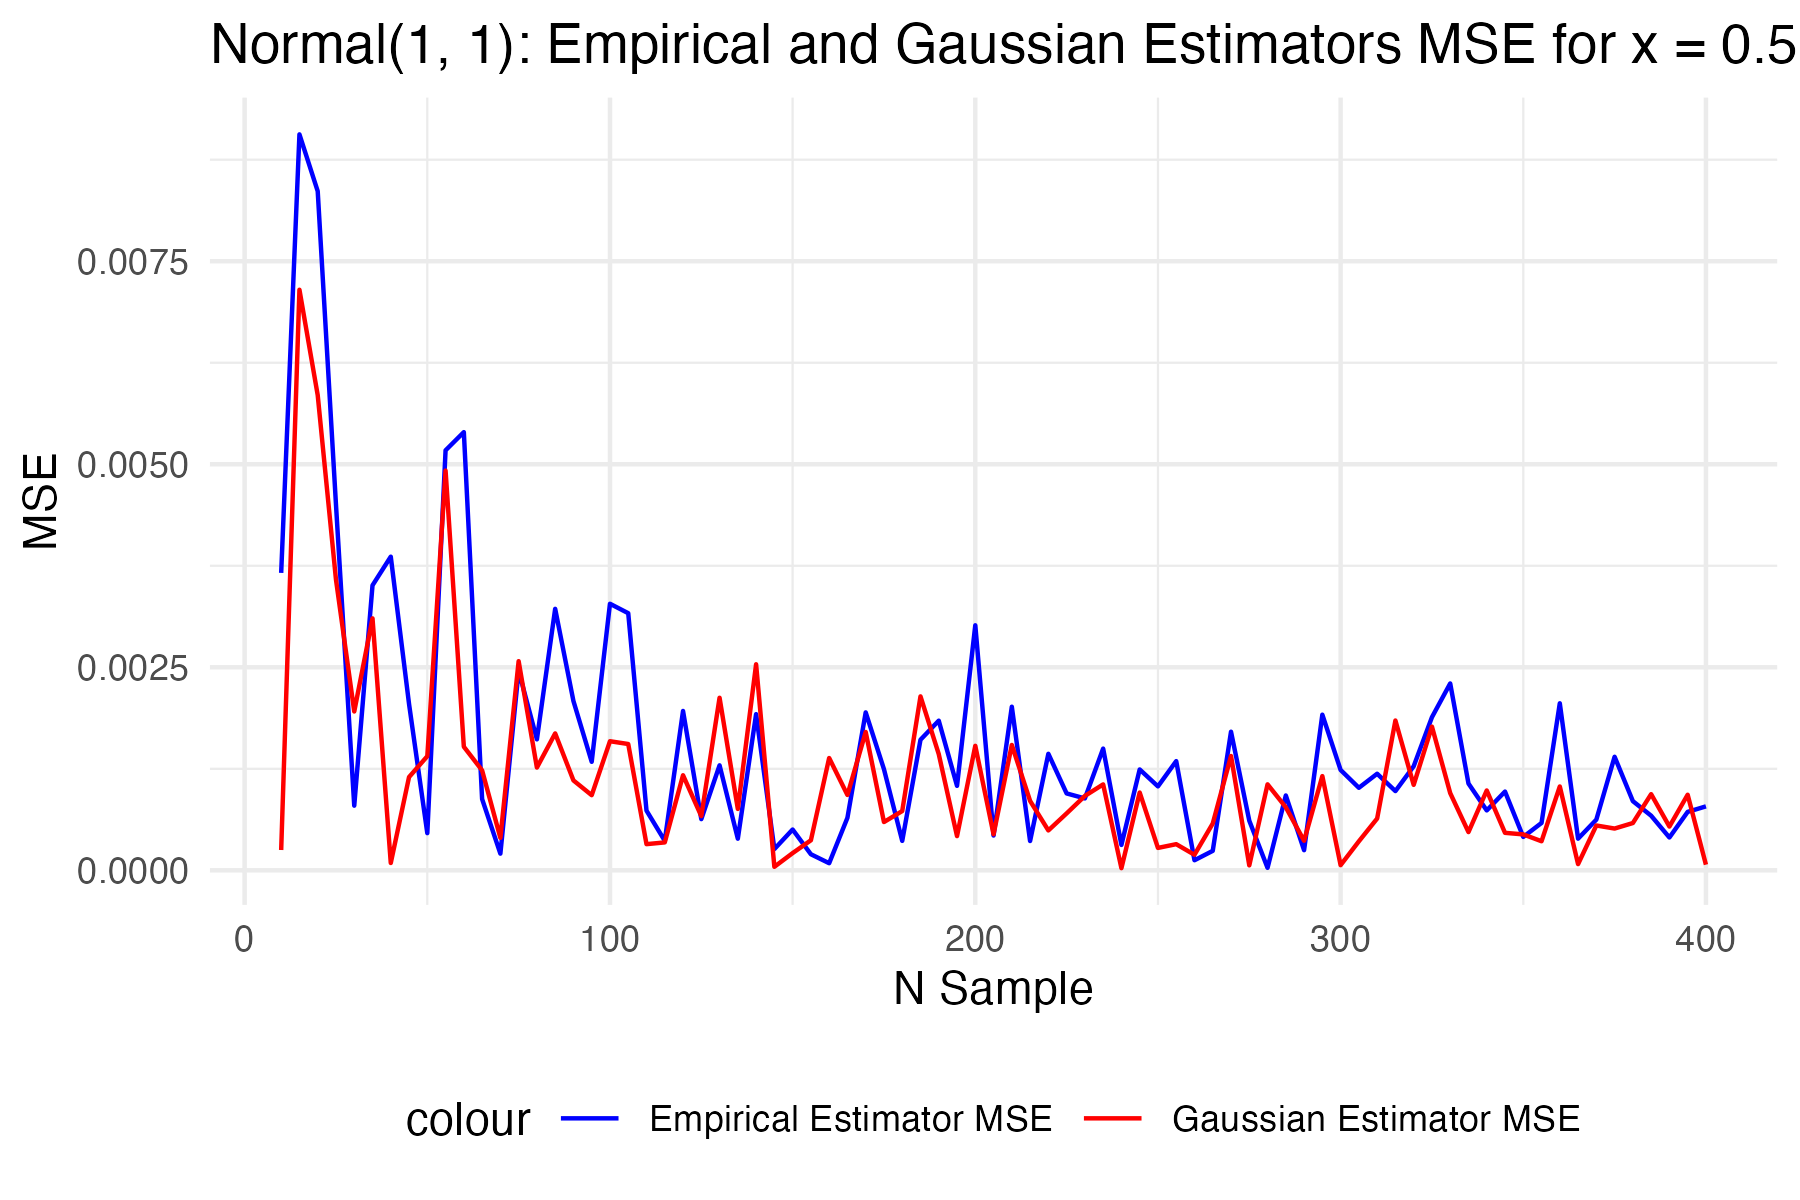
\includegraphics[width=115px]{q2d-plots/mse_x5_normal.png}
  \includegraphics[width=115px]{q2d-plots/mse_x5_t_student_10.png}
  \includegraphics[width=115px]{q2d-plots/mse_x5_t_student_70.png}
  \includegraphics[width=115px]{q2d-plots/mse_x5_t_student_150.png}
  \label{fig:mse_x5}
\end{figure}

\subsubsection*{CI for $x = 0.5$}

\begin{figure}[H]
  \centering
  \includegraphics[width=115px]{q2d-plots/ci_x5_gamma_1_1.png}
  \includegraphics[width=115px]{q2d-plots/ci_x5_gamma_3_2.png}
  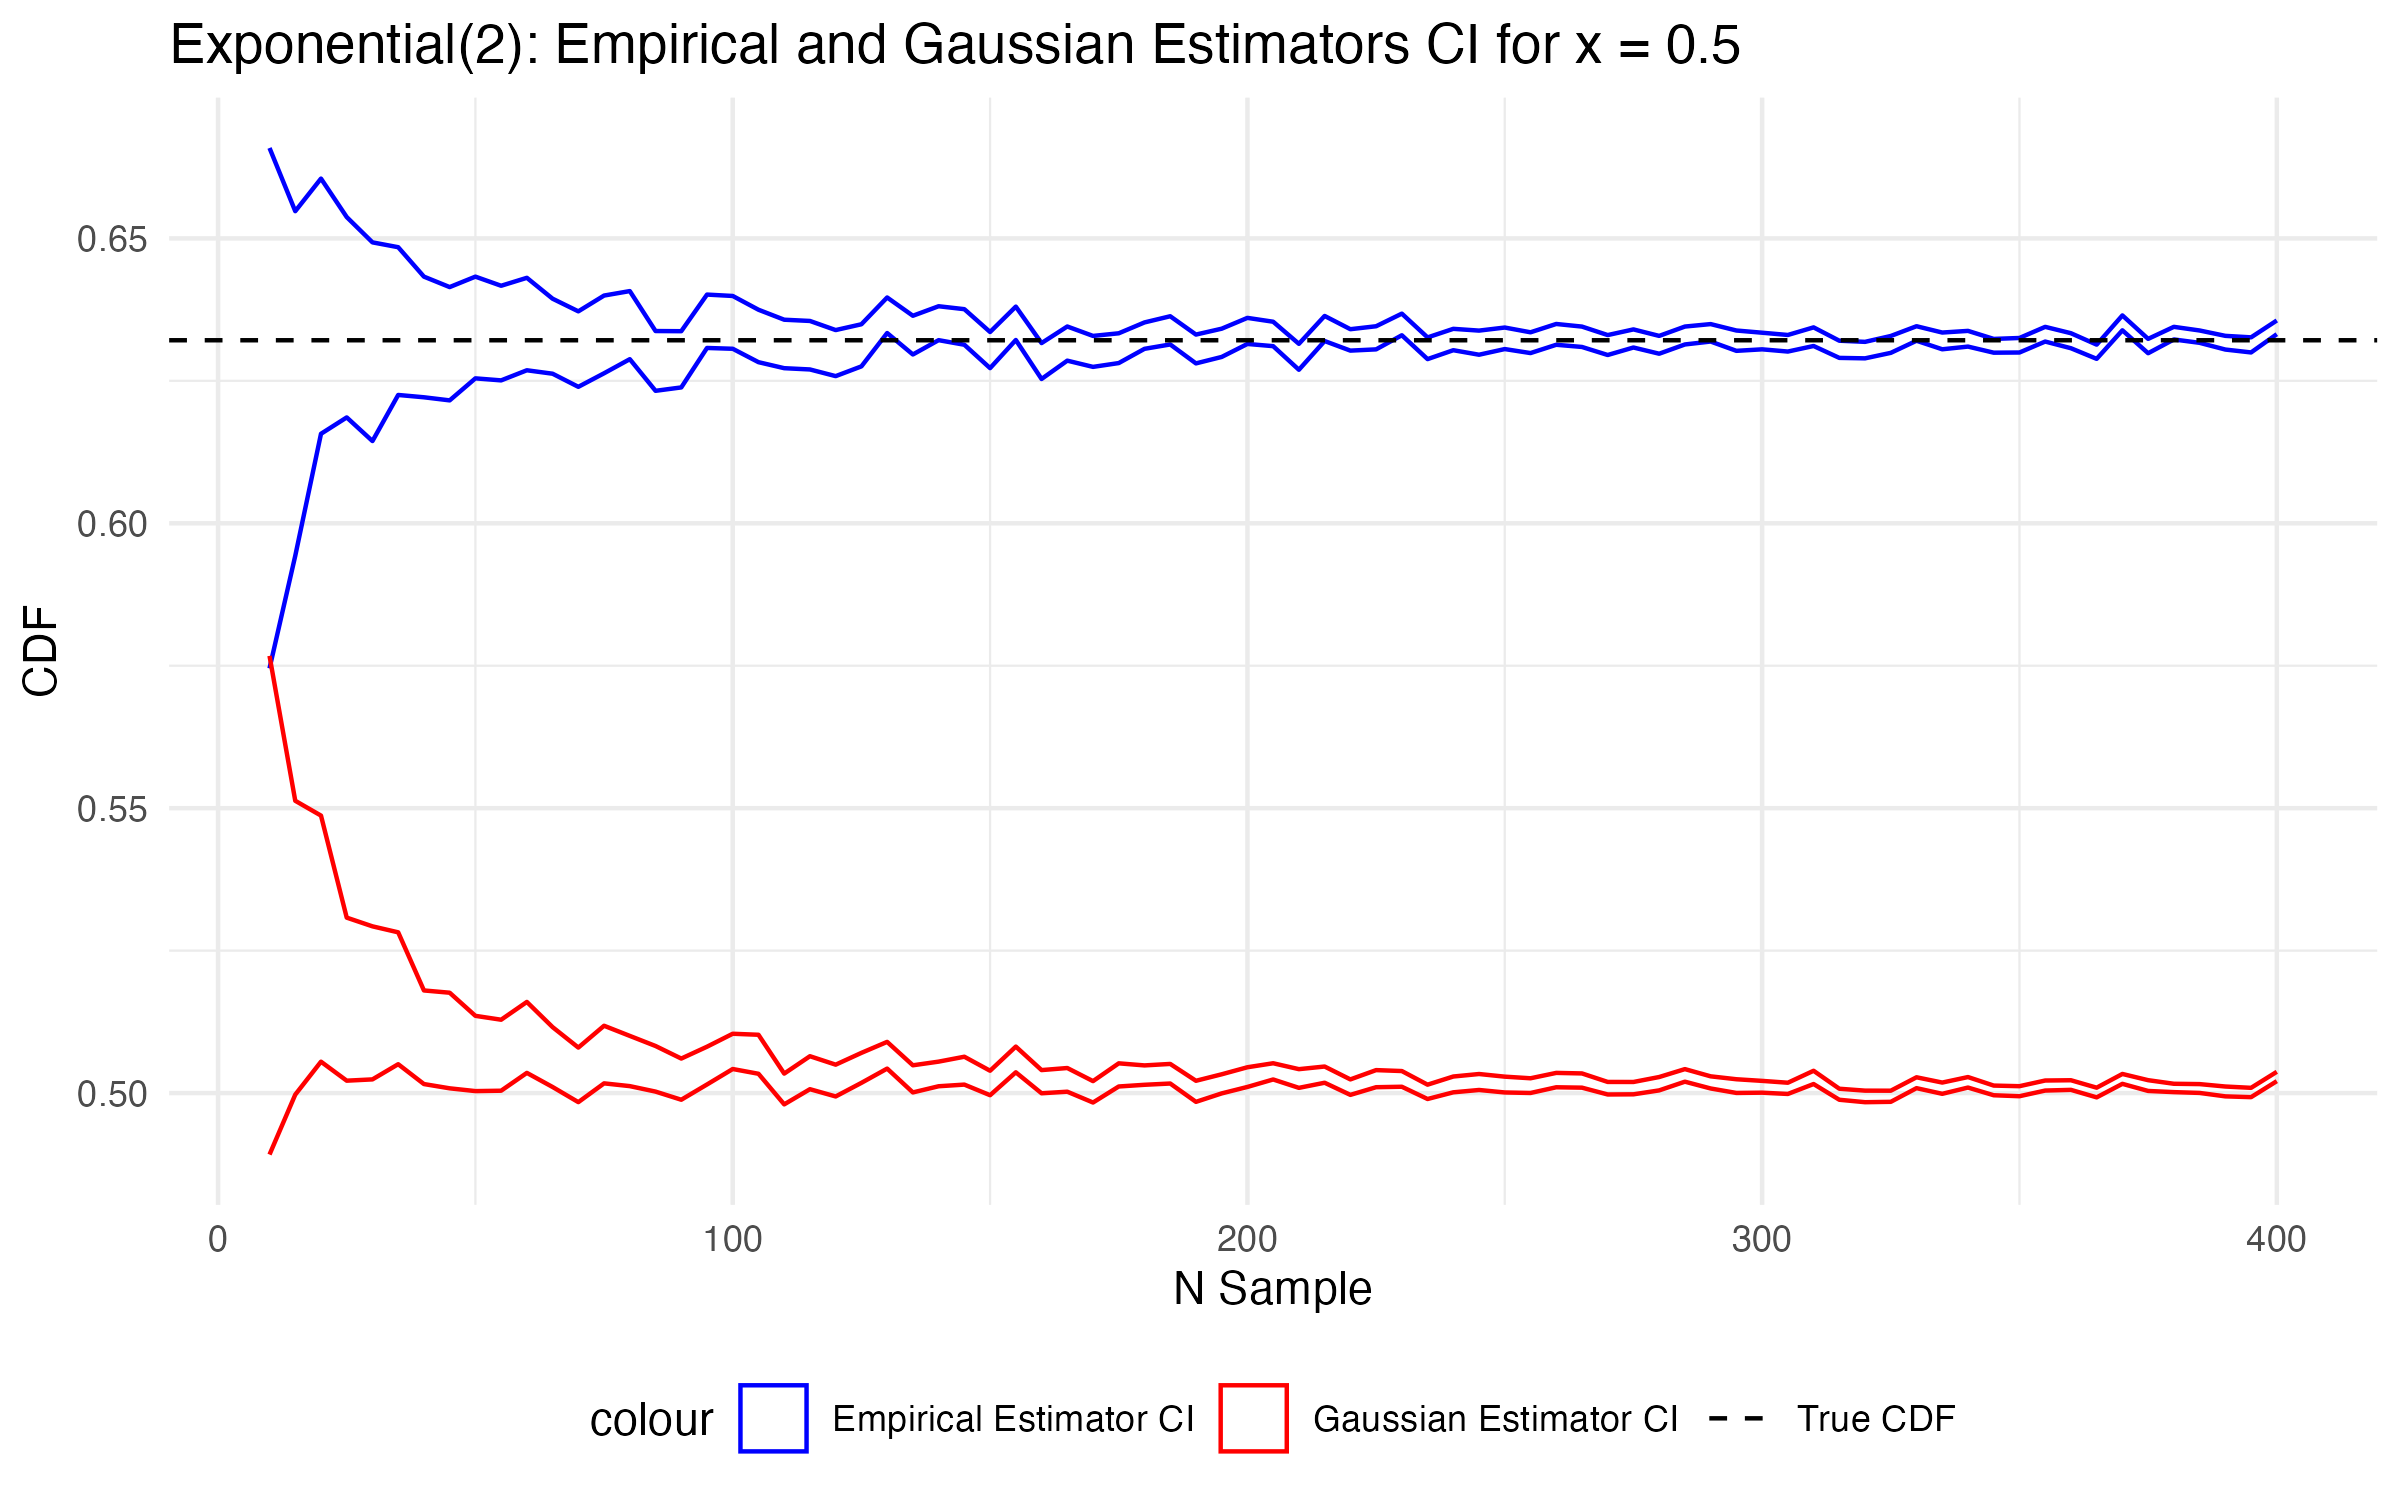
\includegraphics[width=115px]{q2d-plots/ci_x5_exponential.png}
  \includegraphics[width=115px]{q2d-plots/ci_x5_log_normal_1_1.png}
  \includegraphics[width=115px]{q2d-plots/ci_x5_log_normal_1_2.png}
  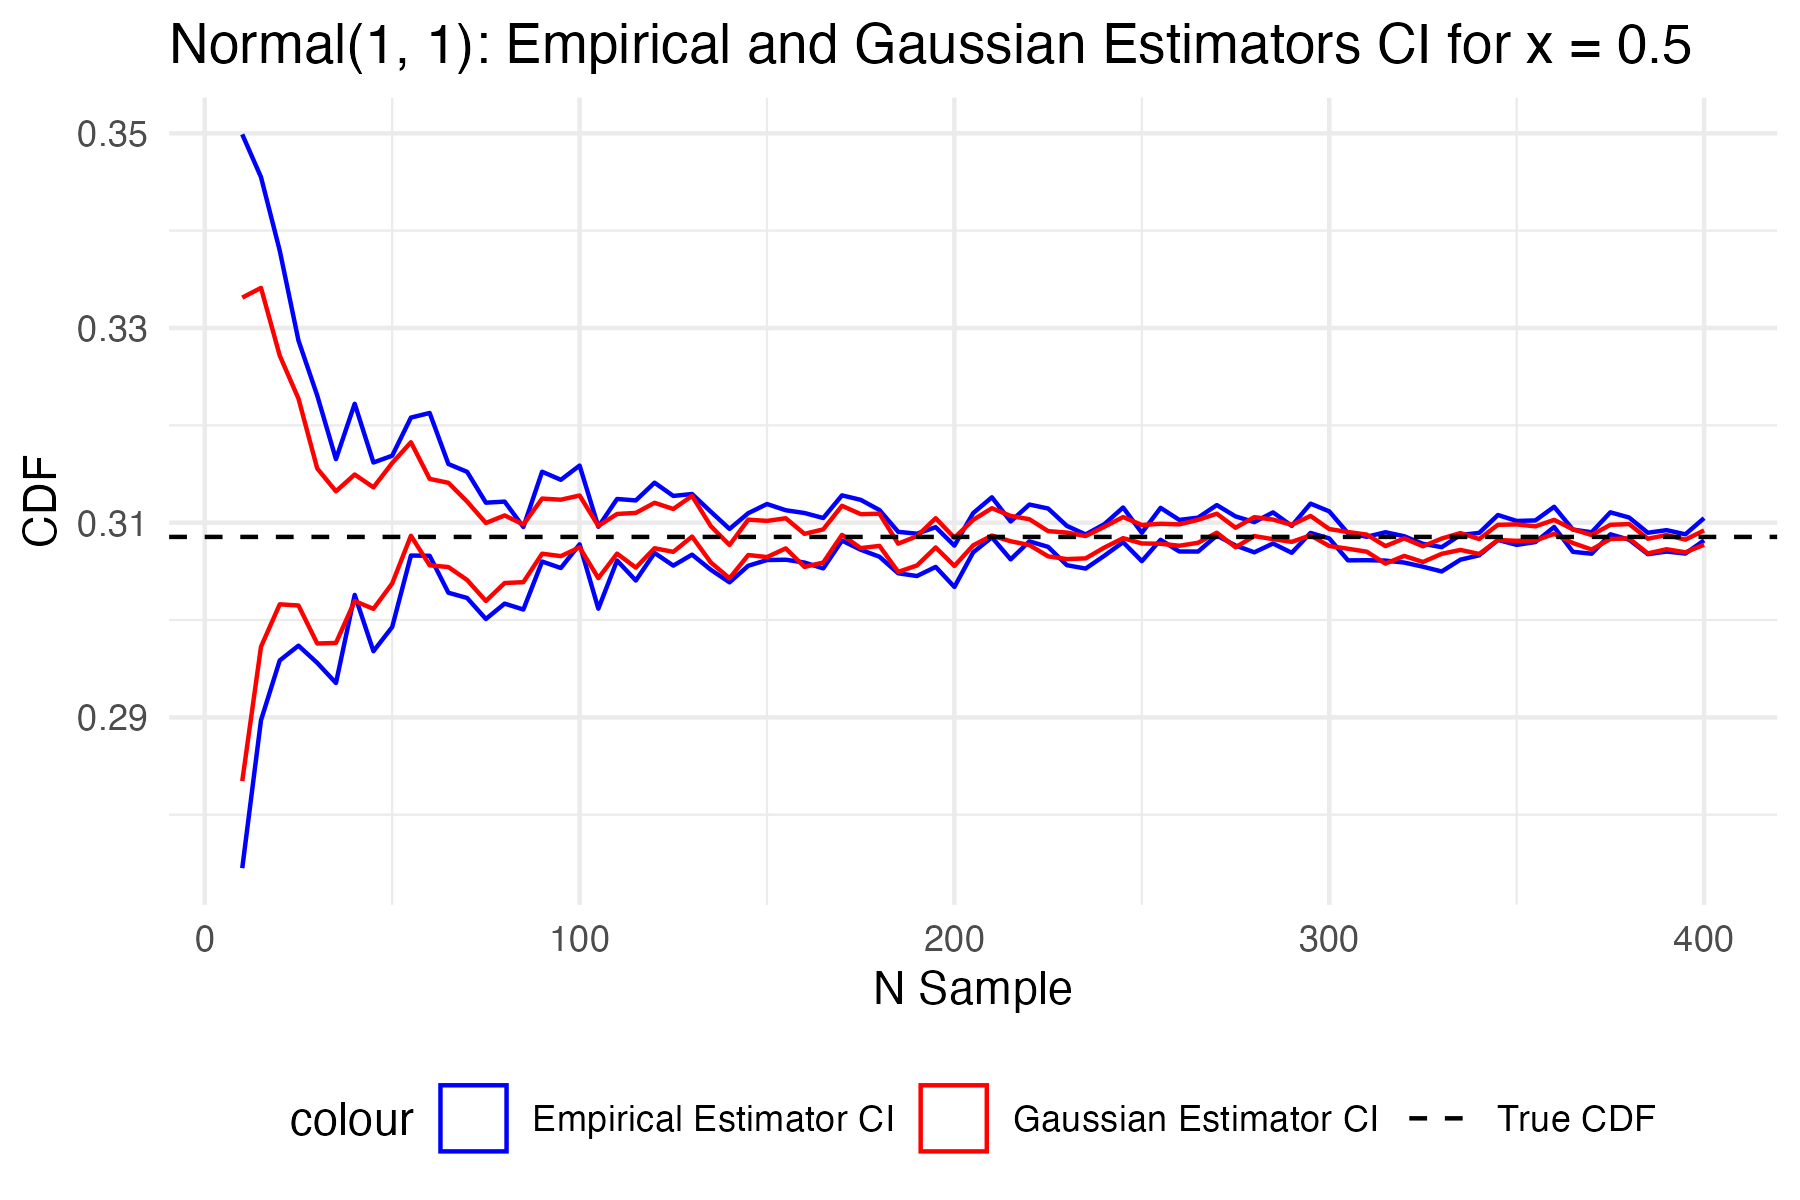
\includegraphics[width=115px]{q2d-plots/ci_x5_normal.png}
  \includegraphics[width=115px]{q2d-plots/ci_x5_t_student_10.png}
  \includegraphics[width=115px]{q2d-plots/ci_x5_t_student_70.png}
  \includegraphics[width=115px]{q2d-plots/ci_x5_t_student_150.png}
  \label{fig:ci_x5}
\end{figure}

\subsubsection*{Bias for $x = 1.5$}

\begin{figure}[H]
  \centering
  \includegraphics[width=115px]{q2d-plots/bias_x15_gamma_1_1.png}
  \includegraphics[width=115px]{q2d-plots/bias_x15_gamma_3_2.png}
  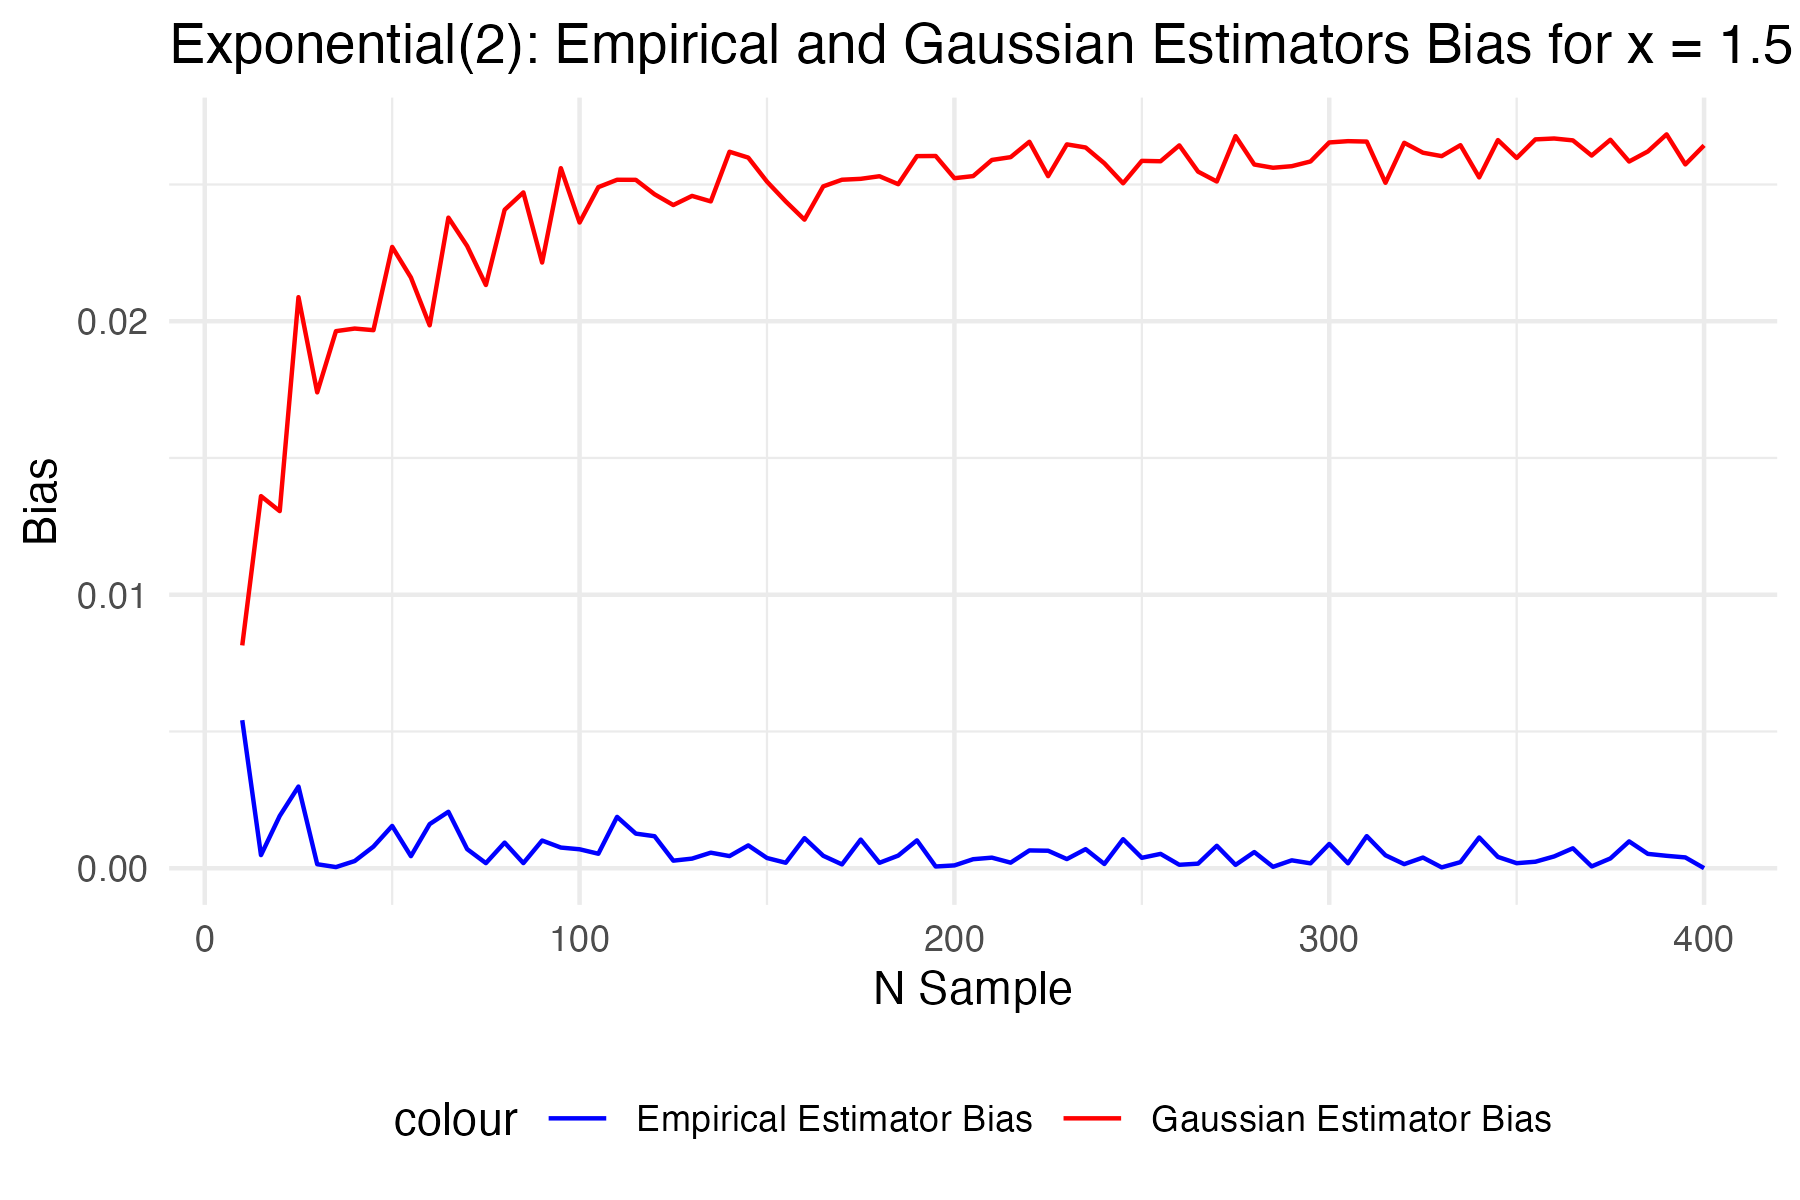
\includegraphics[width=115px]{q2d-plots/bias_x15_exponential.png}
  \includegraphics[width=115px]{q2d-plots/bias_x15_log_normal_1_1.png}
  \includegraphics[width=115px]{q2d-plots/bias_x15_log_normal_1_2.png}
  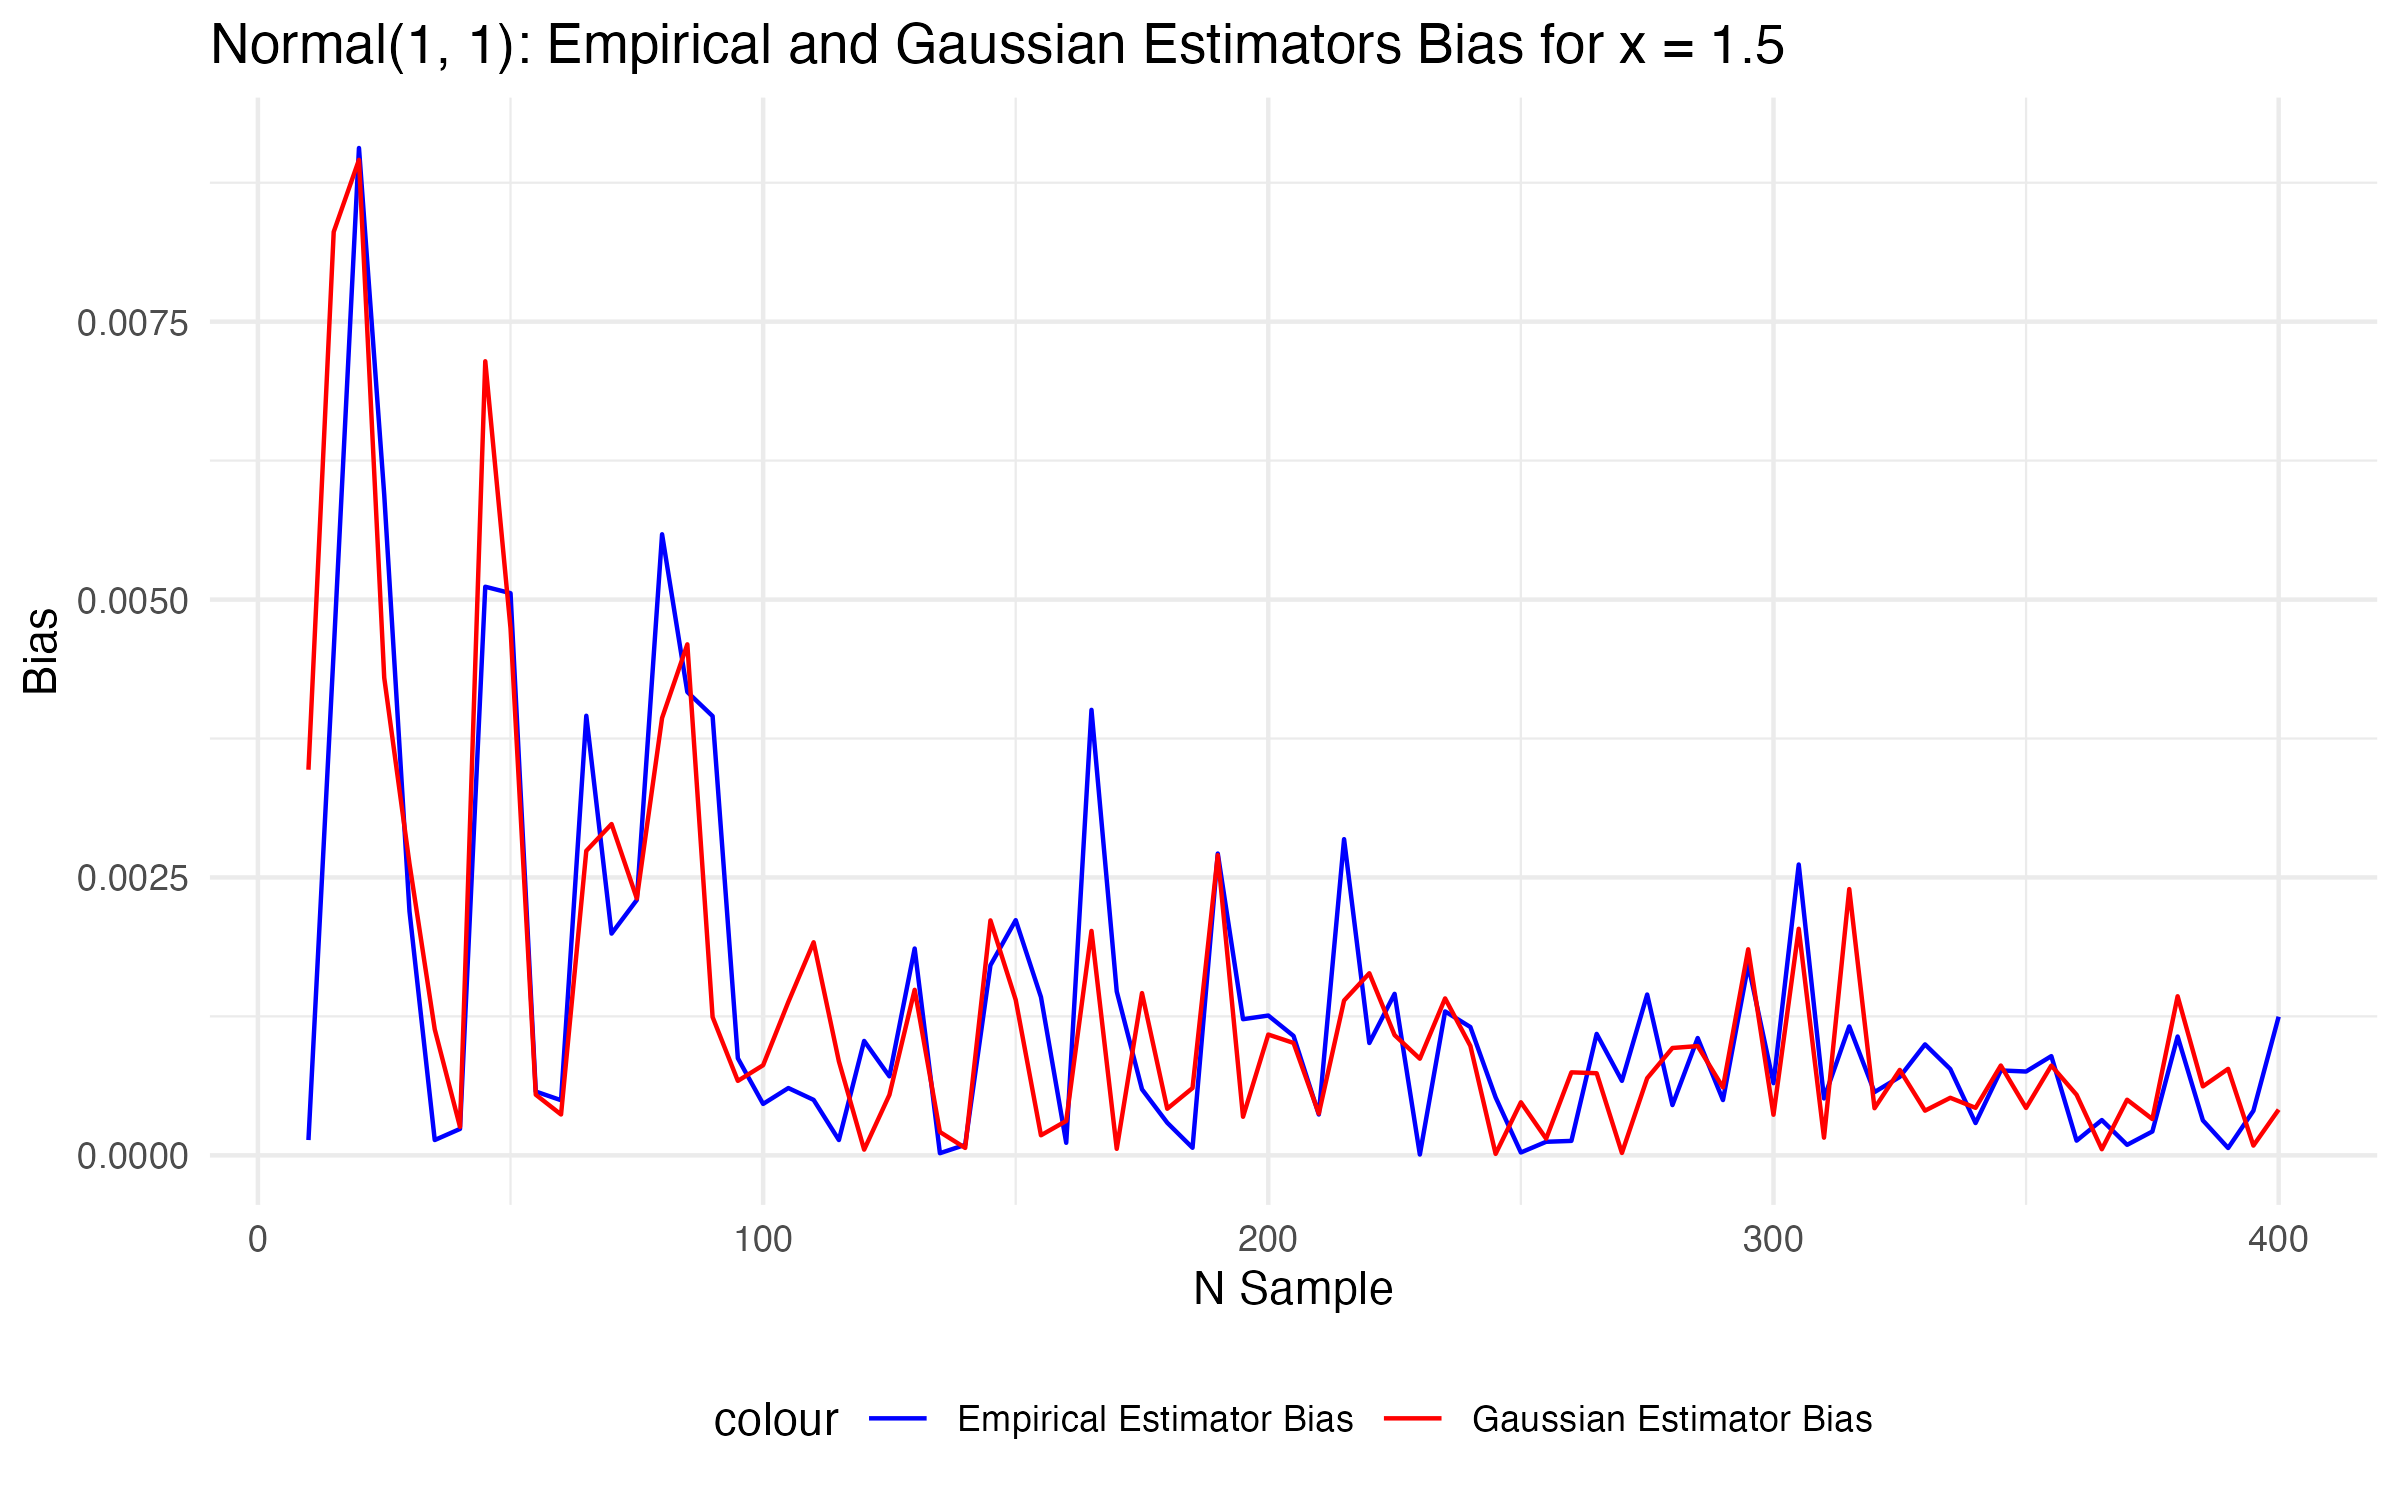
\includegraphics[width=115px]{q2d-plots/bias_x15_normal.png}
  \includegraphics[width=115px]{q2d-plots/bias_x15_t_student_10.png}
  \includegraphics[width=115px]{q2d-plots/bias_x15_t_student_70.png}
  \includegraphics[width=115px]{q2d-plots/bias_x15_t_student_150.png}
  \label{fig:bias_x15}
\end{figure}

\subsubsection*{Variance for $x = 1.5$}

\begin{figure}[H]
  \centering
  \includegraphics[width=115px]{q2d-plots/variance_x15_gamma_1_1.png}
  \includegraphics[width=115px]{q2d-plots/variance_x15_gamma_3_2.png}
  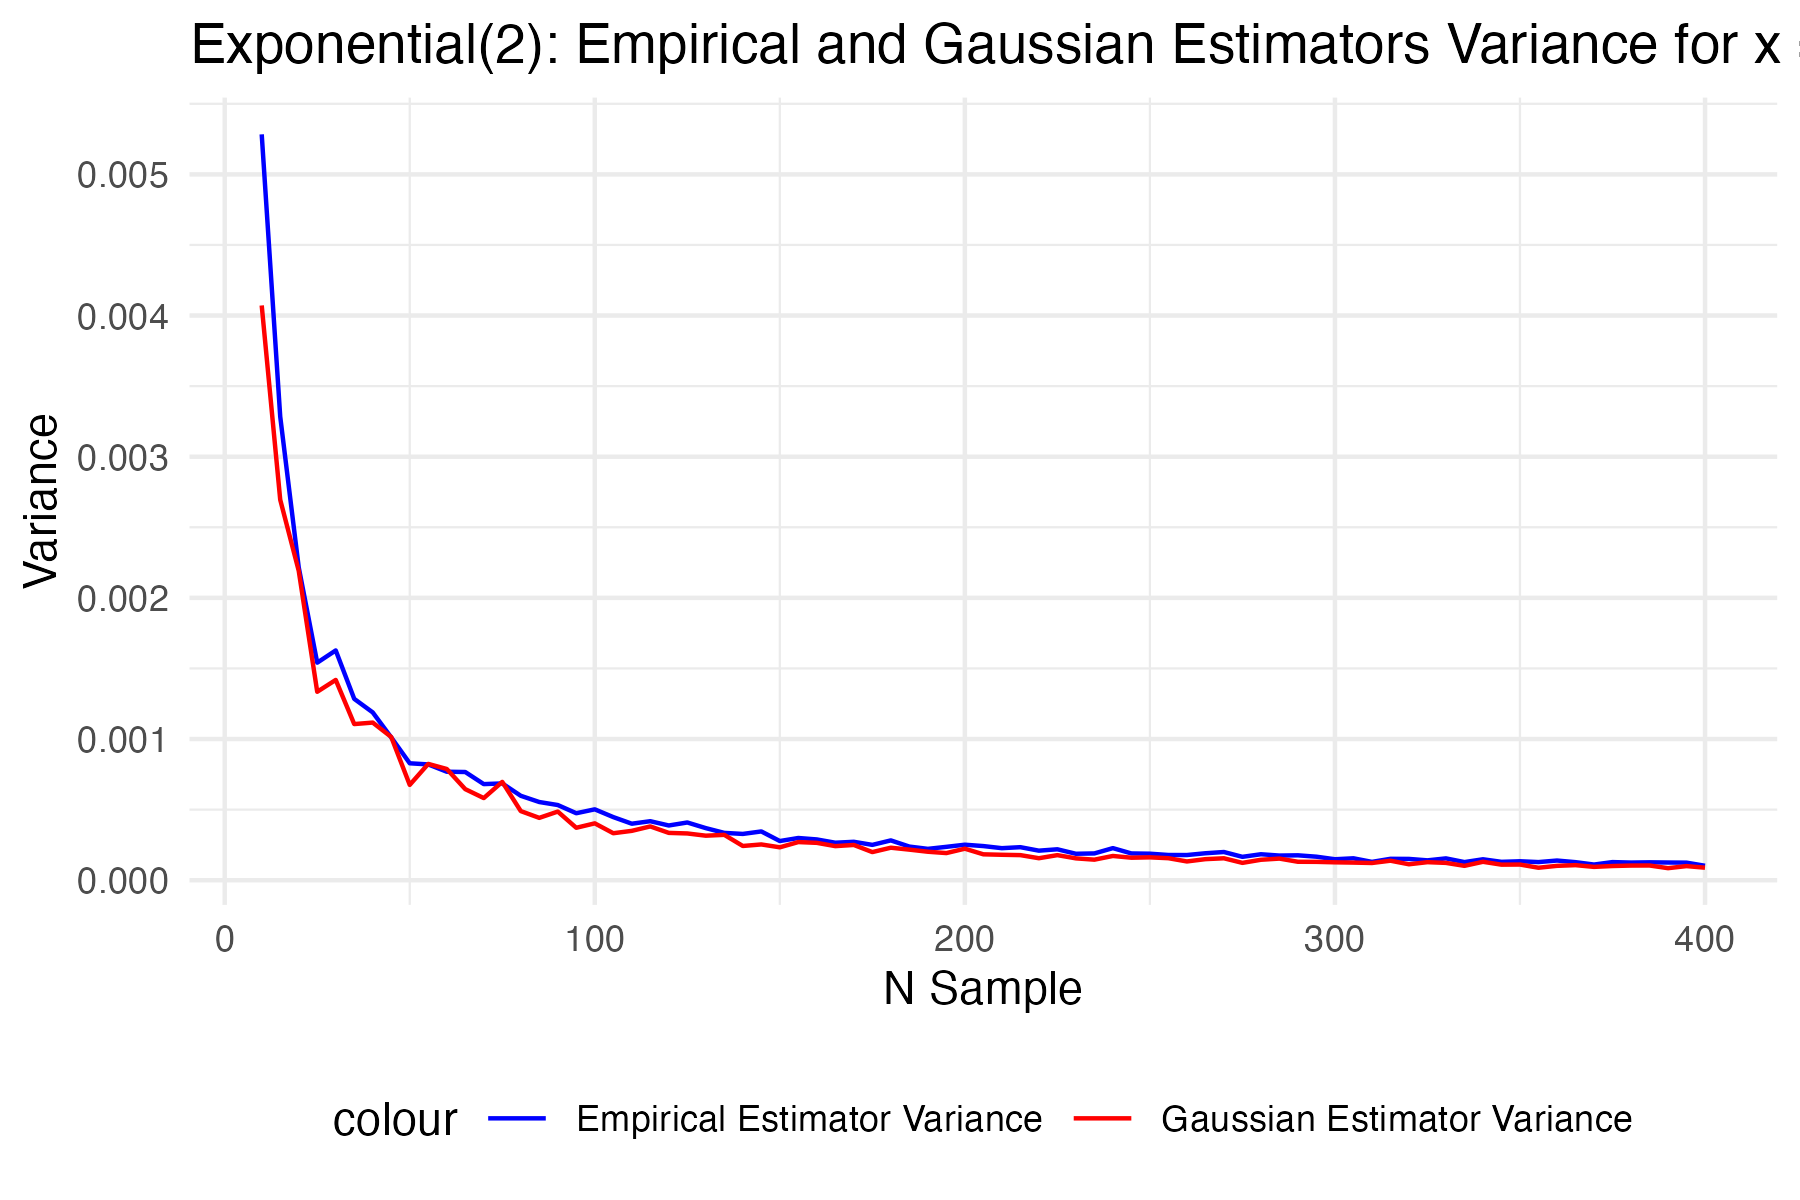
\includegraphics[width=115px]{q2d-plots/variance_x15_exponential.png}
  \includegraphics[width=115px]{q2d-plots/variance_x15_log_normal_1_1.png}
  \includegraphics[width=115px]{q2d-plots/variance_x15_log_normal_1_2.png}
  \includegraphics[width=115px]{q2d-plots/variance_x15_normal.png}
  \includegraphics[width=115px]{q2d-plots/variance_x15_t_student_10.png}
  \includegraphics[width=115px]{q2d-plots/variance_x15_t_student_70.png}
  \includegraphics[width=115px]{q2d-plots/variance_x15_t_student_150.png}
  \label{fig:variance_x15}
\end{figure}

\subsubsection*{MSE for $x = 1.5$}

\begin{figure}[H]
  \centering
  \includegraphics[width=115px]{q2d-plots/mse_x15_gamma_1_1.png}
  \includegraphics[width=115px]{q2d-plots/mse_x15_gamma_3_2.png}
  \includegraphics[width=115px]{q2d-plots/mse_x15_exponential.png}
  \includegraphics[width=115px]{q2d-plots/mse_x15_log_normal_1_1.png}
  \includegraphics[width=115px]{q2d-plots/mse_x15_log_normal_1_2.png}
  \includegraphics[width=115px]{q2d-plots/mse_x15_normal.png}
  \includegraphics[width=115px]{q2d-plots/mse_x15_t_student_10.png}
  \includegraphics[width=115px]{q2d-plots/mse_x15_t_student_70.png}
  \includegraphics[width=115px]{q2d-plots/mse_x15_t_student_150.png}
  \label{fig:mse_x15}
\end{figure}

\subsubsection*{CI for $x = 1.5$}

\begin{figure}[H]
  \centering
  \includegraphics[width=115px]{q2d-plots/ci_x15_gamma_1_1.png}
  \includegraphics[width=115px]{q2d-plots/ci_x15_gamma_3_2.png}
  \includegraphics[width=115px]{q2d-plots/ci_x15_exponential.png}
  \includegraphics[width=115px]{q2d-plots/ci_x15_log_normal_1_1.png}
  \includegraphics[width=115px]{q2d-plots/ci_x15_log_normal_1_2.png}
  \includegraphics[width=115px]{q2d-plots/ci_x15_normal.png}
  \includegraphics[width=115px]{q2d-plots/ci_x15_t_student_10.png}
  \includegraphics[width=115px]{q2d-plots/ci_x15_t_student_70.png}
  \includegraphics[width=115px]{q2d-plots/ci_x15_t_student_150.png}
  \label{fig:ci_x15}
\end{figure}

\subsubsection*{Bias for $x = 2.5$}

\begin{figure}[H]
  \centering
  \includegraphics[width=115px]{q2d-plots/bias_x25_gamma_1_1.png}
  \includegraphics[width=115px]{q2d-plots/bias_x25_gamma_3_2.png}
  \includegraphics[width=115px]{q2d-plots/bias_x25_exponential.png}
  \includegraphics[width=115px]{q2d-plots/bias_x25_log_normal_1_1.png}
  \includegraphics[width=115px]{q2d-plots/bias_x25_log_normal_1_2.png}
  \includegraphics[width=115px]{q2d-plots/bias_x25_normal.png}
  \includegraphics[width=115px]{q2d-plots/bias_x25_t_student_10.png}
  \includegraphics[width=115px]{q2d-plots/bias_x25_t_student_70.png}
  \includegraphics[width=115px]{q2d-plots/bias_x25_t_student_150.png}
  \label{fig:bias_x25}
\end{figure}

\subsubsection*{Variance for $x = 2.5$}

\begin{figure}[H]
  \centering
  \includegraphics[width=115px]{q2d-plots/variance_x25_gamma_1_1.png}
  \includegraphics[width=115px]{q2d-plots/variance_x25_gamma_3_2.png}
  \includegraphics[width=115px]{q2d-plots/variance_x25_exponential.png}
  \includegraphics[width=115px]{q2d-plots/variance_x25_log_normal_1_1.png}
  \includegraphics[width=115px]{q2d-plots/variance_x25_log_normal_1_2.png}
  \includegraphics[width=115px]{q2d-plots/variance_x25_normal.png}
  \includegraphics[width=115px]{q2d-plots/variance_x25_t_student_10.png}
  \includegraphics[width=115px]{q2d-plots/variance_x25_t_student_70.png}
  \includegraphics[width=115px]{q2d-plots/variance_x25_t_student_150.png}
  \label{fig:variance_x25}
\end{figure}

\subsubsection*{MSE for $x = 2.5$}

\begin{figure}[H]
  \centering
  \includegraphics[width=115px]{q2d-plots/mse_x25_gamma_1_1.png}
  \includegraphics[width=115px]{q2d-plots/mse_x25_gamma_3_2.png}
  \includegraphics[width=115px]{q2d-plots/mse_x25_exponential.png}
  \includegraphics[width=115px]{q2d-plots/mse_x25_log_normal_1_1.png}
  \includegraphics[width=115px]{q2d-plots/mse_x25_log_normal_1_2.png}
  \includegraphics[width=115px]{q2d-plots/mse_x25_normal.png}
  \includegraphics[width=115px]{q2d-plots/mse_x25_t_student_10.png}
  \includegraphics[width=115px]{q2d-plots/mse_x25_t_student_70.png}
  \includegraphics[width=115px]{q2d-plots/mse_x25_t_student_150.png}
  \label{fig:mse_x25}
\end{figure}

\subsubsection*{CI for $x = 2.5$}


\begin{figure}[H]
  \centering
  \includegraphics[width=115px]{q2d-plots/ci_x25_gamma_1_1.png}
  \includegraphics[width=115px]{q2d-plots/ci_x25_gamma_3_2.png}
  \includegraphics[width=115px]{q2d-plots/ci_x25_exponential.png}
  \includegraphics[width=115px]{q2d-plots/ci_x25_log_normal_1_1.png}
  \includegraphics[width=115px]{q2d-plots/ci_x25_log_normal_1_2.png}
  \includegraphics[width=115px]{q2d-plots/ci_x25_normal.png}
  \includegraphics[width=115px]{q2d-plots/ci_x25_t_student_10.png}
  \includegraphics[width=115px]{q2d-plots/ci_x25_t_student_70.png}
  \includegraphics[width=115px]{q2d-plots/ci_x25_t_student_150.png}
  \label{fig:ci_x25}
\end{figure}
}

\begin{figure}[H]
\begin{colorparagraph}{questioncolor}

\rule{\textwidth}{0.5pt}
Now we turn to estimating the density \( f(x) \). The density is the derivative of the cdf, and therefore is given by
\[
f(x) = F'(x) = \lim_{h \to 0} \frac{F(x + h) - F(x)}{h}
\]
\end{colorparagraph}

\begin{colorparagraph}{questioncolor}
\label{q2e}
\subsection{Plug-In Estimator}
(e) Use (1) and (2), for a fixed \( h \), to give a plug-in estimator for \( f(x) \) denoted \( \hat{f}(x) \).

\rule{\textwidth}{0.5pt}
\end{colorparagraph}

We aim to construct a plug-in estimator \( \hat{f}(x) \) for the density \( f(x) \) using the definition of the density as the derivative of the cumulative distribution function:
\end{figure}

\[
f(x) = F'(x) = \lim_{h \to 0} \frac{F(x + h) - F(x)}{h}.
\]

For a fixed small \( h > 0 \), we approximate \( f(x) \) by:

\[
f(x) \approx \frac{F(x + h) - F(x)}{h}.
\]

Using the empirical distribution function \( \hat{F}(x) \), the plug-in estimator \( \hat{f}(x) \) becomes:

\[
\hat{f}(x) = \frac{\hat{F}(x + h) - \hat{F}(x)}{h}.
\]

Substituting the expression for \( \hat{F}(x) \), we get:

\[
\begin{aligned}
\hat{f}(x) &= \frac{1}{h} \left( \frac{1}{n} \sum_{i=1}^n 1\{ x_i \leq x + h \} - \frac{1}{n} \sum_{i=1}^n 1\{ x_i \leq x \} \right) \\
&= \frac{1}{n h} \sum_{i=1}^n \left( 1\{ x_i \leq x + h \} - 1\{ x_i \leq x \} \right).
\end{aligned}
\]

Simplifying, note that \( 1\{ x_i \leq x + h \} - 1\{ x_i \leq x \} \) equals 1 if \( x < x_i \leq x + h \) and 0 otherwise. Therefore, the estimator counts the number of observations falling in the interval \( (x, x + h] \):

\[
\hat{f}(x) = \frac{1}{n h} \sum_{i=1}^n 1\{ x < x_i \leq x + h \} = \frac{n_h(x)}{n h},
\]

where \( n_h(x) \) is the number of observations in \( (x, x + h] \).

Thus, the plug-in estimator for \( f(x) \) is:

\[
\hat{f}(x) = \frac{1}{n h} \sum_{i=1}^n 1\{ x < x_i \leq x + h \}.
\]

\begin{figure}[H]
\begin{colorparagraph}{questioncolor}
\label{q2f}
\rule{\textwidth}{0.5pt}
\subsection{Bias of the Estimator}
(f) For fixed \( h \), compute the bias of \( \hat{f}(x) \). Prove that the bias vanishes as \( h \to 0 \).

\rule{\textwidth}{0.5pt}
\end{colorparagraph}

To compute the bias of \( \hat{f}(x) \) for fixed \( h \), we start by finding its expected value:
\end{figure}

\[
\begin{aligned}
E[\hat{f}(x)] &= E\left[ \frac{1}{n h} \sum_{i=1}^n 1\{ x < x_i \leq x + h \} \right] \\
&= \frac{1}{h} E\left[ 1\{ x < X \leq x + h \} \right] \\
&= \frac{1}{h} \left[ F(x + h) - F(x) \right].
\end{aligned}
\]

Using a Taylor series expansion of \( F(x + h) \) around \( x \):

\[
F(x + h) = F(x) + f(x) h + \frac{1}{2} f'(x) h^2 + o(h^2).
\]

Subtracting \( F(x) \) and dividing by \( h \):

\[
\frac{F(x + h) - F(x)}{h} = f(x) + \frac{1}{2} f'(x) h + o(h).
\]

Therefore, the expected value of \( \hat{f}(x) \) is:

\[
E[\hat{f}(x)] = f(x) + \frac{1}{2} f'(x) h + o(h).
\]

The bias of \( \hat{f}(x) \) is:

\[
\text{Bias}[\hat{f}(x)] = E[\hat{f}(x)] - f(x) = \frac{1}{2} f'(x) h + o(h).
\]

As \( h \to 0 \), the bias approaches zero:

\[
\lim_{h \to 0} \text{Bias}[\hat{f}(x)] = \lim_{h \to 0} \left( \frac{1}{2} f'(x) h + o(h) \right) = 0.
\]

Thus, the bias of \( \hat{f}(x) \) vanishes as \( h \to 0 \).

% In a more informal way, it is interesting to view the bias as:

% \begin{align*}
%   \mathbb{E}[\hat{f}(x) - f(x)] &=
%   \mathbb{E}\left[\frac{\hat{F}(x + h) - \hat{F}(x)}{h}\right]
%   - \mathbb{E}\left[\frac{F(x + h) - F(x)}{h}\right] \\
%   &=
%   \mathbb{E}\left[\frac{\hat{F}(x + h)}{h}\right]
%   - \mathbb{E}\left[\frac{F(x + h)}{h}\right] \quad \text{(from the results of 2.e)}\\
%   &=
%   \frac{1}{h} \left(
%     \mathbb{E}\left[\hat{F}(x + h)\right]
%     - \mathbb{E}\left[F(x + h)\right]
%   \right)
%   \\
%   &=
%   \frac{1}{h} \left(
%     \mathbb{E}\left[
%       \frac{1}{n}\sum_i^n1 \{ x_i < x + h \}
%     \right]
%     - F(x + h)
%   \right)
%   \\
%   &=
%   \frac{1}{h} \left(
%     \frac{1}{n}
%     \left[
%       \sum_i^n \mathbb{E}[1 \{ x_i \leq x \} + 1 \{ x < x_i \leq x + h \}]
%     \right]
%     - \mathbb{P}(X \leq x + h)
%   \right)
%   \\
%   &=
%   \frac{1}{h} \left(
%     \frac{1}{n}
%     \left[
%       \sum_i^n \left(\mathbb{E}[1 \{ x_i \leq x \}] + \mathbb{E}[1 \{ x < x_i \leq x + h \}]\right)
%     \right]
%     - \mathbb{P}(X \leq x + h)
%   \right)
%   \\
%   &=
%   \frac{1}{h} \left(
%     \mathbb{P}(X < x) + \frac{n_h}{n}
%     - \mathbb{P}(X \leq x + h)
%   \right)
%   \\
%   &=
%   \frac{1}{h} \left(
%     \frac{n_h}{n}
%     - \mathbb{P}(x < X \leq x + h)
%   \right)
% \end{align*}

% Thus,

% $$
% \lim_{h \to 0} \frac{1}{h} \left(
%     \frac{n_h}{n}
%     - \mathbb{P}(x < X \leq x + h)
%   \right) = 0
% $$

% \ifthenelse{\boolean{showcomments}}{
%   \begin{colorparagraph}{tacolor}CHECK:
%   Is it worth to keep this last part?
%   \end{colorparagraph}
% }

\begin{figure}[H]
\begin{colorparagraph}{questioncolor}
\label{q2g}
\rule{\textwidth}{0.5pt}
\subsection{Bias Order}
(g) Assume that \( f(x) \) is twice continuously differentiable. Prove that the bias of \( \hat{f}(x) \) is \( O(h) \) and characterize the constant. That is, show that
\[
\mathbb{E}[\hat{f}(x) - f(x)] = Kh + o(h)
\]
and give the precise form of \( K \).

\rule{\textwidth}{0.5pt}
\end{colorparagraph}

Starting from the expression for the expected value of \( \hat{f}(x) \):
\end{figure}

\[
\mathbb{E}[\hat{f}(x)] = \frac{1}{h} \left( F(x + h) - F(x) \right).
\]

Using the Taylor expansion of \( F(x + h) \) around \( x \):

\[
F(x + h) = F(x) + f(x) h + \frac{1}{2} f'(x) h^2 + \frac{1}{6} f''(x) h^3 + o(h^3).
\]

Subtracting \( F(x) \) and dividing by \( h \):

\[
\frac{F(x + h) - F(x)}{h} = f(x) + \frac{1}{2} f'(x) h + \frac{1}{6} f''(x) h^2 + o(h^2).
\]

Therefore, the expected value of \( \hat{f}(x) \) is:

\[
\mathbb{E}[\hat{f}(x)] = f(x) + \frac{1}{2} f'(x) h + o(h).
\]

The bias of \( \hat{f}(x) \) is:

\[
\mathbb{E}[\hat{f}(x) - f(x)] = \frac{1}{2} f'(x) h + o(h).
\]

Thus, the bias is \( O(h) \), and the constant \( K \) is given by:

\[
K = \frac{1}{2} f'(x).
\]

\begin{figure}[H]
\begin{colorparagraph}{questioncolor}
\label{q2h}
\rule{\textwidth}{0.5pt}
\subsection{Variance of the Estimator}
(h) For fixed \( h \), compute the variance denoted \( \Sigma = \mathbb{V}[\hat{f}(x)] \). Provide a consistent estimator.

\rule{\textwidth}{0.5pt}
\end{colorparagraph}

We compute the variance of \( \hat{f}(x) \) for fixed \( h \). Recall that \( \hat{f}(x) \) is given by:
\end{figure}

\[
\hat{f}(x) = \frac{1}{n h} \sum_{i=1}^n 1\{ x < x_i \leq x + h \}.
\]

Define the indicator variables:

\[
Y_i = 1\{ x < x_i \leq x + h \}, \quad i = 1, 2, \dots, n.
\]

Each \( Y_i \) is an independent Bernoulli random variable with success probability:

\[
p = \mathbb{P}(x < X \leq x + h) = F(x + h) - F(x).
\]

The variance of \( \hat{f}(x) \) is:

\[
\begin{aligned}
\mathbb{V}[\hat{f}(x)] &= \mathbb{V}\left( \frac{1}{n h} \sum_{i=1}^n Y_i \right) \\
&= \frac{1}{(n h)^2} \sum_{i=1}^n \mathbb{V}[Y_i] \\
&= \frac{1}{(n h)^2} \cdot n \cdot p (1 - p) \\
&= \frac{p (1 - p)}{n h^2}.
\end{aligned}
\]

To express \( \Sigma = \mathbb{V}[\hat{f}(x)] \) in terms of \( f(x) \), we approximate \( p \) for small \( h \):

\[
\begin{aligned}
p &= F(x + h) - F(x) \\
&= \int_x^{x + h} f(t) \, dt \\
&= f(x) h + \frac{1}{2} f'(x) h^2 + o(h^2).
\end{aligned}
\]

Therefore, for small \( h \), we have \( p \approx f(x) h \). Then, \( p (1 - p) \approx f(x) h (1 - f(x) h) \approx f(x) h \), since \( h \) is small.

Substituting back into the variance:

\[
\mathbb{V}[\hat{f}(x)] \approx \frac{f(x) h}{n h^2} = \frac{f(x)}{n h}.
\]

Thus, the variance is:

\[
\Sigma = \mathbb{V}[\hat{f}(x)] = \frac{f(x)}{n h} + o\left( \frac{1}{n h} \right).
\]

To provide a consistent estimator of \( \Sigma \), we estimate \( p \) using the sample proportion:

\[
\hat{p} = \frac{1}{n} \sum_{i=1}^n Y_i = n h \hat{f}(x) \cdot \frac{1}{n} = h \hat{f}(x).
\]

Then, the estimated variance is:

\[
\begin{aligned}
\hat{\Sigma} &= \frac{\hat{p} (1 - \hat{p})}{n h^2} \\
&= \frac{h \hat{f}(x) \left( 1 - h \hat{f}(x) \right)}{n h^2} \\
&= \frac{\hat{f}(x) \left( 1 - h \hat{f}(x) \right)}{n h}.
\end{aligned}
\]

Since \( h \) is small, \( h \hat{f}(x) \) is negligible, and we can approximate:

\[
\hat{\Sigma} \approx \frac{\hat{f}(x)}{n h}.
\]

Therefore, a consistent estimator of the variance \( \Sigma \) is:

\[
\hat{\Sigma} = \frac{\hat{f}(x)}{n h}.
\]

\begin{figure}[H]
\begin{colorparagraph}{questioncolor}
\label{q2i}
\rule{\textwidth}{0.5pt}
\subsection{Mean Square Error}
(i) Compute the mean square error of your estimator and find the value of \( h \) that minimizes it. Characterize precisely what happens to this optimal \( h \) as \( n \to \infty \). How would you choose \( h \) in an application for the goal of estimation?

\rule{\textwidth}{0.5pt}
\end{colorparagraph}

The mean square error (MSE) of the estimator \( \hat{f}(x) \) is given by the sum of the squared bias and the variance:
\end{figure}

\[
\text{MSE}(h) = \left( \mathbb{E}[\hat{f}(x)] - f(x) \right)^2 + \mathbb{V}[\hat{f}(x)].
\]

From previous results, the bias is approximately:

\[
\text{Bias} = \mathbb{E}[\hat{f}(x)] - f(x) = \frac{1}{2} f'(x) h + o(h).
\]

The variance is approximately:

\[
\mathbb{V}[\hat{f}(x)] = \frac{f(x)}{n h} + o\left( \frac{1}{n h} \right).
\]

Ignoring higher-order terms, the MSE becomes:

\[
\text{MSE}(h) = \left( \frac{1}{2} f'(x) h \right)^2 + \frac{f(x)}{n h} = \frac{1}{4} [f'(x)]^2 h^2 + \frac{f(x)}{n h}.
\]

To find the value of \( h \) that minimizes the MSE, take the derivative of \( \text{MSE}(h) \) with respect to \( h \) and set it equal to zero:

\[
\frac{d}{d h} \text{MSE}(h) = \frac{1}{2} [f'(x)]^2 h - \frac{f(x)}{n h^2} = 0.
\]

Solving for \( h \):

\[
\frac{1}{2} [f'(x)]^2 h = \frac{f(x)}{n h^2},
\]

\[
\frac{1}{2} [f'(x)]^2 n h^3 = f(x),
\]

\[
h^3 = \frac{2 f(x)}{[f'(x)]^2 n}.
\]

Therefore, the optimal bandwidth \( h \) that minimizes the MSE is:

\[
h_{\text{opt}} = \left( \frac{2 f(x)}{[f'(x)]^2 n} \right)^{1/3}.
\]

As \( n \to \infty \), the optimal \( h \) behaves like:

\[
h_{\text{opt}} \propto n^{-1/3}.
\]

This means that the optimal bandwidth decreases at the rate of \( n^{-1/3} \) as the sample size increases.

In an application aiming for estimation, we should choose \( h \) proportional to \( n^{-1/3} \) to balance the bias and variance, minimizing the MSE. Specifically:

\[
h = C n^{-1/3},
\]

where \( C \) is a constant that may depend on estimates of \( f(x) \) and \( f'(x) \). Since \( f(x) \) and \( f'(x) \) are typically unknown, we can use pilot estimates or assume reasonable values based on prior knowledge to select \( h \).

\begin{figure}[H]
\begin{colorparagraph}{questioncolor}
\label{q2j}
\rule{\textwidth}{0.5pt}
\subsection{Asymptotic Normality for Fixed \( h \)}
(j) For fixed \( h \), prove that
\[
\frac{\hat{f}(x) - \mathbb{E}[\hat{f}(x)]}{\Sigma^{1/2}} \to_d \mathcal{N}(0, 1).
\]

\rule{\textwidth}{0.5pt}
\end{colorparagraph}

Recall that:
\end{figure}

\[
\hat{f}(x) = \frac{1}{n h} \sum_{i=1}^n Y_i,
\]

with \( Y_i = 1\{ x < x_i \leq x + h \} \). The \( Y_i \) are independent and identically distributed (i.i.d.) Bernoulli random variables with success probability:

\[
p = \mathbb{P}(x < X \leq x + h) = F(x + h) - F(x).
\]

The mean and variance of \( Y_i \) are:

\[
\mathbb{E}[Y_i] = p, \quad \mathbb{V}[Y_i] = p (1 - p).
\]

The expected value and variance of \( \hat{f}(x) \) are:

\[
\mathbb{E}[\hat{f}(x)] = \frac{1}{n h} \sum_{i=1}^n \mathbb{E}[Y_i] = \frac{p}{h},
\]

\[
\mathbb{V}[\hat{f}(x)] = \frac{1}{(n h)^2} \sum_{i=1}^n \mathbb{V}[Y_i] = \frac{p (1 - p)}{n h^2} = \Sigma.
\]

Define the standardized version of \( \hat{f}(x) \):

\[
Z_n = \frac{\hat{f}(x) - \mathbb{E}[\hat{f}(x)]}{\Sigma^{1/2}} = \frac{\frac{1}{n h} \sum_{i=1}^n Y_i - \frac{p}{h}}{\left( \frac{p (1 - p)}{n h^2} \right)^{1/2}} = \frac{\sum_{i=1}^n (Y_i - p)}{\sqrt{n p (1 - p)}}.
\]

Since the \( Y_i \) are i.i.d. with finite variance, by the Central Limit Theorem:

\[
\frac{\sum_{i=1}^n (Y_i - p)}{\sqrt{n p (1 - p)}} \xrightarrow{d} \mathcal{N}(0, 1).
\]

Therefore,

\[
\frac{\hat{f}(x) - \mathbb{E}[\hat{f}(x)]}{\Sigma^{1/2}} \xrightarrow{d} \mathcal{N}(0, 1).
\]

\begin{figure}[H]
\begin{colorparagraph}{questioncolor}
\label{q2k}
\rule{\textwidth}{0.5pt}
\subsection{Sufficient Conditions for Asymptotic Normality}
(k) Provide sufficient conditions so that
\[
\frac{\hat{f}(x) - f(x)}{\Sigma^{1/2}} \to_d \mathcal{N}(0, 1).
\]
Characterize precisely the requirements that \( h \) must obey as \( n \to \infty \).

\rule{\textwidth}{0.5pt}
\end{colorparagraph}

We are to provide sufficient conditions such that:
\end{figure}

\[
\frac{\hat{f}(x) - f(x)}{\Sigma^{1/2}} \xrightarrow{d} \mathcal{N}(0, 1),
\]

where \(\Sigma = \mathbb{V}[\hat{f}(x)]\).

From earlier results:

The bias of \(\hat{f}(x)\) is approximately:

\[
\mathbb{E}[\hat{f}(x)] - f(x) = \frac{1}{2} f'(x) h + o(h).
\]

The variance of \(\hat{f}(x)\) is approximately:

\[
\Sigma = \mathbb{V}[\hat{f}(x)] = \frac{f(x)}{n h} + o\left( \frac{1}{n h} \right).
\]

The standard deviation is:

\[
\Sigma^{1/2} = \sqrt{\frac{f(x)}{n h}} + o\left( \sqrt{\frac{1}{n h}} \right).
\]

To ensure that the standardized estimator converges in distribution to a standard normal, the bias must be negligible compared to the standard deviation. Specifically, we require:

\[
\frac{\mathbb{E}[\hat{f}(x)] - f(x)}{\Sigma^{1/2}} \to 0 \quad \text{as } n \to \infty.
\]

Computing the standardized bias:

\[
\begin{aligned}
\frac{\mathbb{E}[\hat{f}(x)] - f(x)}{\Sigma^{1/2}} &\approx \frac{\frac{1}{2} f'(x) h}{\sqrt{\dfrac{f(x)}{n h}}} \\
&= \frac{1}{2} f'(x) h \cdot \sqrt{\frac{n h}{f(x)}} \\
&= \frac{1}{2} \frac{f'(x)}{\sqrt{f(x)}} \sqrt{n h^3}.
\end{aligned}
\]

Therefore, to have the standardized bias tend to zero, we need:

\[
\sqrt{n h^3} \to 0 \quad \text{as } n \to \infty.
\]

This implies:

\[
n h^3 \to 0 \quad \text{as } n \to \infty.
\]

At the same time, to ensure that the variance \(\Sigma\) shrinks to zero (i.e., the estimator becomes more precise), we require:

\[
n h \to \infty \quad \text{as } n \to \infty.
\]

In summary, the sufficient conditions are:

\begin{itemize}
    \item \( h \to 0 \) as \( n \to \infty \),
    \item \( n h \to \infty \) as \( n \to \infty \),
    \item \( n h^3 \to 0 \) as \( n \to \infty \).
\end{itemize}

Characterizing the Requirements on \( h \):

Let us consider \( h \) of the form:

\[
h = n^{-\beta},
\]

for some \( \beta > 0 \).

We analyze the conditions:

1. \( h \to 0 \):

\[
h = n^{-\beta} \to 0 \quad \text{if } \beta > 0.
\]

2. \( n h = n \cdot n^{-\beta} = n^{1 - \beta} \to \infty \):

\[
n h \to \infty \quad \text{if } 1 - \beta > 0 \quad \text{or} \quad \beta < 1.
\]

3. \( n h^3 = n \cdot n^{-3\beta} = n^{1 - 3\beta} \to 0 \):

\[
n h^3 \to 0 \quad \text{if } 1 - 3\beta < 0 \quad \text{or} \quad \beta > \frac{1}{3}.
\]

Combining these conditions, we require:

\[
\frac{1}{3} < \beta < 1.
\]

Therefore, choosing \( h \) such that:

\[
h = n^{-\beta}, \quad \text{with} \quad \beta \in \left( \frac{1}{3}, 1 \right),
\]

satisfies all the sufficient conditions.

Thus, For the asymptotic normality:

\[
\frac{\hat{f}(x) - f(x)}{\Sigma^{1/2}} \xrightarrow{d} \mathcal{N}(0, 1),
\]

to hold, it is sufficient that:

\begin{itemize}
    \item The bandwidth \( h \) decreases to zero at a rate \( h = n^{-\beta} \) with \( \beta \in \left( \frac{1}{3}, 1 \right) \).
    \item This ensures \( h \to 0 \), \( n h \to \infty \), and \( n h^3 \to 0 \) as \( n \to \infty \).
\end{itemize}

\begin{figure}[H]
\begin{colorparagraph}{questioncolor}
\label{q2l}
\rule{\textwidth}{0.5pt}
\subsection{Comparison of Requirements for \( h \)}
(l) Compare the requirements on \( h \) in part (k) to what you found in part (i). Discuss what you find. How would you choose \( h \) in an application for the goal of inference?

\rule{\textwidth}{0.5pt}
\end{colorparagraph}

In part (i), we found that the bandwidth \( h \) that minimizes the mean square error (MSE) of the estimator \( \hat{f}(x) \) is:
\end{figure}

\[
h_{\text{opt}} = \left( \frac{2 f(x)}{[f'(x)]^2 n} \right)^{1/3} \propto n^{-1/3}.
\]

This implies that to minimize the MSE, we should choose \( h \) proportional to \( n^{-1/3} \).

In part (k), we determined sufficient conditions for the asymptotic normality of the standardized estimator:

\[
\frac{\hat{f}(x) - f(x)}{\Sigma^{1/2}} \xrightarrow{d} \mathcal{N}(0, 1),
\]

which require that:

\begin{itemize}
    \item \( h \to 0 \) as \( n \to \infty \),
    \item \( n h \to \infty \) as \( n \to \infty \),
    \item \( n h^3 \to 0 \) as \( n \to \infty \).
\end{itemize}

These conditions are satisfied when \( h = n^{-\beta} \) with \( \beta \) in the interval \( \left( \frac{1}{3}, 1 \right) \).

Comparing these results, we observe that:

\begin{itemize}
    \item The optimal \( h \) for minimizing MSE is \( h_{\text{opt}} \propto n^{-1/3} \), which corresponds to \( \beta = \frac{1}{3} \).
    \item The asymptotic normality requires \( \beta > \frac{1}{3} \).
\end{itemize}

This indicates a trade-off between bias and variance:

\begin{itemize}
    \item Choosing \( h \) proportional to \( n^{-1/3} \) minimizes the MSE but does not satisfy the condition \( n h^3 \to 0 \), since \( n h^3 = n \cdot (n^{-1/3})^3 = 1 \), which does not converge to zero.
    \item To achieve asymptotic normality for inference purposes, we need \( h \) to decrease slightly faster than \( n^{-1/3} \), i.e., \( h \propto n^{-\beta} \) with \( \beta > \frac{1}{3} \).
\end{itemize}

In practice, when the goal is estimation (minimizing MSE), we might choose \( h \propto n^{-1/3} \). However, for inference (e.g., constructing confidence intervals), we need the standardized estimator to be asymptotically normal. Therefore, we should choose \( h \) such that:

\[
h = n^{-\beta}, \quad \text{with} \quad \beta \in \left( \frac{1}{3}, 1 \right).
\]

By selecting \( \beta \) slightly greater than \( \frac{1}{3} \), we ensure that:

\begin{itemize}
    \item The bias becomes negligible compared to the standard deviation.
    \item The conditions \( n h \to \infty \) and \( n h^3 \to 0 \) are satisfied.
\end{itemize}

This choice balances the need for the estimator to be asymptotically normal (which facilitates valid statistical inference) while controlling the bias and variance.

The optimal choice for \( h \) is:

\[
h = n^{-\beta}, \quad \text{where} \quad \beta = \frac{1}{3} + \varepsilon, \quad \varepsilon > 0.
\]

This ensures that the standardized estimator converges in distribution to a normal distribution, enabling us to construct confidence intervals and perform hypothesis tests reliably.

\begin{figure}[H]
\begin{colorparagraph}{questioncolor}
\label{q2m}
\rule{\textwidth}{0.5pt}
\subsection{Simulation Study on Empirical Performance}
(m) Conduct a simulation study to examine the empirical performance of \( \hat{f}(x) \). Evaluate the bias and variance of your estimator and the quality of the Normal approximation. Compute the empirical coverage and length of 95\% confidence intervals. Study what happens as you vary \( n \), \( h \), the true distribution, and the evaluation point \( x \).

\rule{\textwidth}{0.5pt}
\end{colorparagraph}

For this question, we use the following calculations:
\end{figure}

$$
p_{x, h} = \frac{n_h}{n}, \quad \text{where} \ n_h \ \text{is the n. of obs in} \ h \text{and} \ n \text{is the n. of obs in the sample simulation}
$$

$$
\hat{f}(x)_h = \frac{p_{x, h}}{h} 
$$

$$
\text{Var}[\hat{f}(x)_h] = \frac{p_{x, h} (1 - p_{x, h})}{n h^2} = \hat{\sigma}^2_{x, h}
$$

$$
\text{CI} = \left[
  \hat{f}(x)_h - t_{n-1}\left(1 - \frac{\alpha}{2}\right) \hat{\sigma}_{x, h},
  \quad \hat{f}(x)_h + t_{n-1}\left(1 - \frac{\alpha}{2}\right) \hat{\sigma}_{x, h}
\right]
$$

We run simulations using:
\begin{itemize}
  \item Sample sizes $n$ of: 10, 25, 50, 75, 100, 200, 300, 400, 500, 600, 700, 800, 900, 1000
  \item Interval $h$ of:
  $$
  h_i = \frac{1}{n_i^{1/3}} + \varepsilon \quad \ \text{for} \ n_i \ \text{in sample sizes available and} \ \varepsilon = 0.0001 
  $$
  The intervals tested coincide with the optimal values found for the previous solutions.
  \item The following distributions:
  \begin{itemize}
    \item T-Student(30)
    \item T-Student(50)
    \item T-Student(100)
    \item Normal(0, 1)
    \item Normal(1, 1)
    \item Gamma(1, 1)
    \item Gamma(2, 3)
    \item Log-Normal(1, 1)
  \end{itemize}
  \item 1000 simulations for every combination of $n$, $h$ and distribution, using the results for $x = 0.5$ and $x = 1$, totaling 1.792 million simulations.
\end{itemize}

We check the performance of the results based on the efficiency of the CI.

Given that we always use CI of $95\%$, we hope that in $95\%$ of the simulations the true $f(x)$ falls within the ranges determined.

Our results agree with the theoretical conclusions: for smaller samples, bigger $h$ yields more precise results. As $n$ increases, the results using bigger $h$ has a considerable decrease in performance.

The best results, as expected, are found for big $n$ and, on average, $h = \frac{1}{n^{1/3}}$, as specified to provide good inference.

\ifthenelse{\boolean{imagesbool:q2m}}{
\begin{table}[H]
  \centering
  \title{$f(x)$ Simulation Results for T-Student(30) in $x = 1$}
  \input{q2m-data/simulations_f_x10_t_student_30_comp_h_n.tex}
  \label{tab:simulation_t_student_30_x10}
\end{table}

\begin{table}[H]
  \centering
  \title{$f(x)$ Simulation Results for T-Student(50) in $x = 1$}
  \input{q2m-data/simulations_f_x10_t_student_50_comp_h_n.tex}
  \label{tab:simulation_t_student_50_x10}
\end{table}

\begin{table}[H]
  \centering
  \title{$f(x)$ Simulation Results for T-Student(100) in $x = 1$}
  \input{q2m-data/simulations_f_x10_t_student_100_comp_h_n.tex}
  \label{tab:simulation_t_student_100_x10}
\end{table}

\begin{table}[H]
  \centering
  \title{$f(x)$ Simulation Results for Normal(0,1) in $x = 1$}
  \input{q2m-data/simulations_f_x10_normal_0_1_comp_h_n.tex}
  \label{tab:simulation_normal_0_1_x10}
\end{table}

\begin{table}[H]
  \centering
  \title{$f(x)$ Simulation Results for Normal(1,1) in $x = 1$}
  \input{q2m-data/simulations_f_x10_normal_1_1_comp_h_n.tex}
  \label{tab:simulation_normal_1_1_x10}
\end{table}

\begin{table}[H]
  \centering
  \title{$f(x)$ Simulation Results for Gamma(1,1) in $x = 1$}
  \input{q2m-data/simulations_f_x10_gamma_1_1_comp_h_n.tex}
  \label{tab:simulation_gamma_1_1_x10}
\end{table}

\begin{table}[H]
  \centering
  \title{$f(x)$ Simulation Results for Gamma(2,3) in $x = 1$}
  \input{q2m-data/simulations_f_x10_gamma_2_3_comp_h_n.tex}
  \label{tab:simulation_gamma_2_3_x10}
\end{table}

\begin{table}[H]
  \centering
  \title{$f(x)$ Simulation Results for Log-Normal(1,1) in $x = 1$}
  \input{q2m-data/simulations_f_x10_log_normal_1_1_comp_h_n.tex}
  \label{tab:simulation_log_normal_1_1_x10}
\end{table}

\begin{table}[H]
  \centering
  \title{$f(x)$ Simulation Results for T-Student(30) in $x = 0.5$}
  \input{q2m-data/simulations_f_x5_t_student_30_comp_h_n.tex}
  \label{tab:simulation_t_student_30_x5}
\end{table}

\begin{table}[H]
  \centering
  \title{$f(x)$ Simulation Results for T-Student(50) in $x = 0.5$}
  \input{q2m-data/simulations_f_x5_t_student_50_comp_h_n.tex}
  \label{tab:simulation_t_student_50_x5}
\end{table}

\begin{table}[H]
  \centering
  \title{$f(x)$ Simulation Results for T-Student(100) in $x = 0.5$}
  \input{q2m-data/simulations_f_x5_t_student_100_comp_h_n.tex}
  \label{tab:simulation_t_student_100_x5}
\end{table}

\begin{table}[H]
  \centering
  \title{$f(x)$ Simulation Results for Normal(0,1) in $x = 0.5$}
  \input{q2m-data/simulations_f_x5_normal_0_1_comp_h_n.tex}
  \label{tab:simulation_normal_0_1_x5}
\end{table}

\begin{table}[H]
  \centering
  \title{$f(x)$ Simulation Results for Normal(1,1) in $x = 0.5$}
  \input{q2m-data/simulations_f_x5_normal_1_1_comp_h_n.tex}
  \label{tab:simulation_normal_1_1_x5}
\end{table}

\begin{table}[H]
  \centering
  \title{$f(x)$ Simulation Results for Gamma(1,1) in $x = 0.5$}
  \input{q2m-data/simulations_f_x5_gamma_1_1_comp_h_n.tex}
  \label{tab:simulation_gamma_1_1_x5}
\end{table}

\begin{table}[H]
  \centering
  \title{$f(x)$ Simulation Results for Gamma(2,3) in $x = 0.5$}
  \input{q2m-data/simulations_f_x5_gamma_2_3_comp_h_n.tex}
  \label{tab:simulation_gamma_2_3_x5}
\end{table}

\begin{table}[H]
  \centering
  \title{$f(x)$ Simulation Results for Log-Normal(1,1) in $x = 0.5$}
  \input{q2m-data/simulations_f_x5_log_normal_1_1_comp_h_n.tex}
  \label{tab:simulation_log_normal_1_1_x5}
\end{table}
}

\begin{figure}[H]
\begin{colorparagraph}{questioncolor}

\rule{\textwidth}{0.5pt}
\label{q3}
\section{Application}

The file \texttt{Banerji-Berry-Shotland\_2017\_AEJ.csv} contains data from a recent paper.

The outcome is a (normalized) child's test, in \texttt{caser\_total\_norm}. \texttt{treatment} has four different values, indicating different trainings for mothers. The first is the baseline/control. There are six \( X \) variables (dummies) and three \( W \) variables (continuous). We want to explore the impact of each treatment relative to the baseline (\texttt{treatment}=1).

\rule{\textwidth}{0.5pt}
\end{colorparagraph}

\begin{colorparagraph}{questioncolor}
\section*{LASSO \& Discrete Heterogeneity}
\label{q3a}
\rule{\textwidth}{0.5pt}
\subsection{Run a Single Regression}
(a) Run a single linear regression that provides estimates and inference for \( \mu_t = \mathbb{E}[Y(t)] \), \( t = 1, 2, 3, 4 \). Add covariates to the regression to see if efficiency is improved. First add the covariates directly and then do it demeaned and interacted. Try adding interactions among the \( X \) and \( W \).

\rule{\textwidth}{0.5pt}
\end{colorparagraph}
\end{figure}

\subsubsection*{Regression without Covariates}
\begin{figure}[H]
\begin{lstlisting}[style=RstyleComment, caption=Regression without Covariates]
  Call:
  lm(formula = caser_total_norm ~ ., data = banerji_data %>% select(caser_total_norm, 
      t2, t3, t4))
  
  Residuals:
      Min      1Q  Median      3Q     Max 
  -1.3966 -0.8517 -0.2407  0.7092  2.2221 
  
  Coefficients:
              Estimate Std. Error t value Pr(>|t|)    
  (Intercept)  0.18733    0.01643  11.403  < 2e-16 ***
  t2           0.05233    0.02325   2.250 0.024434 *  
  t3           0.07789    0.02353   3.310 0.000936 ***
  t4           0.10038    0.02331   4.307 1.66e-05 ***
  ---
  Signif. codes:  0 '***' 0.001 '**' 0.01 '*' 0.05 '.' 0.1 ' ' 1
  
  Residual standard error: 0.9998 on 14570 degrees of freedom
  Multiple R-squared:  0.001408,	Adjusted R-squared:  0.001202 
  F-statistic: 6.847 on 3 and 14570 DF,  p-value: 0.0001319
\end{lstlisting}
\end{figure}

The estimators for the treatment are:
\begin{itemize}
  \item $\hat{\mu}_1 = \mathbb{E}[Y(1)] = 0.18733$
  \item $\hat{\mu}_2 = \mathbb{E}[Y(2)] = 0.18733 + 0.05233 = 0.23966$
  \item $\hat{\mu}_3 = \mathbb{E}[Y(3)] = 0.18733 + 0.07789 = 0.26522$
  \item $\hat{\mu}_4 = \mathbb{E}[Y(4)] = 0.18733 + 0.10038 = 0.28771$
\end{itemize}

All treatment are statistically different from $t_1$ (control).

\subsubsection*{Regression with Covariates}
\begin{figure}[H]
\begin{lstlisting}[style=RstyleComment, caption=Regression with Covariates]
  Call:
  lm(formula = caser_total_norm ~ ., data = banerji_data)
  
  Residuals:
      Min      1Q  Median      3Q     Max 
  -3.1702 -0.2850 -0.0686  0.2346  3.1656 
  
  Coefficients:
                       Estimate Std. Error t value Pr(>|t|)    
  (Intercept)          0.047014   0.024572   1.913  0.05573 .  
  age                  0.010872   0.002372   4.584 4.60e-06 ***
  state                0.007818   0.008483   0.922  0.35678    
  bl_caser_total_norm  0.852219   0.004639 183.720  < 2e-16 ***
  boy                  0.052580   0.007636   6.886 5.96e-12 ***
  number_of_kids      -0.008028   0.002508  -3.201  0.00137 ** 
  mother_educ          0.120762   0.011264  10.721  < 2e-16 ***
  factor_educ          0.073858   0.008155   9.057  < 2e-16 ***
  mother_age30        -0.017244   0.007926  -2.176  0.02961 *  
  farmingIncome        0.034616   0.008106   4.270 1.96e-05 ***
  t2                   0.014434   0.010533   1.370  0.17057    
  t3                   0.025175   0.010667   2.360  0.01828 *  
  t4                   0.055961   0.010569   5.295 1.21e-07 ***
  ---
  Signif. codes:  0 '***' 0.001 '**' 0.01 '*' 0.05 '.' 0.1 ' ' 1
  
  Residual standard error: 0.4525 on 14561 degrees of freedom
  Multiple R-squared:  0.7955,	Adjusted R-squared:  0.7954 
  F-statistic:  4721 on 12 and 14561 DF,  p-value: < 2.2e-16
\end{lstlisting}
\end{figure}

When adding the covariates without demeaning them, we cannot recover directly the influence of the treatment. This happens because the mean of the covariates is not zero and, thus, influences the parameters of $t_2$, $t_3$, $t_4$.

\subsubsection*{Regression with Demeaned Covariates}
\begin{figure}[H]
\begin{lstlisting}[style=RstyleComment, caption=Regression with Demeaned Covariates]
Call:
lm(formula = caser_total_norm ~ ., data = banerji_demeaned_data)

Residuals:
    Min      1Q  Median      3Q     Max 
-3.1702 -0.2850 -0.0686  0.2346  3.1656 

Coefficients:
                     Estimate Std. Error t value Pr(>|t|)    
(Intercept)          0.220804   0.007444  29.660  < 2e-16 ***
age                  0.010872   0.002372   4.584 4.60e-06 ***
state                0.007818   0.008483   0.922  0.35678    
bl_caser_total_norm  0.852219   0.004639 183.720  < 2e-16 ***
boy                  0.052580   0.007636   6.886 5.96e-12 ***
number_of_kids      -0.008028   0.002508  -3.201  0.00137 ** 
mother_educ          0.120762   0.011264  10.721  < 2e-16 ***
factor_educ          0.073858   0.008155   9.057  < 2e-16 ***
mother_age30        -0.017244   0.007926  -2.176  0.02961 *  
farmingIncome        0.034616   0.008106   4.270 1.96e-05 ***
t2                   0.014434   0.010533   1.370  0.17057    
t3                   0.025175   0.010667   2.360  0.01828 *  
t4                   0.055961   0.010569   5.295 1.21e-07 ***
---
Signif. codes:  0 '***' 0.001 '**' 0.01 '*' 0.05 '.' 0.1 ' ' 1

Residual standard error: 0.4525 on 14561 degrees of freedom
Multiple R-squared:  0.7955,	Adjusted R-squared:  0.7954 
F-statistic:  4721 on 12 and 14561 DF,  p-value: < 2.2e-16
\end{lstlisting}
\end{figure}

The estimators for the treatment are:
\begin{itemize}
  \item $\hat{\mu}_1 = \mathbb{E}[Y(1)] = 0.220804$
  \item $\hat{\mu}_2 = \mathbb{E}[Y(2)] = 0.220804 + 0.014434 = 0.23524$
  \item $\hat{\mu}_3 = \mathbb{E}[Y(3)] = 0.220804 + 0.025175 = 0.24598$
  \item $\hat{\mu}_4 = \mathbb{E}[Y(4)] = 0.220804 + 0.055961 = 0.27677$
\end{itemize}

\subsubsection*{Regression with Demeaned Covariates and Interaction with Treatment}
\begin{figure}[H]
\begin{lstlisting}[style=RstyleComment, caption=Regression with Demeaned Covariates and Interaction with Treatment]
Call:
lm(formula = caser_total_norm ~ ., data = banerji_interaction_with_treatment_data)

Residuals:
     Min       1Q   Median       3Q      Max 
-3.15439 -0.28318 -0.06778  0.23171  3.14488 

Coefficients:
                           Estimate Std. Error t value Pr(>|t|)    
(Intercept)               0.2206781  0.0074665  29.556  < 2e-16 ***
age                       0.0078702  0.0047159   1.669 0.095165 .  
state                    -0.0157254  0.0167048  -0.941 0.346531    
bl_caser_total_norm       0.8560157  0.0093911  91.151  < 2e-16 ***
boy                       0.0587387  0.0150555   3.901  9.6e-05 ***
number_of_kids           -0.0053473  0.0053995  -0.990 0.322031    
mother_educ               0.1036680  0.0228584   4.535  5.8e-06 ***
factor_educ               0.0614496  0.0163795   3.752 0.000176 ***
mother_age30             -0.0239711  0.0159705  -1.501 0.133387    
farmingIncome             0.0360261  0.0157747   2.284 0.022398 *  
t2                        0.0145792  0.0105516   1.382 0.167082    
t3                        0.0251895  0.0106849   2.357 0.018412 *  
t4                        0.0566208  0.0105900   5.347  9.1e-08 ***
`age:t2`                 -0.0012798  0.0066639  -0.192 0.847706    
`state:t2`                0.0166727  0.0236875   0.704 0.481531    
`bl_caser_total_norm:t2`  0.0088660  0.0130646   0.679 0.497385    
`boy:t2`                  0.0120852  0.0214209   0.564 0.572642    
`number_of_kids:t2`      -0.0051515  0.0074093  -0.695 0.486899    
`mother_educ:t2`          0.0435934  0.0324624   1.343 0.179328    
`factor_educ:t2`         -0.0105803  0.0229996  -0.460 0.645507    
`mother_age30:t2`         0.0385381  0.0223856   1.722 0.085171 .  
`farmingIncome:t2`       -0.0076130  0.0225113  -0.338 0.735229    
`age:t3`                 -0.0009993  0.0067380  -0.148 0.882104    
`state:t3`                0.0328596  0.0243263   1.351 0.176785    
`bl_caser_total_norm:t3` -0.0027395  0.0132984  -0.206 0.836794    
`boy:t3`                 -0.0425143  0.0216588  -1.963 0.049676 *  
`number_of_kids:t3`      -0.0001652  0.0071542  -0.023 0.981581    
`mother_educ:t3`          0.0227090  0.0316270   0.718 0.472753    
`factor_educ:t3`          0.0444950  0.0234417   1.898 0.057701 .  
`mother_age30:t3`         0.0277102  0.0226109   1.226 0.220397    
`farmingIncome:t3`        0.0079026  0.0230456   0.343 0.731669    
`age:t4`                  0.0153258  0.0066877   2.292 0.021940 *  
`state:t4`                0.0435920  0.0236954   1.840 0.065836 .  
`bl_caser_total_norm:t4` -0.0242199  0.0131799  -1.838 0.066137 .  
`boy:t4`                  0.0025854  0.0214199   0.121 0.903930    
`number_of_kids:t4`      -0.0049219  0.0073465  -0.670 0.502890    
`mother_educ:t4`          0.0010198  0.0320488   0.032 0.974616    
`factor_educ:t4`          0.0191965  0.0229212   0.837 0.402327    
`mother_age30:t4`        -0.0400953  0.0224720  -1.784 0.074407 .  
`farmingIncome:t4`       -0.0006717  0.0227106  -0.030 0.976406    
---
Signif. codes:  0 '***' 0.001 '**' 0.01 '*' 0.05 '.' 0.1 ' ' 1

Residual standard error: 0.4522 on 14534 degrees of freedom
Multiple R-squared:  0.7962,	Adjusted R-squared:  0.7957 
F-statistic:  1456 on 39 and 14534 DF,  p-value: < 2.2e-16
\end{lstlisting}
\end{figure}

\subsubsection*{Regression with Demeaned Covariates and Interaction with Discrete Variables}
\begin{figure}[H]
\begin{lstlisting}[style=RstyleComment, caption=Regression with Demeaned Covariates and Interaction with Discrete Variables]
Call:
lm(formula = caser_total_norm ~ ., data = banerji_interaction_with_discrete_features_data)

Residuals:
    Min      1Q  Median      3Q     Max 
-3.1965 -0.2816 -0.0662  0.2292  3.1190 

Coefficients:
                                      Estimate Std. Error t value Pr(>|t|)    
(Intercept)                          0.2334465  0.0076312  30.591  < 2e-16 ***
age                                  0.0120631  0.0025196   4.788 1.70e-06 ***
state                                0.0063704  0.0085238   0.747 0.454855    
bl_caser_total_norm                  0.8569115  0.0047928 178.792  < 2e-16 ***
boy                                  0.0525410  0.0076121   6.902 5.33e-12 ***
number_of_kids                      -0.0093497  0.0025912  -3.608 0.000309 ***
mother_educ                          0.1145596  0.0119436   9.592  < 2e-16 ***
factor_educ                          0.0716927  0.0081653   8.780  < 2e-16 ***
mother_age30                        -0.0174407  0.0079114  -2.204 0.027505 *  
farmingIncome                        0.0303828  0.0081049   3.749 0.000178 ***
t2                                   0.0126451  0.0104912   1.205 0.228106    
t3                                   0.0254664  0.0106236   2.397 0.016536 *  
t4                                   0.0555816  0.0105252   5.281 1.30e-07 ***
`boy:age`                            0.0021971  0.0045344   0.485 0.628002    
`factor_educ:age`                   -0.0010452  0.0048498  -0.216 0.829377    
`farmingIncome:age`                  0.0016801  0.0048539   0.346 0.729247    
`mother_age30:age`                  -0.0174581  0.0047981  -3.639 0.000275 ***
`mother_educ:age`                   -0.0170993  0.0075371  -2.269 0.023302 *  
`state:age`                         -0.0057160  0.0054432  -1.050 0.293685    
`boy:bl_caser_total_norm`           -0.0270815  0.0089213  -3.036 0.002405 ** 
`factor_educ:bl_caser_total_norm`   -0.0363072  0.0099022  -3.667 0.000247 ***
`farmingIncome:bl_caser_total_norm` -0.0121865  0.0093312  -1.306 0.191575    
`mother_age30:bl_caser_total_norm`   0.0091714  0.0090524   1.013 0.311010    
`mother_educ:bl_caser_total_norm`    0.0022111  0.0125935   0.176 0.860632    
`state:bl_caser_total_norm`          0.0652783  0.0098139   6.652 3.00e-11 ***
`boy:number_of_kids`                 0.0011213  0.0048828   0.230 0.818374    
`factor_educ:number_of_kids`        -0.0067374  0.0051856  -1.299 0.193878    
`farmingIncome:number_of_kids`      -0.0092593  0.0054203  -1.708 0.087610 .  
`mother_age30:number_of_kids`       -0.0008231  0.0050972  -0.161 0.871722    
`mother_educ:number_of_kids`        -0.0017150  0.0077143  -0.222 0.824073    
`state:number_of_kids`              -0.0216544  0.0055545  -3.899 9.72e-05 ***
---
Signif. codes:  0 '***' 0.001 '**' 0.01 '*' 0.05 '.' 0.1 ' ' 1

Residual standard error: 0.4503 on 14543 degrees of freedom
Multiple R-squared:  0.7978,	Adjusted R-squared:  0.7974 
F-statistic:  1913 on 30 and 14543 DF,  p-value: < 2.2e-16
\end{lstlisting}
\end{figure}

The estimators for the treatment are:
\begin{itemize}
  \item $\hat{\mu}_1 = \mathbb{E}[Y(1)] = 0.2334465$
  \item $\hat{\mu}_2 = \mathbb{E}[Y(2)] = 0.2334465 + 0.0126451 = 0.2460916$
  \item $\hat{\mu}_3 = \mathbb{E}[Y(3)] = 0.2334465 + 0.0254664 = 0.2589129$
  \item $\hat{\mu}_4 = \mathbb{E}[Y(4)] = 0.2334465 + 0.0555816 = 0.2890281$
\end{itemize}

\subsubsection*{Comparison}

\begin{figure}[H]
  \begin{table}[H]
  \centering
  \begin{tabular}{|cccc|}
    \hline
    Model & $t_1 + t_2$ & p-value $t_2$ & Std Error $t_2$ \\
    \hline
    W/out Cov                & 0.18733 + 0.05233 = 0.239659 & 0.024434         & 0.02325 \\ 
    W/ Dem Cov               & 0.220804 + 0.014434 = 0.235238 & 0.17057        & 0.010533 \\   
    W/ Dem Cov Disc Interac  & 0.2334465 + 0.0126451 = 0.2460916 & 0.228106    & 0.0104912 \\       
    \hline
  \end{tabular}
  \caption{ATE for $t_2$}
\end{table}
\end{figure}

$t_2$ significance level decreases as we add covariates, but the standard error decreases with the addition of more covariates.

\begin{figure}[H]
  \begin{table}[H]
  \centering
  \begin{tabular}{|cccc|}
    \hline
    Model & $t_1 + t_3$ & p-value $t_3$ & Std Error $t_3$ \\
    \hline
    W/out Cov                & 0.18733 + 0.07789 = X & 0.000936         & 0.02353 \\ 
    W/ Dem Cov               & 0.220804 + 0.025175 = X & 0.01828        & 0.010667 \\   
    W/ Dem Cov Disc Interac  & 0.2334465 + 0.0254664 = X & 0.016536    & 0.0106236 \\       
    \hline
  \end{tabular}
  \caption{ATE for $t_3$}
\end{table}
\end{figure}

$t_3$ significance level decreases as we add covariates. $t_3$ is still significant after adding covariates, showing relevant statistical difference between the control level and the treatment 3 level. The standard error decreases with the addition of covariates.

\begin{figure}[H]
\begin{table}[H]
  \centering
  \begin{tabular}{|cccc|}
    \hline
    Model & $t_1 + t_4$ & p-value $t_4$ & Std Error $t_4$ \\
    \hline
    W/out Cov                & 0.18733 + 0.10038 = 0.28771 & 1.66 e -05          & 0.02331 \\
    W/ Dem Cov               & 0.220804 + 0.055961 = 0.276765 & 1.21 e -07       & 0.010569 \\ 
    W/ Dem Cov Disc Interac  & 0.2334465 + 0.0555816 = 0.2890281 & 1.30 e -07    & 0.0105252 \\   
    \hline
  \end{tabular}
  \caption{ATE for $t_4$}
\end{table}
\end{figure}

$t_4$ significance level increases as we add covariates. $t_4$ is highly significant even at 1\% level regardless of the covariates added, showing relevant statistical difference between the control level and the treatment 4 level.  The standard error decreases with the addition of more covariates.

\begin{figure}[H]
\begin{colorparagraph}{questioncolor}
\label{q3b}
\rule{\textwidth}{0.5pt}
\subsection{LASSO to Select Controls}
(b) Use the LASSO to select controls in one of the models you ran above. Leave the treatment coefficients unpenalized. Is precision improved?

\rule{\textwidth}{0.5pt}
\end{colorparagraph}
\end{figure}

\subsubsection*{LASSO Model without Interactions}
\begin{figure}[H]
\begin{lstlisting}[style=RstyleComment, caption=Regression with Demeaned Covariates and Interaction with Discrete Variables]
[1] "Best lambda: 0.00172896895443247"
13 x 1 sparse Matrix of class "dgCMatrix"
                              s1
(Intercept)          0.220644695
age                  0.018719744
state                .          
bl_caser_total_norm  0.862970413
boy                  0.024063319
number_of_kids      -0.010475785
mother_educ          0.041056669
factor_educ          0.034546832
mother_age30        -0.006418082
farmingIncome        0.013878908
t2                   0.014654484
t3                   0.025316624
t4                   0.056238208
\end{lstlisting}
\end{figure}

\subsubsection*{Model without Interactions controlling for LASSO}
\begin{figure}[H]
\begin{lstlisting}[style=RstyleComment, caption=Model without Interactions controlling for LASSO]
Call:
lm(formula = caser_total_norm ~ ., data = banerji_interaction_with_discrete_features_data %>% 
    select(all_features %>% colnames()) %>% .[, non_zero_features] %>% 
    cbind(banerji_interaction_with_discrete_features_data %>% 
        select(caser_total_norm)))

Residuals:
    Min      1Q  Median      3Q     Max 
-3.1670 -0.2845 -0.0686  0.2359  3.1580 

Coefficients:
                     Estimate Std. Error t value Pr(>|t|)    
(Intercept)          0.220710   0.007444  29.650  < 2e-16 ***
age                  0.011235   0.002339   4.803 1.57e-06 ***
bl_caser_total_norm  0.851664   0.004599 185.169  < 2e-16 ***
boy                  0.052720   0.007634   6.906 5.20e-12 ***
number_of_kids      -0.007833   0.002499  -3.134  0.00173 ** 
mother_educ          0.121976   0.011186  10.904  < 2e-16 ***
factor_educ          0.072551   0.008031   9.034  < 2e-16 ***
mother_age30        -0.016881   0.007917  -2.132  0.03299 *  
farmingIncome        0.032076   0.007623   4.208 2.59e-05 ***
t2                   0.014645   0.010530   1.391  0.16431    
t3                   0.025218   0.010667   2.364  0.01808 *  
t4                   0.056082   0.010568   5.307 1.13e-07 ***
---
Signif. codes:  0 '***' 0.001 '**' 0.01 '*' 0.05 '.' 0.1 ' ' 1

Residual standard error: 0.4525 on 14562 degrees of freedom
Multiple R-squared:  0.7955,	Adjusted R-squared:  0.7954 
F-statistic:  5150 on 11 and 14562 DF,  p-value: < 2.2e-16
\end{lstlisting}
\end{figure}

\subsubsection*{LASSO Model with Interactions}
\begin{figure}[H]
\begin{lstlisting}[style=RstyleComment, caption=LASSO Model with Interactions]
[1] "Best lambda: 0.00189044654131057"
31 x 1 sparse Matrix of class "dgCMatrix"
                                              s1
(Intercept)                        0.2211187665
age                                0.0190715846
state                              .           
bl_caser_total_norm                0.8684083028
boy                                0.0241497877
number_of_kids                    -0.0126412496
mother_educ                        0.0396514364
factor_educ                        0.0332970434
mother_age30                      -0.0066400340
farmingIncome                      0.0121875354
boy:age                            .           
factor_educ:age                    .           
farmingIncome:age                  .           
mother_age30:age                  -0.0117502693
mother_educ:age                   -0.0087160941
state:age                         -0.0017946149
boy:bl_caser_total_norm           -0.0103103377
factor_educ:bl_caser_total_norm   -0.0167799656
farmingIncome:bl_caser_total_norm -0.0033334836
mother_age30:bl_caser_total_norm   0.0002676178
mother_educ:bl_caser_total_norm    .           
state:bl_caser_total_norm          0.0302192207
boy:number_of_kids                 .           
factor_educ:number_of_kids        -0.0024424862
farmingIncome:number_of_kids      -0.0037319979
mother_age30:number_of_kids        .           
mother_educ:number_of_kids         .           
state:number_of_kids              -0.0128826236
t2                                 0.0129975670
t3                                 0.0256619453
t4                                 0.0556894608
\end{lstlisting}
\end{figure}

\subsubsection*{Model with Interactions controlling for LASSO}
\begin{figure}[H]
\begin{lstlisting}[style=RstyleComment, caption=Model with Interactions controlling for LASSO]
Call:
lm(formula = caser_total_norm ~ ., data = selected_data %>% select(all_features %>% 
    colnames()) %>% .[, non_zero_features] %>% cbind(selected_data %>% 
    select(caser_total_norm)))

Residuals:
    Min      1Q  Median      3Q     Max 
-3.1951 -0.2812 -0.0653  0.2289  3.1138 

Coefficients:
                                      Estimate Std. Error t value Pr(>|t|)    
(Intercept)                          0.233349   0.007563  30.856  < 2e-16 ***
age                                  0.012288   0.002465   4.985 6.28e-07 ***
bl_caser_total_norm                  0.856703   0.004724 181.333  < 2e-16 ***
boy                                  0.052549   0.007604   6.911 5.02e-12 ***
number_of_kids                      -0.009203   0.002570  -3.581 0.000343 ***
mother_educ                          0.116805   0.011232  10.399  < 2e-16 ***
factor_educ                          0.070433   0.008030   8.771  < 2e-16 ***
mother_age30                        -0.017145   0.007881  -2.176 0.029599 *  
farmingIncome                        0.028104   0.007600   3.698 0.000218 ***
`mother_age30:age`                  -0.017289   0.004740  -3.647 0.000266 ***
`mother_educ:age`                   -0.016632   0.005926  -2.807 0.005013 ** 
`state:age`                         -0.006574   0.004949  -1.328 0.184072    
`boy:bl_caser_total_norm`           -0.024780   0.007481  -3.312 0.000927 ***
`factor_educ:bl_caser_total_norm`   -0.037068   0.008080  -4.588 4.52e-06 ***
`farmingIncome:bl_caser_total_norm` -0.010240   0.007865  -1.302 0.192914    
`mother_age30:bl_caser_total_norm`   0.008967   0.008914   1.006 0.314423    
`state:bl_caser_total_norm`          0.066593   0.009486   7.020 2.32e-12 ***
`factor_educ:number_of_kids`        -0.006854   0.005053  -1.357 0.174946    
`farmingIncome:number_of_kids`      -0.009296   0.005347  -1.738 0.082151 .  
`state:number_of_kids`              -0.021912   0.005491  -3.991 6.61e-05 ***
t2                                   0.012783   0.010482   1.220 0.222674    
t3                                   0.025435   0.010616   2.396 0.016592 *  
t4                                   0.055499   0.010519   5.276 1.34e-07 ***
---
Signif. codes:  0 '***' 0.001 '**' 0.01 '*' 0.05 '.' 0.1 ' ' 1

Residual standard error: 0.4501 on 14551 degrees of freedom
Multiple R-squared:  0.7978,	Adjusted R-squared:  0.7975 
F-statistic:  2610 on 22 and 14551 DF,  p-value: < 2.2e-16
\end{lstlisting}
\end{figure}

\subsubsection*{Comparison}

\begin{figure}[H]
  \begin{table}[H]
  \centering
  \small
  \begin{tabular}{|cccc|}
    \hline
    Model & $t_1 + t_2$ & p-value $t_2$ & Std Error $t_2$ \\
    \hline
    W/out Cov                & 0.18733 + 0.05233 = 0.239659 & 0.024434         & 0.02325 \\ 
    W/ Dem Cov               & 0.220804 + 0.014434 = 0.235238 & 0.17057        & 0.010533 \\   
    W/ Dem Cov Disc Interac  & 0.2334465 + 0.0126451 = 0.2460916 & 0.228106    & 0.0104912 \\       
    LASSO W/ Dem Cov               & 0.220710 + 0.014645 = 0.235355 & 0.16431  & 0.010530 \\         
    LASSO W/ Dem Cov Disc Interac  & 0.233349 + 0.012783 = 0.246132 & 0.222674 & 0.010482 \\         
    \hline
  \end{tabular}
  \caption{ATE for $t_2$}
\end{table}
\end{figure}

\begin{figure}[H]
\begin{table}[H]
  \centering
  \small
  \begin{tabular}{|cccc|}
    \hline
    Model & $t_1 + t_3$ & p-value $t_3$ & Std Error $t_3$ \\
    \hline
    W/out Cov                & 0.18733 + 0.07789 = 0.26522 & 1.66 e -05        & 0.02353 \\
    W/ Dem Cov               & 0.220804 + 0.025175 = 0.245979 & 0.01828        & 0.010667 \\
    W/ Dem Cov Disc Interac  & 0.2334465 + 0.0254664 = 0.2589129 & 0.016536    & 0.0106236 \\
    LASSO W/ Dem Cov               & 0.220710 + 0.025218 = 0.245928 & 0.01808  & 0.010667 \\
    LASSO W/ Dem Cov Disc Interac  & 0.233349 + 0.025435 = 0.258784 & 0.016592 & 0.010616  \\
    \hline
  \end{tabular}
  \caption{ATE for $t_3$}
\end{table}
\end{figure}

\begin{figure}[H]
\begin{table}[H]
  \centering
  \small
  \begin{tabular}{|cccc|}
    \hline
    Model & $t_1 + t_4$ & p-value $t_4$ & Std Error $t_4$ \\
    \hline
    W/out Cov                & 0.18733 + 0.10038 = 0.28771 & 1.66 e -05          & 0.02331 \\
    W/ Dem Cov               & 0.220804 + 0.055961 = 0.276765 & 1.21 e -07       & 0.010569 \\ 
    W/ Dem Cov Disc Interac  & 0.2334465 + 0.0555816 = 0.2890281 & 1.30 e -07    & 0.0105252 \\   
    LASSO W/ Dem Cov               & 0.220710 + 0.056082 = 0.276792 & 1.13 e -07 & 0.010568 \\       
    LASSO W/ Dem Cov Disc Interac  & 0.233349 + 0.055499 = 0.288848 & 1.34 e -07 & 0.010519 \\       
    \hline
  \end{tabular}
  \caption{ATE for $t_4$}
\end{table}
\end{figure}

Considering standard error as proxy for precision, for $t_2$, $t_3$ and $t_4$, there is improvement in precision of the estimators by using controls selected by LASSO.

Specifically, we see that there is improvement when using only demeaned covariates and when using demeaned covariates with intereaction.

The best model for all three ATE regarding standard error estimate is the model with demeaned covariates, interaction, and LASSO control.

\begin{figure}[H]
\begin{colorparagraph}{questioncolor}
\label{q3c}
\rule{\textwidth}{0.5pt}
\subsection{Inference for the Heterogeneous}
(c) Choose one of the \( X \) variables out of the six. Run a single linear regression that provides estimates and inference for the heterogeneous effects \( \mu_t(x) = \mathbb{E}[Y(t) \mid X = x] \) for \( x = \{0, 1\} \) (i.e., eight total numbers).

\rule{\textwidth}{0.5pt}
\end{colorparagraph}
\end{figure}

\subsubsection*{Model with Interactions controlling for LASSO}
\begin{figure}[H]
\begin{lstlisting}[style=RstyleComment, caption=Model with Interactions controlling for LASSO]
Call:
lm(formula = caser_total_norm ~ ., data = banerji_data %>% select(t2, 
    t3, t4, selected_discrete_variable, caser_total_norm) %>% 
    purrr::set_names("t2", "t3", "t4", "selected_discrete_variable", 
        "caser_total_norm") %>% mutate(across(c("t2", "t3", "t4"), 
    ~. * selected_discrete_variable, .names = "{.col}:{selected_discrete_variable}")) %>% 
    rename_with(~gsub("selected_discrete_variable", selected_discrete_variable, 
        .)))

Residuals:
    Min      1Q  Median      3Q     Max 
-1.8028 -0.8262 -0.2202  0.6946  2.2778 

Coefficients:
                  Estimate Std. Error t value Pr(>|t|)    
(Intercept)       0.13164    0.01743   7.551 4.57e-14 ***
t2                0.04140    0.02467   1.678   0.0934 .  
t3                0.04969    0.02519   1.972   0.0486 *  
t4                0.10044    0.02477   4.055 5.03e-05 ***
mother_educ       0.41335    0.04750   8.703  < 2e-16 ***
`t2:mother_educ`  0.08350    0.06729   1.241   0.2147    
`t3:mother_educ`  0.09925    0.06541   1.518   0.1292    
`t4:mother_educ` -0.01516    0.06687  -0.227   0.8207    
---
Signif. codes:  0 '***' 0.001 '**' 0.01 '*' 0.05 '.' 0.1 ' ' 1

Residual standard error: 0.9869 on 14566 degrees of freedom
Multiple R-squared:  0.02718,	Adjusted R-squared:  0.02671 
F-statistic: 58.14 on 7 and 14566 DF,  p-value: < 2.2e-16
\end{lstlisting}
\end{figure}

\begin{figure}[H]
The estimators for the treatment are:
\begin{itemize}
  \item $\mu_1(0) = \mathbb{E}[Y(1) \mid X = 0]$
  \begin{align*}
    \hat{\mu}_1(0) = \beta_{0} = 0.13164
  \end{align*}
  \item $\mu_1(1) = \mathbb{E}[Y(1) \mid X = 1]$
  \begin{align*}
    \hat{\mu}_1(1) = \beta_{0} + \beta_{\text{ME}} = 0.13164 + 0.41335 = 0.54499
  \end{align*}
  \item $\mu_2(0) = \mathbb{E}[Y(2) \mid X = 0]$
  \begin{align*}
    \hat{\mu}_2(0) = \beta_{0} + \beta_{t_2} = 0.13164 + 0.04140 = 0.17304
  \end{align*}
  \item $\mu_2(1) = \mathbb{E}[Y(2) \mid X = 1]$
  \begin{align*}
    \hat{\mu}_2(1) = \beta_{0} + \beta_{t_2} + \beta_{\text{ME}} + \beta_{\text{ME}, t_2} = 0.13164 + 0.41335 + 0.04140 + 0.08350 = 0.66989
  \end{align*}
  \item $\mu_3(0) = \mathbb{E}[Y(3) \mid X = 0]$
  \begin{align*}
    \hat{\mu}_3(0) = \beta_{0} + \beta_{t_3} = 0.13164 + 0.04969 = 0.18133
  \end{align*}
  \item $\mu_3(1) = \mathbb{E}[Y(3) \mid X = 1]$
  \begin{align*}
    \hat{\mu}_3(1) = \beta_{0} + \beta_{t_3} + \beta_{\text{ME}} + \beta_{\text{ME}, t_3} = 0.13164 + 0.41335 + 0.04969 + 0.09925 = 0.693930
  \end{align*}
  \item $\mu_4(0) = \mathbb{E}[Y(4) \mid X = 0]$
  \begin{align*}
    \hat{\mu}_4(0) = \beta_{0} + \beta_{t_4} = 0.13164 + 0.10044 = 0.23208
  \end{align*}
  \item $\mu_4(1) = \mathbb{E}[Y(4) \mid X = 1]$
  \begin{align*}
    \hat{\mu}_4(1) = \beta_{0} + \beta_{t_4} + \beta_{\text{ME}} + \beta_{\text{ME}, t_4} = 0.13164 + 0.41335 + 0.10044 - 0.01516 = 0.63027
  \end{align*}
\end{itemize}
\end{figure}

\begin{figure}[H]
\begin{colorparagraph}{questioncolor}
\label{q3d}
\rule{\textwidth}{0.5pt}
\subsection{LASSO to All Variables}
(d) Add all the other \( X \) variables, and the \( W \) variables, and interactions and polynomials, and apply the lasso to select controls while still giving inference on the eight \( \mu_t(x) \). Is precision improved?

\rule{\textwidth}{0.5pt}
\end{colorparagraph}
\end{figure}

\begin{figure}[H]
\begin{lstlisting}[style=RstyleComment, caption=LASSO for CATE]
[1] "Best lambda: 0.000502677636886109"
40 x 1 sparse Matrix of class "dgCMatrix"
                                              s1
(Intercept)                         2.082162e-01
age                                 4.462536e-02
state                               1.562346e-02
bl_caser_total_norm                 8.864615e-01
boy                                 1.030960e-02
number_of_kids                      .           
factor_educ                         3.959780e-02
mother_age30                        .           
farmingIncome                       1.028717e-02
boy:age                             1.333859e-02
factor_educ:age                     .           
farmingIncome:age                   3.259882e-03
mother_age30:age                   -1.148611e-02
state:age                           1.901602e-02
boy:bl_caser_total_norm            -8.192345e-03
factor_educ:bl_caser_total_norm    -1.730713e-02
farmingIncome:bl_caser_total_norm  -4.040476e-03
mother_age30:bl_caser_total_norm    5.834013e-03
state:bl_caser_total_norm           1.008217e-01
boy:number_of_kids                  2.900538e-03
factor_educ:number_of_kids         -5.950095e-03
farmingIncome:number_of_kids       -3.256761e-04
mother_age30:number_of_kids         .           
state:number_of_kids               -3.115408e-02
age:bl_caser_total_norm            -6.646937e-02
age:number_of_kids                  .           
bl_caser_total_norm:number_of_kids  2.036422e-02
age^2                              -1.983193e-04
bl_caser_total_norm^2              -1.408387e-01
number_of_kids^2                    4.607524e-05
age^3                              -5.922764e-02
bl_caser_total_norm^3               6.522308e-02
number_of_kids^3                    1.463515e-02
t2                                  6.249520e-03
t3                                  1.847526e-02
t4                                  5.433661e-02
mother_educ                         9.763798e-02
t2:mother_educ                      3.958140e-02
t3:mother_educ                      2.775945e-02
t4:mother_educ                      8.679767e-03
\end{lstlisting}
\end{figure}

\begin{figure}[H]
\begin{lstlisting}[style=RstyleComment, caption=CATE with Controls selected by LASSO]
Call:
lm(formula = caser_total_norm ~ ., data = as_tibble(all_features) %>% 
    .[, non_zero_features] %>% cbind(selected_data %>% select(caser_total_norm)))

Residuals:
    Min      1Q  Median      3Q     Max 
-3.0586 -0.2659 -0.0567  0.2295  3.2402 

Coefficients:
                                      Estimate Std. Error t value Pr(>|t|)    
(Intercept)                           0.208270   0.007833  26.587  < 2e-16 ***
age                                   0.504941   0.072963   6.920 4.69e-12 ***
state                                 0.025152   0.020941   1.201  0.22973    
bl_caser_total_norm                   0.873575   0.028988  30.136  < 2e-16 ***
boy                                   0.009539   0.017786   0.536  0.59175    
factor_educ                           0.053964   0.010594   5.094 3.56e-07 ***
farmingIncome                         0.024912   0.018485   1.348  0.17779    
`boy:age`                             0.016003   0.016868   0.949  0.34280    
`farmingIncome:age`                   0.007598   0.017426   0.436  0.66284    
`mother_age30:age`                   -0.012303   0.004341  -2.834  0.00460 ** 
`state:age`                           0.041751   0.028233   1.479  0.13922    
`boy:bl_caser_total_norm`            -0.013141   0.006775  -1.939  0.05246 .  
`factor_educ:bl_caser_total_norm`    -0.022588   0.006391  -3.534  0.00041 ***
`farmingIncome:bl_caser_total_norm`  -0.008421   0.006796  -1.239  0.21534    
`mother_age30:bl_caser_total_norm`    0.007703   0.005355   1.438  0.15034    
`state:bl_caser_total_norm`           0.097842   0.015695   6.234 4.68e-10 ***
`boy:number_of_kids`                  0.002086   0.010578   0.197  0.84366    
`factor_educ:number_of_kids`         -0.020477   0.011029  -1.857  0.06339 .  
`farmingIncome:number_of_kids`       -0.021116   0.012049  -1.753  0.07971 .  
`state:number_of_kids`               -0.068763   0.017570  -3.914 9.14e-05 ***
`age:bl_caser_total_norm`            -0.045611   0.024053  -1.896  0.05795 .  
`bl_caser_total_norm:number_of_kids`  0.020335   0.010434   1.949  0.05131 .  
`age^2`                              -0.884192   0.135085  -6.545 6.13e-11 ***
`bl_caser_total_norm^2`              -0.143036   0.012749 -11.219  < 2e-16 ***
`number_of_kids^2`                    0.080684   0.033884   2.381  0.01727 *  
`age^3`                               0.365861   0.065426   5.592 2.29e-08 ***
`bl_caser_total_norm^3`               0.072101   0.014852   4.854 1.22e-06 ***
`number_of_kids^3`                   -0.027417   0.021997  -1.246  0.21265    
t2                                    0.006672   0.011059   0.603  0.54633    
t3                                    0.018026   0.011307   1.594  0.11091    
t4                                    0.054896   0.011111   4.941 7.87e-07 ***
mother_educ                           0.097025   0.021555   4.501 6.81e-06 ***
`t2:mother_educ`                      0.038410   0.030138   1.274  0.20252    
`t3:mother_educ`                      0.027552   0.029308   0.940  0.34719    
`t4:mother_educ`                      0.007047   0.029940   0.235  0.81393    
---
Signif. codes:  0 '***' 0.001 '**' 0.01 '*' 0.05 '.' 0.1 ' ' 1

Residual standard error: 0.4416 on 14539 degrees of freedom
Multiple R-squared:  0.8056,	Adjusted R-squared:  0.8051 
F-statistic:  1772 on 34 and 14539 DF,  p-value: < 2.2e-16
\end{lstlisting}
\end{figure}

\begin{figure}[H]
  \begin{table}[H]
  \centering
  \begin{tabular}{|c|cc|}
    \hline
    Parameter & Std. Error Model Without Cov. & Std. Error Model with LASSO Cov. \\
    \hline
    $t_2$                       & 0.0934       & 0.54633    \\
    $t_3$                       & 0.0486       & 0.11091    \\
    $t_4$                       & 5.03 e -05   & 7.87 e -07 \\
    $t_2 : \texttt{mother\_educ}$ & 0.2147      & 0.20252    \\
    $t_3 : \texttt{mother\_educ}$ & 0.1292      & 0.34719    \\
    $t_4 : \texttt{mother\_educ}$ & 0.8207      & 0.81393    \\
    \hline
  \end{tabular}
  \caption{Parameters Inference Model without Covariates}
\end{table}
\end{figure}

\begin{figure}[H]
  \begin{table}[H]
  \centering
  \begin{tabular}{|c|cc|}
    \hline
    Parameter & Std. Error Model Without Cov. & Std. Error Model with LASSO Cov. \\
    \hline
    $t_2$                       & 0.02467       & 0.011059 \\
    $t_3$                       & 0.02519       & 0.011307 \\
    $t_4$                       & 0.02477       & 0.011111 \\
    $t_2:\texttt{mother\_educ}$ & 0.06729       & 0.030138 \\
    $t_3:\texttt{mother\_educ}$ & 0.06541       & 0.029308 \\
    $t_4:\texttt{mother\_educ}$ & 0.06687       & 0.029940 \\
    \hline
  \end{tabular}
  \caption{Parameters Inference Model with Covariates}
\end{table}
\end{figure}

We see improvement in precision after adding covariates for all parameters (using Standard Error) as proxy for precision.

For $t_4$ and $t_4:\texttt{mother\_educ}$ there is improvement even in p-value.


\begin{figure}[H]
\begin{colorparagraph}{questioncolor}
\rule{\textwidth}{0.5pt}
\subsection{Sample A and Sample B}
\label{q3e}
(e) Split the data randomly in two pieces, call them sample A and sample B. In sample A, use the lasso to identify the most impacted subgroups based on \( X \) and interactions in \( X \) (go up to only two- or three-way interactions). Use sample B to validate the size of these impacts and do hypothesis testing. Discuss the role played by sample splitting in this case.

\rule{\textwidth}{0.5pt}
\end{colorparagraph}
\end{figure}


\begin{figure}[H]
  \subsubsection*{LASSO Selection in Sample A}
\begin{lstlisting}[style=RstyleCommentSmall, caption=CATE with Controls selected by LASSO - Only Showing Non-Zero Variables]
100 x 1 sparse Matrix of class "dgCMatrix"
                                                            s1
(Intercept)                                       0.2144797531
age                                               0.0281165901
bl_caser_total_norm                               0.8414957100
number_of_kids                                    0.0031073010
factor_educ                                       0.0121030944
farmingIncome                                    -0.0002860080
age:bl_caser_total_norm                          -0.0431832017
age:boy                                           0.0185544106
state:bl_caser_total_norm                         0.1908771300
state:factor_educ                                 0.0124303091
state:farmingIncome                               0.0007226657
bl_caser_total_norm:mother_age30                 -0.0001074328
boy:number_of_kids                                0.0120670221
number_of_kids:mother_age30                       0.0047433751
age:state:bl_caser_total_norm                    -0.1160607119
age:state:number_of_kids                         -0.0364662876
age:state:factor_educ                             0.0262208697
age:state:farmingIncome                           0.0230873583
age:bl_caser_total_norm:boy                      -0.0279366353
age:bl_caser_total_norm:factor_educ              -0.0657800701
age:bl_caser_total_norm:mother_age30             -0.0216465918
age:bl_caser_total_norm:farmingIncome            -0.0101131068
age:boy:number_of_kids                            0.0000133068
age:mother_age30:farmingIncome                   -0.0288624155
state:bl_caser_total_norm:boy                     0.0146324285
state:bl_caser_total_norm:number_of_kids          0.0195089515
state:bl_caser_total_norm:factor_educ             0.0213374333
state:bl_caser_total_norm:mother_age30           -0.0042999453
state:boy:farmingIncome                           0.0145076285
state:factor_educ:mother_age30                   -0.0035105213
state:factor_educ:farmingIncome                   0.0012287151
state:mother_age30:farmingIncome                  0.0243074119
bl_caser_total_norm:boy:factor_educ               0.0066880420
bl_caser_total_norm:number_of_kids:factor_educ    0.0173389292
bl_caser_total_norm:factor_educ:farmingIncome    -0.0038277620
boy:factor_educ:farmingIncome                    -0.0128410264
boy:mother_age30:farmingIncome                   -0.0085520226
number_of_kids:mother_age30:farmingIncome        -0.0036848997
t2                                               -0.0040694660
t3                                                0.0139670529
t4                                                0.0498399624
mother_educ                                       0.0821242381
t2:mother_educ                                    0.0572264862
t3:mother_educ                                    0.0223986859
t4:mother_educ                                    0.0172743524
\end{lstlisting}
\end{figure}

We keep 47\% of the features (48 out of 99), and the features related to treatment.

\begin{figure}[H]
\subsubsection*{Inference in Sample B after LASSO}
  \begin{lstlisting}[style=RstyleCommentSmall, caption=CATE with Controls selected by LASSO]
Call:
lm(formula = caser_total_norm ~ ., data = sample_b %>% .[, non_zero_features] %>% 
    cbind(sample_b %>% select(caser_total_norm)))

Residuals:
    Min      1Q  Median      3Q     Max 
-3.0048 -0.2661 -0.0586  0.2327  2.6275 

Coefficients:
                                                    Estimate Std. Error t value Pr(>|t|)    
(Intercept)                                        0.2033015  0.0111148  18.291  < 2e-16 ***
age                                                0.0353443  0.0137153   2.577 0.009986 ** 
bl_caser_total_norm                                0.9518833  0.0794556  11.980  < 2e-16 ***
number_of_kids                                     0.0228890  0.0115025   1.990 0.046638 *  
factor_educ                                       -0.0139027  0.0167671  -0.829 0.407039    
farmingIncome                                      0.0088017  0.0197687   0.445 0.656165    
`age:bl_caser_total_norm`                         -0.0913389  0.0941372  -0.970 0.331942    
`age:boy`                                          0.0572287  0.0165222   3.464 0.000536 ***
`state:bl_caser_total_norm`                        0.1933415  0.0829593   2.331 0.019804 *  
`state:factor_educ`                                0.0556608  0.0275777   2.018 0.043594 *  
`state:farmingIncome`                              0.0070487  0.0357285   0.197 0.843609    
`bl_caser_total_norm:mother_age30`                -0.0981152  0.0437718  -2.242 0.025023 *  
`boy:number_of_kids`                              -0.0272818  0.0225362  -1.211 0.226096    
`number_of_kids:mother_age30`                     -0.0074939  0.0102350  -0.732 0.464079    
`age:state:bl_caser_total_norm`                   -0.1703170  0.0798217  -2.134 0.032899 *  
`age:state:number_of_kids`                        -0.0397825  0.0150788  -2.638 0.008350 ** 
`age:state:factor_educ`                            0.0096676  0.0233021   0.415 0.678241    
`age:state:farmingIncome`                         -0.0123397  0.0260546  -0.474 0.635792    
`age:bl_caser_total_norm:boy`                     -0.0519926  0.0258961  -2.008 0.044708 *  
`age:bl_caser_total_norm:factor_educ`             -0.0536542  0.0294783  -1.820 0.068781 .  
`age:bl_caser_total_norm:mother_age30`             0.0844550  0.0339642   2.487 0.012920 *  
`age:bl_caser_total_norm:farmingIncome`           -0.0227074  0.0164834  -1.378 0.168373    
`age:boy:number_of_kids`                           0.0019349  0.0264597   0.073 0.941708    
`age:mother_age30:farmingIncome`                  -0.0198906  0.0214441  -0.928 0.353669    
`state:bl_caser_total_norm:boy`                    0.0239092  0.0229671   1.041 0.297901    
`state:bl_caser_total_norm:number_of_kids`         0.0324951  0.0279518   1.163 0.245054    
`state:bl_caser_total_norm:factor_educ`            0.0261915  0.0260080   1.007 0.313941    
`state:bl_caser_total_norm:mother_age30`           0.0104609  0.0263450   0.397 0.691326    
`state:boy:farmingIncome`                          0.0182192  0.0120889   1.507 0.131829    
`state:factor_educ:mother_age30`                  -0.0189089  0.0089674  -2.109 0.035010 *  
`state:factor_educ:farmingIncome`                  0.0001149  0.0110288   0.010 0.991689    
`state:mother_age30:farmingIncome`                 0.0192365  0.0193029   0.997 0.319011    
`bl_caser_total_norm:boy:factor_educ`             -0.0155427  0.0122739  -1.266 0.205440    
`bl_caser_total_norm:boy:mother_age30`            -0.0022791  0.0112973  -0.202 0.840129    
`bl_caser_total_norm:number_of_kids:factor_educ`  -0.0104403  0.0196029  -0.533 0.594334    
`bl_caser_total_norm:number_of_kids:mother_age30`  0.0107413  0.0217029   0.495 0.620669    
`bl_caser_total_norm:factor_educ:farmingIncome`   -0.0025192  0.0125900  -0.200 0.841410    
`bl_caser_total_norm:mother_age30:farmingIncome`   0.0253755  0.0118507   2.141 0.032286 *  
`boy:factor_educ:farmingIncome`                   -0.0045536  0.0101141  -0.450 0.652564    
`boy:mother_age30:farmingIncome`                   0.0009734  0.0090861   0.107 0.914688    
`number_of_kids:mother_age30:farmingIncome`       -0.0097655  0.0158369  -0.617 0.537497    
t2                                                 0.0141120  0.0156937   0.899 0.368569    
t3                                                 0.0282517  0.0160594   1.759 0.078587 .  
t4                                                 0.0583243  0.0158014   3.691 0.000225 ***
mother_educ                                        0.1043280  0.0300798   3.468 0.000527 ***
`t2:mother_educ`                                   0.0139198  0.0424748   0.328 0.743133    
`t3:mother_educ`                                   0.0276729  0.0417285   0.663 0.507246    
`t4:mother_educ`                                  -0.0036344  0.0418646  -0.087 0.930823    
---
Signif. codes:  0 '***' 0.001 '**' 0.01 '*' 0.05 '.' 0.1 ' ' 1

Residual standard error: 0.4432 on 7239 degrees of freedom
Multiple R-squared:  0.802,	Adjusted R-squared:  0.8008 
F-statistic:   624 on 47 and 7239 DF,  p-value: < 2.2e-16
\end{lstlisting}
\end{figure}

\begin{figure}[H]
\subsubsection*{Inference in Sample A after LASSO}
\begin{lstlisting}[style=RstyleCommentSmall, caption=CATE with Controls selected by LASSO]
Call:
lm(formula = caser_total_norm ~ ., data = sample_a %>% .[, non_zero_features] %>% 
    cbind(sample_a %>% select(caser_total_norm)))

Residuals:
     Min       1Q   Median       3Q      Max 
-2.93306 -0.27227 -0.06359  0.22800  2.98463 

Coefficients:
                                                   Estimate Std. Error t value Pr(>|t|)    
(Intercept)                                        0.214795   0.011217  19.150  < 2e-16 ***
age                                                0.048690   0.014336   3.396 0.000686 ***
bl_caser_total_norm                                0.931734   0.078250  11.907  < 2e-16 ***
number_of_kids                                     0.024298   0.011893   2.043 0.041075 *  
factor_educ                                        0.007698   0.017057   0.451 0.651776    
farmingIncome                                     -0.019565   0.019813  -0.987 0.323450    
`age:bl_caser_total_norm`                         -0.144175   0.093398  -1.544 0.122714    
`age:boy`                                          0.021883   0.017005   1.287 0.198179    
`state:bl_caser_total_norm`                        0.211926   0.081203   2.610 0.009077 ** 
`state:factor_educ`                                0.018981   0.028304   0.671 0.502479    
`state:farmingIncome`                              0.005286   0.035813   0.148 0.882666    
`bl_caser_total_norm:mother_age30`                -0.106590   0.044475  -2.397 0.016571 *  
`boy:number_of_kids`                               0.008049   0.022604   0.356 0.721771    
`number_of_kids:mother_age30`                      0.009692   0.010404   0.932 0.351603    
`age:state:bl_caser_total_norm`                   -0.115286   0.078902  -1.461 0.144027    
`age:state:number_of_kids`                        -0.074388   0.015713  -4.734 2.24e-06 ***
`age:state:factor_educ`                            0.030671   0.024028   1.277 0.201817    
`age:state:farmingIncome`                          0.034374   0.026194   1.312 0.189467    
`age:bl_caser_total_norm:boy`                     -0.039625   0.025441  -1.558 0.119380    
`age:bl_caser_total_norm:factor_educ`             -0.066516   0.030183  -2.204 0.027572 *  
`age:bl_caser_total_norm:mother_age30`             0.052568   0.034138   1.540 0.123633    
`age:bl_caser_total_norm:farmingIncome`           -0.012081   0.016307  -0.741 0.458795    
`age:boy:number_of_kids`                           0.004044   0.026598   0.152 0.879154    
`age:mother_age30:farmingIncome`                  -0.057466   0.021356  -2.691 0.007144 ** 
`state:bl_caser_total_norm:boy`                    0.020592   0.022147   0.930 0.352516    
`state:bl_caser_total_norm:number_of_kids`         0.004860   0.027344   0.178 0.858936    
`state:bl_caser_total_norm:factor_educ`            0.019396   0.025230   0.769 0.442066    
`state:bl_caser_total_norm:mother_age30`          -0.005029   0.025956  -0.194 0.846382    
`state:boy:farmingIncome`                          0.018288   0.011921   1.534 0.125058    
`state:factor_educ:mother_age30`                  -0.014249   0.008992  -1.585 0.113079    
`state:factor_educ:farmingIncome`                  0.004510   0.011033   0.409 0.682756    
`state:mother_age30:farmingIncome`                 0.057053   0.019041   2.996 0.002743 ** 
`bl_caser_total_norm:boy:factor_educ`              0.010406   0.011979   0.869 0.385064    
`bl_caser_total_norm:boy:mother_age30`            -0.005557   0.011207  -0.496 0.619988    
`bl_caser_total_norm:number_of_kids:factor_educ`   0.021801   0.019380   1.125 0.260659    
`bl_caser_total_norm:number_of_kids:mother_age30`  0.065252   0.021045   3.101 0.001938 ** 
`bl_caser_total_norm:factor_educ:farmingIncome`   -0.013234   0.012416  -1.066 0.286514    
`bl_caser_total_norm:mother_age30:farmingIncome`   0.023015   0.011616   1.981 0.047602 *  
`boy:factor_educ:farmingIncome`                   -0.014610   0.010094  -1.447 0.147822    
`boy:mother_age30:farmingIncome`                  -0.013009   0.008949  -1.454 0.146049    
`number_of_kids:mother_age30:farmingIncome`       -0.012496   0.015883  -0.787 0.431447    
t2                                                -0.004855   0.015838  -0.307 0.759182    
t3                                                 0.015108   0.016170   0.934 0.350146    
t4                                                 0.051222   0.015882   3.225 0.001265 ** 
mother_educ                                        0.079796   0.031758   2.513 0.012006 *  
`t2:mother_educ`                                   0.055800   0.043576   1.281 0.200407    
`t3:mother_educ`                                   0.017537   0.042092   0.417 0.676958    
`t4:mother_educ`                                   0.015046   0.043660   0.345 0.730384    
---
Signif. codes:  0 '***' 0.001 '**' 0.01 '*' 0.05 '.' 0.1 ' ' 1

Residual standard error: 0.4458 on 7239 degrees of freedom
Multiple R-squared:  0.8057,	Adjusted R-squared:  0.8044 
F-statistic: 638.5 on 47 and 7239 DF,  p-value: < 2.2e-16
\end{lstlisting}
\end{figure}

\begin{figure}[H]
  \begin{table}[H]
  \centering
  \begin{tabular}{|c|cc|}
    \hline
    Parameter                   & Std Error LASSO Sample A & Std Error LASSO Sample B \\
    \hline
    $t_2$                       & 0.015838        & 0.0156937 \\
    $t_3$                       & 0.016170        & 0.0160594 \\
    $t_4$                       & 0.015882        & 0.0158014 \\
    $t_2:\texttt{mother\_educ}$ & 0.043576        & 0.0424748 \\
    $t_3:\texttt{mother\_educ}$ & 0.042092        & 0.0417285 \\
    $t_4:\texttt{mother\_educ}$ & 0.043660        & 0.0418646 \\
    \hline
  \end{tabular}
  \caption{Std Error Estimates for Samples A and Sample B after LASSO Control in Sample A}
\end{table}
\end{figure}

\begin{figure}[H]
  \begin{table}[H]
  \centering
  \begin{tabular}{|c|cc|}
    \hline
    Parameter                   & Coefficients LASSO Sample A & Coefficients LASSO Sample B \\
    \hline
    $\text{Intercept}$          &  0.21479 & 0.2033015  \\
    $t_2$                       &  -0.004855 & 0.0141120  \\
    $t_3$                       &  0.015108 & 0.0282517  \\
    $t_4$                       &  0.051222 & 0.0583243  \\
    $\beta_{\text{ME}}$         &  0.079796 & 0.1043280  \\
    $t_2:\texttt{mother\_educ}$ &  0.055800 & 0.0139198  \\
    $t_3:\texttt{mother\_educ}$ &  0.017537 & 0.0276729  \\
    $t_4:\texttt{mother\_educ}$ &  0.015046 & -0.0036344 \\
    \hline
  \end{tabular}
  \caption{Coefficient Estimates for Samples A and Sample B after LASSO Control in Sample A}
\end{table}
\end{figure}

Precision is similar between Sample A and Sample B (standard errors). Nonetheless, the estimate parameters are relatively different in the two samples. In $t_4:\texttt{mother\_educ}$ and $t_2$, the parameters even have different signs.

Overall the standard errors are remarkably similar between Sample A and Sample B for all parameters This suggests that the variability of the estimates is consistent across both samples.

We use sample splitting to:
\begin{itemize}
  \item Prevent overfitting and selection bias: Using Sample A for lasso variable selection helps avoid overfitting specific to one dataset.
  \item Validate results: Sample B is used to test if the impacts identified in Sample A hold true independently.
  \item Avoid double-dipping: Separating data prevents biases from using the same sample for both selection and testing.
  \item Enhance statistical inference: Independent testing provides more reliable p-values and confidence intervals.
  \item Ensure robustness: Confirmation in Sample B strengthens the evidence that the impacts are genuine and generalizable.
\end{itemize}



\begin{figure}[H]
\begin{colorparagraph}{questioncolor}
\rule{\textwidth}{0.5pt}

\section*{Binsreg \& Continuous Heterogeneity}
\label{q3f}
\rule{\textwidth}{0.5pt}
\subsection{Binsreg}
For \( j = 1, 2, 3 \), define \( \omega_t(w_j) = \mathbb{E}[Y(t) \mid W_j = w_j] \).

(f) Use \texttt{binsreg} to plot all possible \( \omega_t(w_j) \) (probably not in one picture). What did you specify for the other controls and why?

\rule{\textwidth}{0.5pt}
\end{colorparagraph}

We use \texttt{binsreg}:
\begin{itemize}
  \item Without controls (left).
  \item With the controls identified from question (3.b) using LASSO. In it, we saw great improvement in the estimator precision (right).
\end{itemize}
\end{figure}

We believe that the use of \texttt{binsreg} with controls allows us to see a more clear impact of $W_j$ in the expected value for each potential treatment outcome. Furthermore, we control only for the covariates selected by LASSO, since we have the best improvement in precision when using those (and only those).

For each continous variable, we provide the \texttt{binsreg} for each of the treatments. Some interesting takeaways are:

\begin{itemize}
  \item BL Caser Total Norm has very similar \( \omega_t(w_j) \) for all $t$.
  \item number of kids with and without control has more heterogeneous impact on the target when number of kids is larger for all $t$.
  \item Number of kids has more homogeneous impact on the target for $t_3$ and $t_4$ when focusing on the lower variables of the feature number of kids than $t_1$ and $t_2$.
  \item The impact of age seems to follow a quadratic form, meaning that fitting a model with $\texttt{age}^2$ and $\texttt{age}$ should be beneficial. The quadratic effect is smaller when controlling for selected covariates, but still visible.
\end{itemize}

\ifthenelse{\boolean{imagesbool:q3f}}{
\begin{figure}[H]
  \centering
  \textbf{Binsreg for Age in $t_1$ without and with Control}

  \includegraphics[width=170px]{q3f-plots/best_binsreg_age_t1.png}
  \includegraphics[width=170px]{q3f-plots/best_binsreg_lasso_control_age_t1.png}

  \textbf{Binsreg for Age in $t_2$ without and with Control}

  \includegraphics[width=170px]{q3f-plots/best_binsreg_age_t2.png}
  \includegraphics[width=170px]{q3f-plots/best_binsreg_lasso_control_age_t2.png}

  \textbf{Binsreg for Age in $t_3$ without and with Control}

  \includegraphics[width=170px]{q3f-plots/best_binsreg_age_t3.png}
  \includegraphics[width=170px]{q3f-plots/best_binsreg_lasso_control_age_t3.png}

  \textbf{Binsreg for Age in $t_4$ without and with Control}

  \includegraphics[width=170px]{q3f-plots/best_binsreg_age_t4.png}
  \includegraphics[width=170px]{q3f-plots/best_binsreg_lasso_control_age_t4.png}
\end{figure}
  \begin{figure}[H]
    \centering
  
  \textbf{Binsreg for Number of Kids in $t_1$ without and with Control}

    \includegraphics[width=170px]{q3f-plots/best_binsreg_number_of_kids_t1.png}
  \includegraphics[width=170px]{q3f-plots/best_binsreg_lasso_control_number_of_kids_t1.png}
  
  \textbf{Binsreg for Number of Kids in $t_2$ without and with Control}

  \includegraphics[width=170px]{q3f-plots/best_binsreg_number_of_kids_t2.png}
  \includegraphics[width=170px]{q3f-plots/best_binsreg_lasso_control_number_of_kids_t2.png}
  
  \textbf{Binsreg for Number of Kids in $t_3$ without and with Control}

  \includegraphics[width=170px]{q3f-plots/best_binsreg_number_of_kids_t3.png}
  \includegraphics[width=170px]{q3f-plots/best_binsreg_lasso_control_number_of_kids_t3.png}
  
  \textbf{Binsreg for Number of Kids in $t_4$ without and with Control}

  \includegraphics[width=170px]{q3f-plots/best_binsreg_number_of_kids_t4.png}
  \includegraphics[width=170px]{q3f-plots/best_binsreg_lasso_control_number_of_kids_t4.png}
\end{figure}
  \begin{figure}[H]
    \centering
  
  \textbf{Binsreg for BL Caser Total Norm in $t_1$ without and with Control}

    \includegraphics[width=170px]{q3f-plots/best_binsreg_bl_caser_total_norm_t1.png}
  \includegraphics[width=170px]{q3f-plots/best_binsreg_lasso_control_bl_caser_total_norm_t1.png}
  
  \textbf{Binsreg for BL Caser Total Norm in $t_2$ without and with Control}

  \includegraphics[width=170px]{q3f-plots/best_binsreg_bl_caser_total_norm_t2.png}
  \includegraphics[width=170px]{q3f-plots/best_binsreg_lasso_control_bl_caser_total_norm_t2.png}
  
  \textbf{Binsreg for BL Caser Total Norm in $t_3$ without and with Control}

  \includegraphics[width=170px]{q3f-plots/best_binsreg_bl_caser_total_norm_t3.png}
  \includegraphics[width=170px]{q3f-plots/best_binsreg_lasso_control_bl_caser_total_norm_t3.png}
  
  \textbf{Binsreg for BL Caser Total Norm in $t_4$ without and with Control}

  \includegraphics[width=170px]{q3f-plots/best_binsreg_bl_caser_total_norm_t4.png}
  \includegraphics[width=170px]{q3f-plots/best_binsreg_lasso_control_bl_caser_total_norm_t4.png}
\end{figure}
}

\begin{figure}[H]
\begin{colorparagraph}{questioncolor}
\rule{\textwidth}{0.5pt}
\label{q3g}
\subsection{Confidence Interval in Binsreg}
(g) Pick one \( W_j \) and use confidence bands to assess a substantive question about \( \omega_t(w_j) \), \( t = 1, 2, 3, 4 \). For example, is it monotonic? Are there decreasing returns? Etc.

\rule{\textwidth}{0.5pt}
\end{colorparagraph}

Again, We use \texttt{binsreg} with CI:
\begin{itemize}
  \item Without controls (left).
  \item With the controls identified from question (3.b) using LASSO. In it, we saw great improvement in the estimator precision (right).
\end{itemize}
\end{figure}

Some interesting takeaways:

\begin{itemize}
  \item We again find that age has a non-linear function with respect to the target and controlling and not controlling for covariates.
  \item The effect for all the continous covariates is more heterogeneous is the upper quantile of their distribution. It is particularly visible for age and number of kids controlling or not for covariates.
  \item BL Caser Total Norm is almost always monotonic increasing with the exception of a point in the upper quantile in which we see an heterogeneous uncertain effect.
  \item Controlling for covariates makes the effect of number of kids more homogeneous vis-a-vis not controlling. The opposite is true for age.
  \item Again, it is worth to mention that the impact of age seems to follow a quadratic form, meaning that fitting a model with $\texttt{age}^2$ and $\texttt{age}$ should be beneficial. The quadratic form is specially visible when we do not control for covariates.
\end{itemize}

\ifthenelse{\boolean{imagesbool:q3g}}{
\begin{figure}[H]
  \centering
  \textbf{Binsreg for Age in $t_1$ without and with Control}

  \includegraphics[width=170px]{q3g-plots/best_confidence_interval_binsreg_age_t1.png}
  \includegraphics[width=170px]{q3g-plots/best_confidence_interval_lasso_control_binsreg_age_t1.png}

  \textbf{Binsreg for Age in $t_2$ without and with Control}

  \includegraphics[width=170px]{q3g-plots/best_confidence_interval_binsreg_age_t2.png}
  \includegraphics[width=170px]{q3g-plots/best_confidence_interval_lasso_control_binsreg_age_t2.png}

  \textbf{Binsreg for Age in $t_3$ without and with Control}

  \includegraphics[width=170px]{q3g-plots/best_confidence_interval_binsreg_age_t3.png}
  \includegraphics[width=170px]{q3g-plots/best_confidence_interval_lasso_control_binsreg_age_t3.png}

  \textbf{Binsreg for Age in $t_4$ without and with Control}

  \includegraphics[width=170px]{q3g-plots/best_confidence_interval_binsreg_age_t4.png}
  \includegraphics[width=170px]{q3g-plots/best_confidence_interval_lasso_control_binsreg_age_t4.png}
\end{figure}
  \begin{figure}[H]
    \centering
  
  \textbf{Binsreg for Number of Kids in $t_1$ without and with Control}

    \includegraphics[width=170px]{q3g-plots/best_confidence_interval_binsreg_number_of_kids_t1.png}
  \includegraphics[width=170px]{q3g-plots/best_confidence_interval_lasso_control_binsreg_number_of_kids_t1.png}
  
  \textbf{Binsreg for Number of Kids in $t_2$ without and with Control}

  \includegraphics[width=170px]{q3g-plots/best_confidence_interval_binsreg_number_of_kids_t2.png}
  \includegraphics[width=170px]{q3g-plots/best_confidence_interval_lasso_control_binsreg_number_of_kids_t2.png}
  
  \textbf{Binsreg for Number of Kids in $t_3$ without and with Control}

  \includegraphics[width=170px]{q3g-plots/best_confidence_interval_binsreg_number_of_kids_t3.png}
  \includegraphics[width=170px]{q3g-plots/best_confidence_interval_lasso_control_binsreg_number_of_kids_t3.png}
  
  \textbf{Binsreg for Number of Kids in $t_4$ without and with Control}

  \includegraphics[width=170px]{q3g-plots/best_confidence_interval_binsreg_number_of_kids_t4.png}
  \includegraphics[width=170px]{q3g-plots/best_confidence_interval_lasso_control_binsreg_number_of_kids_t4.png}
\end{figure}
  \begin{figure}[H]
    \centering
  
  \textbf{Binsreg for BL Caser Total Norm in $t_1$ without and with Control}

    \includegraphics[width=170px]{q3g-plots/best_confidence_interval_binsreg_bl_caser_total_norm_t1.png}
  \includegraphics[width=170px]{q3g-plots/best_confidence_interval_lasso_control_binsreg_bl_caser_total_norm_t1.png}
  
  \textbf{Binsreg for BL Caser Total Norm in $t_2$ without and with Control}

  \includegraphics[width=170px]{q3g-plots/best_confidence_interval_binsreg_bl_caser_total_norm_t2.png}
  \includegraphics[width=170px]{q3g-plots/best_confidence_interval_lasso_control_binsreg_bl_caser_total_norm_t2.png}
  
  \textbf{Binsreg for BL Caser Total Norm in $t_3$ without and with Control}

  \includegraphics[width=170px]{q3g-plots/best_confidence_interval_binsreg_bl_caser_total_norm_t3.png}
  \includegraphics[width=170px]{q3g-plots/best_confidence_interval_lasso_control_binsreg_bl_caser_total_norm_t3.png}
  
  \textbf{Binsreg for BL Caser Total Norm in $t_4$ without and with Control}

  \includegraphics[width=170px]{q3g-plots/best_confidence_interval_binsreg_bl_caser_total_norm_t4.png}
  \includegraphics[width=170px]{q3g-plots/best_confidence_interval_lasso_control_binsreg_bl_caser_total_norm_t4.png}
\end{figure}
}

\begin{figure}[H]
\begin{colorparagraph}{questioncolor}
\rule{\textwidth}{0.5pt}

\section*{Deep Nets and Forests}
\rule{\textwidth}{0.5pt}
\label{q3h}
\subsection{Conditions for Identification}
(h) Consider the model
\[
Y_i = \sum_{t=1}^4 \mu_t(x, w) \mathbf{1}\{T_i = t\} + \epsilon_i.
\]
Provide conditions under which the functions \( \mu_t(x, w) = \mathbb{E}[Y(t) \mid X = x, W = w] \) are identified.

\rule{\textwidth}{0.5pt}
\end{colorparagraph}

To identify the functions \( \mu_t(x, w) = \mathbb{E}[Y(t) \mid X = x, W = w] \), the following conditions must be satisfied:
\end{figure}

\begin{enumerate}
    \item Conditional Independence (Unconfoundedness): The potential outcomes \( Y_i(t) \) are independent of the treatment assignment \( T_i \) given the covariates \( X_i = x \) and \( W_i = w \). Formally,
    \[
    Y_i(t) \perp T_i \mid X_i = x, W_i = w, \quad \text{for all } t \in \{1,2,3,4\}.
    \]
    This assumption ensures that, conditional on \( X_i \) and \( W_i \), the treatment assignment is as good as random and there are no unobserved confounders affecting both the treatment and the outcome.

    \item Positivity (Overlap): For all values of \( x \) and \( w \) in the support of \( X_i \) and \( W_i \), there is a positive probability of receiving each treatment level. That is,
    \[
    0 < P(T_i = t \mid X_i = x, W_i = w) < 1, \quad \text{for all } t \in \{1,2,3,4\}.
    \]
    This condition guarantees that there is sufficient variation in treatment assignments across all covariate patterns to estimate \( \mu_t(x, w) \).

    \item Consistency: The observed outcome corresponds to the potential outcome under the received treatment. Formally,
    \[
    Y_i = Y_i(t) \quad \text{if } T_i = t.
    \]
    This assumption implies that there are no interference or spillover effects between units and that the treatment is well-defined. This is also referred to as the Stable Unit Treatment Value Assumption (SUTVA).

    \item Correct Model Specification: The functional form of \( \mu_t(x, w) \) correctly captures the relationship between the covariates and the potential outcomes. Additionally, the error term \( \epsilon_i \) satisfies the following condition:
    \[
    \mathbb{E}[\epsilon_i \mid T_i, X_i, W_i] = 0.
    \]
    This ensures that there are no systematic errors in the model and that all relevant covariates are included.

    \item Measurability and Integrability: The functions \( \mu_t(x, w) \) must be measurable and integrable with respect to the joint distribution of \( X_i \) and \( W_i \). This ensures that the expectations are well-defined and finite.
\end{enumerate}

Under these conditions, the functions \( \mu_t(x, w) \) are identified because the conditional expectation of the observed outcomes equals the conditional expectation of the potential outcomes:
\[
\mu_t(x, w) = \mathbb{E}[Y_i \mid T_i = t, X_i = x, W_i = w].
\]
This equality allows us to estimate \( \mu_t(x, w) \) directly from the observed data, facilitating the assessment of treatment effects across different covariate profiles.

\begin{figure}[H]
\begin{colorparagraph}{questioncolor}
\label{q3i}
\rule{\textwidth}{0.5pt}
\subsection{Random Forest Full Flexibility}
(i) Apply random forests to learn \( \mu_t(x, w) \) full flexibly. For each one, create a partial dependence plot for each continuous \( w_j \). How do these compare to what you found in (f)? For each \( \mu_t(x, w) \), create and discuss the variable importance plot. Do these make sense to you for this application?

\rule{\textwidth}{0.5pt}
\end{colorparagraph}

Below, we plot the partial dependence plot and the variable importance plot.
\end{figure}

We see that the partial dependence plot is extremely similar to bins reg plot for BL Caser Norm. Partial depencency plot and binsreg are similar for age and quite different for Number of Kids.

Furthermore, we see that there is small difference between $t_1$, $t_2$, $t_3$, and $t_4$ partial dependency plot of Age and BL Caser Total Norm. Both methods aim to uncover marginal relationships between the features and the outcome, so concordance here suggests consistent underlying relationships.

For Number of Kids, while more heterogeneous between treatment, the partial depencency plot has similar characteristics for all. The slight differences in the plots for Number of Kids are also understandable, as this variable might capture more heterogeneous effects due to varying family dynamics that are difficult to model fully with either method.

This relationship is less clear when using Binsreg. 

The variable importance plot shows higher importance for BL Caser Total Norm for all treatment sugroups in \texttt{IncMSE} and \texttt{IncNodePurty}. Age is always the second highest in importance.

It is logical for BL Caser Total Norm to have the highest importance across treatments, as it represents a baseline measure strongly tied to the outcome variable (normalized child test scores). Age's consistent rank as the second most important variable is also intuitive. A child's age is a critical determinant of development and learning outcomes.

There is small change in the rank of most important variables between the different treatment subgroups. For instance:
\begin{itemize}
  \item \texttt{factor\_educ} is the 4th most important for all subgroups but $t_2$.
  \item \texttt{boy} is the least important for $t_3$, but the 4th least important for $t_1$ and $t_2$.
\end{itemize}

The stability in variable rankings reinforces the fact that we are dealing with an RCT.

\ifthenelse{\boolean{imagesbool:q3i}}{
\begin{figure}[H]
  \subsubsection*{Variable Importance Plot}
  \centering
  \includegraphics[width=200px]{q3i-plots/variable_importance_t1.png}
  \includegraphics[width=200px]{q3i-plots/variable_importance_t2.png}
  \includegraphics[width=200px]{q3i-plots/variable_importance_t3.png}
  \includegraphics[width=200px]{q3i-plots/variable_importance_t4.png}
\end{figure}

\begin{figure}[H]
  \subsubsection*{Age}
  \centering
  \textbf{Bins Reg LASSO Control, Partial Dependence, and CI LASSO Control for $t_1$}

  \includegraphics[width=140px]{q3f-plots/best_binsreg_lasso_control_age_t1.png}
  \includegraphics[width=140px]{q3i-plots/partial_dependence_age_t1.png}
  \includegraphics[width=140px]{q3g-plots/best_confidence_interval_lasso_control_binsreg_age_t1.png}

  \textbf{Bins Reg LASSO Control, Partial Dependence, and CI LASSO Control for $t_2$}

  \includegraphics[width=140px]{q3f-plots/best_binsreg_lasso_control_age_t2.png}
  \includegraphics[width=140px]{q3i-plots/partial_dependence_age_t2.png}
  \includegraphics[width=140px]{q3g-plots/best_confidence_interval_lasso_control_binsreg_age_t2.png}

  \textbf{Bins Reg LASSO Control, Partial Dependence, and CI LASSO Control for $t_3$}

  \includegraphics[width=140px]{q3f-plots/best_binsreg_lasso_control_age_t3.png}
  \includegraphics[width=140px]{q3i-plots/partial_dependence_age_t3.png}
  \includegraphics[width=140px]{q3g-plots/best_confidence_interval_lasso_control_binsreg_age_t3.png}

  \textbf{Bins Reg LASSO Control, Partial Dependence, and CI LASSO Control for $t_4$}

  \includegraphics[width=140px]{q3f-plots/best_binsreg_lasso_control_age_t4.png}
  \includegraphics[width=140px]{q3i-plots/partial_dependence_age_t4.png}
  \includegraphics[width=140px]{q3g-plots/best_confidence_interval_lasso_control_binsreg_age_t4.png}

\end{figure}
\begin{figure}[H]
  \subsubsection*{Number of Kids}
  \centering
  \textbf{Bins Reg LASSO Control, Partial Dependence, and CI LASSO Control for $t_1$}

  \includegraphics[width=140px]{q3f-plots/best_binsreg_lasso_control_number_of_kids_t1.png}
  \includegraphics[width=140px]{q3i-plots/partial_dependence_number_of_kids_t1.png}
  \includegraphics[width=140px]{q3g-plots/best_confidence_interval_lasso_control_binsreg_number_of_kids_t1.png}

  \textbf{Bins Reg LASSO Control, Partial Dependence, and CI LASSO Control for $t_2$}

  \includegraphics[width=140px]{q3f-plots/best_binsreg_lasso_control_number_of_kids_t2.png}
  \includegraphics[width=140px]{q3i-plots/partial_dependence_number_of_kids_t2.png}
  \includegraphics[width=140px]{q3g-plots/best_confidence_interval_lasso_control_binsreg_number_of_kids_t2.png}

  \textbf{Bins Reg LASSO Control, Partial Dependence, and CI LASSO Control for $t_3$}

  \includegraphics[width=140px]{q3f-plots/best_binsreg_lasso_control_number_of_kids_t3.png}
  \includegraphics[width=140px]{q3i-plots/partial_dependence_number_of_kids_t3.png}
  \includegraphics[width=140px]{q3g-plots/best_confidence_interval_lasso_control_binsreg_number_of_kids_t3.png}

  \textbf{Bins Reg LASSO Control, Partial Dependence, and CI LASSO Control for $t_4$}

  \includegraphics[width=140px]{q3f-plots/best_binsreg_lasso_control_number_of_kids_t4.png}
  \includegraphics[width=140px]{q3i-plots/partial_dependence_number_of_kids_t4.png}
  \includegraphics[width=140px]{q3g-plots/best_confidence_interval_lasso_control_binsreg_number_of_kids_t4.png}

\end{figure}
\begin{figure}[H]
  \subsubsection*{BL Caser Total Norm}
  \centering
  \textbf{Bins Reg LASSO Control, Partial Dependence, and CI LASSO Control for $t_1$}

  \includegraphics[width=140px]{q3f-plots/best_binsreg_lasso_control_bl_caser_total_norm_t1.png}
  \includegraphics[width=140px]{q3i-plots/partial_dependence_bl_caser_total_norm_t1.png}
  \includegraphics[width=140px]{q3g-plots/best_confidence_interval_lasso_control_binsreg_bl_caser_total_norm_t1.png}

  \textbf{Bins Reg LASSO Control, Partial Dependence, and CI LASSO Control for $t_2$}

  \includegraphics[width=140px]{q3f-plots/best_binsreg_lasso_control_bl_caser_total_norm_t2.png}
  \includegraphics[width=140px]{q3i-plots/partial_dependence_bl_caser_total_norm_t2.png}
  \includegraphics[width=140px]{q3g-plots/best_confidence_interval_lasso_control_binsreg_bl_caser_total_norm_t2.png}

  \textbf{Bins Reg LASSO Control, Partial Dependence, and CI LASSO Control for $t_3$}

  \includegraphics[width=140px]{q3f-plots/best_binsreg_lasso_control_bl_caser_total_norm_t3.png}
  \includegraphics[width=140px]{q3i-plots/partial_dependence_bl_caser_total_norm_t3.png}
  \includegraphics[width=140px]{q3g-plots/best_confidence_interval_lasso_control_binsreg_bl_caser_total_norm_t3.png}

  \textbf{Bins Reg LASSO Control, Partial Dependence, and CI LASSO Control for $t_4$}

  \includegraphics[width=140px]{q3f-plots/best_binsreg_lasso_control_bl_caser_total_norm_t4.png}
  \includegraphics[width=140px]{q3i-plots/partial_dependence_bl_caser_total_norm_t4.png}
  \includegraphics[width=140px]{q3g-plots/best_confidence_interval_lasso_control_binsreg_bl_caser_total_norm_t4.png}

\end{figure}
}

As an extra, we have also derived the coefficients for $\mu_t$ for each treatment level:

\begin{figure}[H]
  \begin{table}[H]
  \centering
  \begin{tabular}{|ccccccc|}
    \hline
    $t$ & $\mu_t$	& Std Error &	t-value	& $P>|t|$	& 2.5\%	& 97.5\% \\
    \hline
    1	& 0.222404 & 0.010585	& 21.011832	& 0.0 &	0.201658 & 0.243149 \\
    2	& 0.235811 & 0.010404	& 22.664335	& 0.0 &	0.215419 & 0.256204 \\
    3	& 0.242737 & 0.010326	& 23.508201	& 0.0 &	0.222499 & 0.262975 \\
    4	& 0.278559 & 0.010583	& 26.320629	& 0.0 &	0.257816 & 0.299302 \\
    \hline
  \end{tabular}
  \caption{$\mu_t$ Estimate with Random Forest}
\end{table}
\end{figure}

\begin{figure}[H]
  \subsubsection*{Inference in Sample A after LASSO}
  \begin{lstlisting}[style=RstyleCommentSmall, caption=Sensitivity Analysis in Random Forest Estimate]
================== Sensitivity Analysis ==================

------------------ Scenario          ------------------
Significance Level: level=0.95
Sensitivity parameters: cf_y=0.03; cf_d=0.03, rho=1.0

------------------ Bounds with CI    ------------------
   CI lower  theta lower     theta  theta upper  CI upper
0  0.177821     0.195300  0.222404     0.249507  0.266863
1  0.191698     0.208892  0.235811     0.262730  0.279780
2  0.197993     0.215039  0.242737     0.270435  0.287375
3  0.234003     0.251482  0.278559     0.305636  0.322990

------------------ Robustness Values ------------------
   H_0     RV (%)    RVa (%)
0  0.0  22.065862  20.457212
1  0.0  23.359683  21.778022
2  0.0  23.368252  21.849942
3  0.0  26.808848  25.269505
  \end{lstlisting}
\end{figure}

\begin{figure}[H]
\begin{colorparagraph}{questioncolor}
\label{q3j}
\rule{\textwidth}{0.5pt}
\subsection{Neural Networks Full Flexibility}
(j) Use neural networks to learn \( \mu_t(x, w) \) full flexibly. Try several different architectures for your deep nets. Select a single one as the best and justify your choice.

\rule{\textwidth}{0.5pt}
\end{colorparagraph}

\begin{table}[H]
  \centering
  \input{q3j-results/summary_of_validation_loss_by_architecture.tex}
  \label{tab:summary_of_validation_loss_by_architecture}
\end{table}
\end{figure}

In our estimates of DNN, we grid-search. We test the architectures defined below, RIDGE Regularization ($\alpha \in \{0.001, 0.01, 0.1, 0.3, 0.5, 1\}$), and Learning Rate (constant and adaptive). We keep do preliminary tests and arrive to ReLU as the best activation function.

Among all the architectures tested, the 128-64-32 architecture with $\alpha = 0.3$ and adaptive learning rate achieves the lowest validation loss of 0.632633, which is the primary criterion for model selection in this scenario. Lower validation loss indicates better generalization to unseen data.

The 128-64-32 architecture is relatively simple compared to deeper architectures like 256-128-64-32 or 64-64-64-64-64. It balances model complexity and performance effectively, minimizing the risk of overfitting while achieving the best validation loss. A smaller model like 128-64-32 is computationally more efficient to train and deploy compared to deeper architectures, making it a practical choice.

\ifthenelse{\boolean{imagesbool:q3j}}{
\begin{figure}[H]
  \centering
  \includegraphics[width=170px]{q3j-plots/training_validation_loss_by_epoch_arch_256_128_64.png}
  \includegraphics[width=170px]{q3j-plots/training_validation_loss_by_epoch_arch_256_128_64_32.png}
  \includegraphics[width=170px]{q3j-plots/training_validation_loss_by_epoch_arch_128_128.png}
  \includegraphics[width=170px]{q3j-plots/training_validation_loss_by_epoch_arch_128_128_128.png}
  \includegraphics[width=170px]{q3j-plots/training_validation_loss_by_epoch_arch_128_64_32.png}
  \includegraphics[width=170px]{q3j-plots/training_validation_loss_by_epoch_arch_64_64_64.png}
  \includegraphics[width=170px]{q3j-plots/training_validation_loss_by_epoch_arch_64_64_64_64.png}
  \includegraphics[width=170px]{q3j-plots/training_validation_loss_by_epoch_arch_64_64_64_64_64.png}
  \includegraphics[width=170px]{q3j-plots/training_validation_loss_by_epoch_arch_64_32.png}
  \includegraphics[width=170px]{q3j-plots/training_validation_loss_by_epoch_arch_32_32_32_32_32.png}
\end{figure}
}

Using \texttt{DoubleML}, we get the following estimates:

\begin{figure}[H]
  \begin{table}[H]
  \centering
  \begin{tabular}{|ccccccc|}
    \hline
    $t$ & $\hat{\mu}_t$	& Std Error &	t-value	& $P>|t|$	& 2.5\%	& 97.5\% \\
    \hline
    1	& 0.223232 & 0.011121	& 20.072907	& 0.0 &	0.201435 & 0.245029 \\
    2	& 0.235384 & 0.010752	& 21.892959	& 0.0 &	0.214311 & 0.256457 \\
    3	& 0.245785 & 0.010708	& 22.954221	& 0.0 &	0.224798 & 0.266771 \\
    4	& 0.277079 & 0.011171	& 24.804375	& 0.0 &	0.255185 & 0.298973 \\
    \hline
  \end{tabular}
  \caption{$\mu_t$ Estimate with DNN}
\end{table}
\end{figure}

\begin{figure}[H]
\begin{colorparagraph}{questioncolor}
\label{q3k}
\rule{\textwidth}{0.5pt}
\subsection{Inference with Influence Function}
(k) Conduct inference on the treatment effect of treatment \( t \) compared to baseline, \( \mathbb{E}[\mu_t(X, W) - \mu_0(X, W)] \), using the influence function based estimation from class and preliminary estimates from both (i) and (j).

\rule{\textwidth}{0.5pt}
\end{colorparagraph}

To conduct inference on the treatment effect of treatment \( t \) compared to the baseline using influence function-based estimation, we focus on estimating the average treatment effect (ATE), defined as
\end{figure}

\[
\text{ATE} = \mathbb{E}[\mu_t(X, W) - \mu_0(X, W)],
\]

where \( \mu_t(X, W) \) represents the expected outcome given treatment \( t \) and covariates \( X \) and \( W \).

In this context, the IF helps adjust for model estimation errors, ensuring valid inference even when machine learning methods are used for estimation of treatment probability and target outcome.

Preliminary estimates of \( \mu_t(X, W) \) obtained from random forests and neural networks serve as inputs for the influence function-based estimator. Additionally, propensity scores \( p_t(X, W) \), which are the probabilities of receiving treatment \( t \) given covariates \( X \) and \( W \), must be estimated. These scores can be derived using methods such as logistic regression or random forests and are essential for adjusting for confounding factors to obtain an unbiased estimate of the treatment effect.

Using DML, we estimate:

\begin{itemize}
  \item \( \mu_t(X, W) \), mean of the target for $t$, using both random forest and neural networks.
  \item \( p_t(X, W) \), propensity score (probability of receiving treatment $t$ given covariates \( X \) and \( W \)), using both random forest and neural networks.
\end{itemize}

The Augmented Inverse Probability Weighting (AIPW) estimator is commonly used in this framework and is defined as
\[
\hat{\text{ATE}} = \frac{1}{n} \sum_{i=1}^n \left[ \frac{T_i (Y_i - \hat{\mu}_1(X_i, W_i))}{\hat{p}_1(X_i, W_i)} - \frac{(1 - T_i) (Y_i - \hat{\mu}_0(X_i, W_i))}{\hat{p}_0(X_i, W_i)} + \hat{\mu}_1(X_i, W_i) - \hat{\mu}_0(X_i, W_i) \right],
\]

\( \hat{\mu}_t(X_i, W_i) \) are the outcome regression estimates from the preliminary models, and \( \hat{p}_t(X_i, W_i) \) are the propensity score estimates.

To estimate the variance of \( \hat{\text{ATE}} \), we compute the empirical variance of the influence function:
\[
\text{Var}(\hat{\text{ATE}}) = \frac{1}{n^2} \sum_{i=1}^n \left( \psi_i - \hat{\text{ATE}} \right)^2,
\]
where \( \psi_i \) represents the individual influence functions. Confidence intervals can then be constructed using the normal approximation:
\[
\hat{\text{ATE}} \pm z_{\alpha/2} \sqrt{\hat{V}},
\]
with \( z_{\alpha/2} \) being the critical value from the standard normal distribution.

We use cross-fitting to decrease overfitting probability.

The steps of cross-fitting are:

\begin{enumerate}
\item Split the Sample: Divide the data into K folds $\{\mathcal{I}_k\}{k=1}^K$.
\item For Each Fold:
\begin{enumerate}
\item Train Nuisance Estimators: Use data from all other folds:
$$
\mathcal{I}_{-k} = \bigcup{j \neq k} \mathcal{I}_j
$$
to estimate $\hat{m}^{(-k)}(X_i)$ and $\hat{g}^{(-k)}(X_i)$.

\item Compute Score Function: For observations in fold $\mathcal{I}_k$, compute $\psi(Y_i, T_i, X_i; \hat{\eta}^{(-k)})$ using the nuisance estimates from step (a):

\begin{equation}
    \begin{split}
        \psi(Y_i, T_i, X_i; \hat{\eta}^{(-k)}) = & \left( \frac{T_i - \hat{g}^{(-k)}(X_i)}{\hat{\pi}^{(-k)}(X_i)} \right) (Y_i - \hat{m}^{(-k)}(X_i)) \\
        & + \ \hat{m}_1^{(-k)}(X_i) - \hat{m}_0^{(-k)}(X_i) - \tau^{(-k)}.
    \end{split}
    \label{eq:orthogonal_score_fold_k}
\end{equation}

\end{enumerate}
\item Aggregate: Combine the estimates from all folds:

\begin{equation}
\hat{\tau} = \frac{1}{n} \sum_{k=1}^K \sum_{i \in \mathcal{I}_k} \hat{\tau}_i^{(-k)} =  \frac{1}{K} \sum_{k=1}^K \hat{\tau}^{(-k)}
\label{eq:avg_tau_hat}
\end{equation}

\end{enumerate}

Luckily, \texttt{DoubleML} package present in R and Python already provides the implementation with cross-fitting.

\begin{figure}[H]
  \begin{table}[H]
  \centering
  \begin{tabular}{|ccccccc|}
    \hline
    $t$ & $\hat{\mu}_t$	& Std Error &	t-value	& $P>|t|$	& 2.5\%	& 97.5\% \\
    \hline
    1	& 0.223573 & 0.010607	& 21.077801	& 0.0 &	0.202784 & 0.244362 \\
    2	& 0.234998 & 0.010409	& 22.576103	& 0.0 &	0.214597 & 0.255400 \\
    3	& 0.242763 & 0.010339	& 23.480665	& 0.0 &	0.222499 & 0.263026 \\
    4	& 0.279409 & 0.010602	& 26.354288	& 0.0 &	0.258630 & 0.300189 \\
    \hline
  \end{tabular}
  \caption{$\mu_t$ Estimate with Random Forest}
\end{table}
\end{figure}

\begin{figure}[H]
  \begin{table}[H]
  \centering
  \begin{tabular}{|ccccccc|}
    \hline
    Coefficient & $\hat{\mu}_t - \hat{\mu}_1$	& Std Error &	t-value	& $P>|t|$	& 2.5\%	& 97.5\% \\
    \hline
    2 vs 1	& 0.011425 & 0.010472	& 1.091025	& 2.752621e-01 &	-0.009100 & 0.031950 \\
    3 vs 1	& 0.019190 & 0.010422	& 1.841305	& 6.557681e-02 &	-0.001237 & 0.039616 \\
    4 vs 1	& 0.055836 & 0.010741	& 5.198599	& 2.007956e-07 &	 0.034785 & 0.076887 \\
    \hline
  \end{tabular}
  \caption{$\hat{\text{ATE}}$ Estimate with Random Forest}
\end{table}
\end{figure}

\begin{figure}[H]
  \begin{table}[H]
  \centering
  \begin{tabular}{|ccccccc|}
    \hline
    $t$ & $\hat{\mu}_t$	& Std Error &	t-value	& $P>|t|$	& 2.5\%	& 97.5\% \\
    \hline
    1	& 0.223232 & 0.011121	& 20.072907	& 0.0 &	0.201435 & 0.245029 \\
    2	& 0.235384 & 0.010752	& 21.892959	& 0.0 &	0.214311 & 0.256457 \\
    3	& 0.245785 & 0.010708	& 22.954221	& 0.0 &	0.224798 & 0.266771 \\
    4	& 0.277079 & 0.011171	& 24.804375	& 0.0 &	0.255185 & 0.298973 \\
    \hline
  \end{tabular}
  \caption{$\mu_t$ Estimate with DNN}
\end{table}
\end{figure}

\begin{figure}[H]
  \begin{table}[H]
  \centering
  \begin{tabular}{|ccccccc|}
    \hline
    Coefficient & $\hat{\mu}_t - \hat{\mu}_1$	& Std Error &	t-value	& $P>|t|$	& 2.5\%	& 97.5\% \\
    \hline
    2 vs 1	& 0.012152 & 0.011308	& 1.074611	& 0.282549 &	-0.010012 & 0.034316 \\
    3 vs 1	& 0.022553 & 0.011278	& 1.999667	& 0.045536 &	 0.000448 & 0.044658 \\
    4 vs 1	& 0.053847 & 0.011785	& 4.569267	& 0.000005 &	 0.030749 & 0.076944 \\
    \hline
  \end{tabular}
  \caption{$\hat{\text{ATE}}$ Estimate with DNN}
\end{table}
\end{figure}

In our estimates of DNN, we redo grid-search for both the target model and the propensity score model.

We test:
\begin{itemize}
  \item NN Architectures:
  \begin{itemize}
    \item (128, 64, 32)
    \item (64, 64, 64, 64)
    \item (32, 32, 32, 32)
    \item (32, 32, 32)
    \item (64, 32, 16)
    \item (128, 64, 32, 16)
  \end{itemize}
  \item Alpha (RIDGE Regularization): 0.001, 0.01, 0.1, 0.3, 0.5, 1.
  \item Learning Rate: constant and adaptive.
\end{itemize}

We run it with a maximum of 1000 iterations, ReLU activation, and ADAM solver.

The results agree with previous evidence: there is a significant difference in target level for $t_4$ when comparing to control at 1\% significance. $t_3$ is significant at 10\% in RF and 5\% in the DNN model.

\begin{figure}[H]
  \begin{table}[H]
  \centering
  \begin{tabular}{|cll|}
    \hline
    Coefficient & $\hat{\text{ATE}}$ DNN & $\hat{\text{ATE}}$ RF \\
    \hline
    2 vs 1	& $0.012152$ & $0.011425$ \\
    3 vs 1	& $0.022553^{**}$ & $0.019190^{*}$ \\
    4 vs 1	& $0.053847^{***}$ & $0.055836^{***}$ \\
    \hline
  \end{tabular}
  \caption{$\hat{\text{ATE}}$ Estimate Comparison}
\end{table}
\end{figure}


\end{document}
